\documentclass[fleqn]{article}
\usepackage[utf8]{inputenc} 
\usepackage[left = 2cm, right = 1.5cm, top = 1cm, bottom = 2cm, bindingoffset = 0cm]{geometry} 


\geometry{a4paper}

\usepackage[normalem]{ulem}
\usepackage[backend=biber,
style=numeric,
sorting=none,
isbn=false,
doi=false,
url=false,
]{biblatex}\addbibresource{bibliography.bib}

\usepackage[svgnames,table]{xcolor}
\usepackage{amsmath, amsfonts,amssymb,amsthm, enumitem, enumerate, changepage, adjustbox, ragged2e, longtable, setspace, hhline, multicol, tabto, float, multirow, makecell, gensymb, young, booktabs, array, paralist, verbatim, subfig, fancyhdr, indentfirst, misccorr, graphicx, calc, contour, ulem, tikz, epsfig, epstopdf, titling, url, array, tikz-cd, latexsym, soul, extarrows, pdfpages} 
\usepackage[toc,page]{appendix}
\usepackage[hidelinks]{hyperref}
\usepackage[vcentermath]{youngtab}
\usepackage[all]{xy}
\usepackage[english, russian]{babel}

\graphicspath{{Pics/}}
\DeclareGraphicsExtensions{.pdf, .png, .tif, .eps, .tiff, .psd, .jpg}

%\usepackage{draftwatermark}
%\SetWatermarkText{Мозговой}
%\SetWatermarkLightness{1}
%\SetWatermarkScale{2.5}



\setlength\parindent{0pt}

\pagestyle{fancy}
\renewcommand{\headrulewidth}{0pt} 
\lhead{}\chead{}\rhead{}
\lfoot{}\cfoot{\thepage}\rfoot{}
\usepackage{sectsty}
\allsectionsfont{\sffamily\mdseries\upshape} 
\usepackage[nottoc, notlof, notlot]{tocbibind}
\usepackage[titles, subfigure]{tocloft}

\definecolor{linkcolor}{HTML}{0000FF} % цвет ссылок
\definecolor{urlcolor}{HTML}{0000FF} % цвет гиперссылок

\renewcommand{\cftsecfont}{\rmfamily\mdseries\upshape}
\renewcommand{\cftsecpagefont}{\rmfamily\mdseries\upshape}

\newcommand{\vdashv}{%
	\mathrel{%
		\text{%
			\ooalign{$\vdash$\cr\reflectbox{$\vdash$}\cr}%
		}%
	}%
}

\renewcommand{\ULdepth}{1.8pt}
\contourlength{0.8pt}

\newcommand{\myuline}[1]{%
	\uline{\phantom{#1}}%
	\llap{\contour{white}{#1}}%
}

\theoremstyle{plain}
\newtheorem{theorem}{Теорема}
\newtheorem{corollary}{Следствие}[theorem]
\newtheorem{claim}{Утверждение}

\theoremstyle{definition}
\newtheorem{definition}{Определение}

\setlistdepth{9}
\renewlist{enumerate}{enumerate}{9}
\setlist[enumerate,1]{label=\arabic*)}
\setlist[enumerate,2]{label=\alph*)}
\setlist[enumerate,3]{label=(\roman*)}
\setlist[enumerate,4]{label=(\arabic*)}
\setlist[enumerate,5]{label=(\Alph*)}
\setlist[enumerate,6]{label=(\Roman*)}
\setlist[enumerate,7]{label=\arabic*}
\setlist[enumerate,8]{label=\alph*}
\setlist[enumerate,9]{label=\roman*}

\renewlist{itemize}{itemize}{9}
\setlist[itemize]{label=$\cdot$}
\setlist[itemize,1]{label=\textbullet}
\setlist[itemize,2]{label=$\circ$}
\setlist[itemize,3]{label=$\ast$}
\setlist[itemize,4]{label=$\dagger$}
\setlist[itemize,5]{label=$\triangleright$}
\setlist[itemize,6]{label=$\bigstar$}
\setlist[itemize,7]{label=$\blacklozenge$}
\setlist[itemize,8]{label=$\prime$}

\setlength{\topsep}{0pt}\setlength{\parindent}{0pt}
\renewcommand{\arraystretch}{1.3}

\title{ТФКП \\ 2 курс \\ Домашнее задание 12 \\ 1789769386}

\begin{document}
\pagenumbering{gobble}
\maketitle
\pagebreak
\pagenumbering{arabic}
\newpage	
	\section{Листок 1. Множества, отображения, высказывания.}
		\subsection{1}
		1)
		\begin{gather*}
			x \in \overline{A \cup B} 
			\Longrightarrow 
			\begin{cases}
				x \notin A \\
				x \notin B \\
			\end{cases}
			\Longrightarrow 
			\begin{cases}
				x \in \overline{A} \\
				x \in \overline{B} \\
			\end{cases}
			\Longrightarrow 
			x \in \overline{A} \cap \overline{B} 
		\end{gather*}
		2)
		\begin{gather*}
			\begin{cases}
				x \in A/B \Longrightarrow x \in \overline{B}\\
				x \in B/A \Longrightarrow x \in \overline{A}\\
				x \in U/(A \cup B) \Longrightarrow x \in \overline{A} \cup \overline{B}
			\end{cases}
			\Longrightarrow
			\overline{A \cap B} = \overline{A} \cup \overline{B}
		\end{gather*}
		
		\subsection{2}
				
		
		\subsection{3}
		\begin{gather*}
			x \bar y \cup y \bar z \cup z \bar x = x \bar z \cup z \bar y \cup y \bar x
		\end{gather*}
		A)\\
		\begin{gather*}
			\begin{matrix}
				x & \bar y & x \bar y \\
				1 & 0 & 0 \\
				0 & 1 & 0
			\end{matrix}
		\qquad
			\begin{matrix}
				z & \bar x & z \bar x \\
				1 & 0 & 0 \\
				0 & 1 & 0
			\end{matrix}
		\qquad
			\begin{matrix}
				y & \bar z & y \bar z \\
				1 & 0 & 0 \\
				0 & 1 & 0
			\end{matrix}		
		\end{gather*}				
		
		\begin{gather*}
			\begin{matrix}
				y & \bar x & y \bar x \\
				1 & 0 & 0 \\
				0 & 1 & 0
			\end{matrix}
		\qquad
			\begin{matrix}
				x & \bar z & x \bar z \\
				1 & 0 & 0 \\
				0 & 1 & 0
			\end{matrix}
		\qquad
			\begin{matrix}
				z & \bar y & z \bar y\\
				1 & 0 & 0 \\
				0 & 1 & 0
			\end{matrix}		
		\end{gather*}				
		
		\begin{gather*}
		0 \cup 0 \cup 0 = 0 \cup 0 \cup 0
		\end{gather*}
		\\
		B)\\
		$x \bar{y} = \overline{\bar{x} + y}$ так как $\overline{A} + \overline{B} = \overline{A * B}$ то 
		\begin{gather*}
			\overline{\overline{x} + y} + \overline{\overline{y} + z} + \overline{\overline{z} + x} = 
			\overline{(\overline{x} + y)(\overline{y} + z)(\overline{z} + x)} = 
			\overline{\overline{xyz} + xyz}
		\end{gather*}
		Аналогично
		\begin{gather*}
		\overline{\overline{x} + z} + \overline{\overline{z} + y} + \overline{\overline{y} + x} = \overline{\overline{xyz} + xyz}
		\end{gather*}
		\\
		
		\subsection{4}
		A)
		Требуется показать, что \\
		(1) $f: M \longrightarrow N$ сюръекция \\
		$\Longleftrightarrow$ \\
		(2) существует $g: N \longrightarrow M$ такое, что $f o g = Id_N$ \\
		
		(1) $\Longrightarrow$ (2) \\ \\
		Рассмотрим $g$ такое, что $g(x) = $ самый первый прообраз элемента $x$ относительно $f$ (мы считаем, что множества упорядочены, и мы можем так считать, так как они конечны). Заметим, что так как $f$ - сюръекция, то хотя бы один прообраз есть, то есть функция определена для всех $x$ принадлежащих $N$. Тогда очевидно, что $f \circ g = Id_N$ \\
		
		(2) $\Longrightarrow$ (1) \\ \\
		Заметим, что если $f \circ g = Id_N$, то любой элемент из $N$ можно получить из $f$, что и означает, что $f$ - сюръекция\\ \\
		B)		
		Требуется показать, что \\
		(1) $f: M \longrightarrow N$ инъекция \\
		$\Longleftrightarrow$ \\
		(2) существует $g: N \longrightarrow M$ такое, что $g \circ f = Id_M$ \\
		
		
		(1) $\Longrightarrow$ (2) \\ \\		
		Рассмотрим $g$ такое, что $g(x) = $ прообраз элемента $x$ относительно $f$, если такой есть, иначе это первый элемент. Заметим, что так как $f$ - инъекция, то прообраза не более 1, то есть функция определена для всех $x$ принадлежащих $N$. Тогда очевидно, что $g(f(x)) = f^-1(f(x)) = x \Longrightarrow g \circ f = Id_M$ \\
		
		(2) $\Longrightarrow$ (1) \\ \\ 	
		Заметим, что если $g \circ f = Id_M$, и при этом $f(x_1)=f(x_2)$, то $g \circ f(x_1) = x_1$, $g \circ f(x_2) = x_2$, но $g \circ f(x_1) = g \circ f(x_2)$ $\Longleftrightarrow$ $x_1 = x_2$
		
		\subsection{5}
		 а)\\
		Пусть $f$ сюръективно. Тогда так как $f$ сюръективно, то $ \forall \; x \in N \;: \quad \exists \; y \in M \;: \quad f(y)=x$ Рассмотрим равенство из условия для $y$.\\
		\begin{gather*}
		g_1(f(y))=g_2(f(y)) \qquad g_1(x)=g_2(x) 
		\end{gather*}
		Т.е. для любого $x$ из N результаты отображений $g_1$ и $g_2$ равны. Значит отображения равны.\\
		Пусть равенство выполнено. Докажем, что отображение сюръективно. Пусть это не так, тогда покажем, что равенство необязательно выполнено. Пусть $\exists \; x \in N \;:\quad \forall \; y \in M \;:\quad \; f(y)\ne x$. Тогда $x$ при $g_1$ может отображаться в элемент $a$, а при $g_2$ в $b$, при этом равенство композиций будет выполнено, но равенство $g_1=g_2$ - нет.\\
		б)\\
		
		\subsection{6}
		A)\\
		$A \subset \Omega$\\
		$X_A: \quad \Omega \to {0, 1}$ \\
		$
		\begin{cases}
			X_A(x) = 1 \quad \text{если} \quad x \notin A\\
			X_A(x) = 0 \quad \text{если} \quad x \in A
		\end{cases}
		$\\
		A) A $\longrightarrow$ $X_A$\\
		Доказать:\\
		$B(\Omega) \longleftrightarrow \{ 0, 1 \}^{\Omega}$
		Доказательство:\\
		Сопоставим элементы множества $\Omega$ с элементами $B(\Omega)$\\
		\begin{gather*}
			\begin{cases}
				a_i = 1 \quad \text{если} \quad a_i \notin A_i\\
				a_i = 0 \quad \text{если} \quad a_i \in A_i
			\end{cases}
		\end{gather*}
		Аналогично $A \to X_A$
		\\
		B)\\
		\\
		\subsection{7}
	
	
		\subsection{8}
		A)\\
		\\
		B)\\
		Рассмотрим множество $Y_1$, состоящее из элементов множества $Y$, у которых есть прообраз относительно функции $f$. Тогда пусть $q: X \longrightarrow Y_1$ такое, что q(x) = f(x) для каждого x принадлежащего $X$, $p: Y_1 \longrightarrow Y$ такое, что $p(y) = y$ для каждого $y$ из $Y_1$. Нетрудно видеть, что  $p \circ q = f$
		
		\subsection{9}
		Заметим, что для каждого $x$ принадлежащего $M$ верно, что существует натуральное $n_x$, что $f^{n_x} = x$, так как среди элементов $x$, $f(x)$, $f^2(x)$ ... $f^{|M|}(x)$ есть 2 одинаковых (пусть это $f^a(x)$ и $f^b(x)$), при этом если $a$ или $b \ne 0$, то $f^{a-1}(x)$ и $f^{b-1}(x)$ тоже равны, так как $f$ - сюръекция $\Longrightarrow$ среди этих элементов 2 одинаковых, один из которых - $x$, из чего следует, что такое $n_x$ есть. Пусть произведение всех $n_i = N$, тогда $f^N = Id_N$, так как каждый $x$ переходит в себя в $f^{n_x}$, $f^{2*n_x}$ ..., из чего $x \longrightarrow x$ в $f^N$, что верно для всех $x$, читд
		
		\subsection{10}
	
		\subsection{11}
		
		\subsection{12}
		
		\subsection{13}
		
		\subsection{14}
		A)\\
		Предположим $\sqrt(2) = \frac{p}{q}$, тогда $2 = \frac{p^2}{q^2}$, при этом степень вхождения $2$ в $p^2$ и $q^2$ - чётно, и чётное число минус чётное = чётное, следовательно степень вхождения $2$ в $\frac{p^2}{q^2}$ - чётно (считаем, что степень вхождения отрицательная, если в $q^2$ она больше чем в $p^2$) что $\ne 1$. Противоречие.\\
		B)\\
		Предположим, что простых чисел конечно. Тогда рассмотрим число = (произведению всех простых чисел) + 1. Заметим, что оно не делится ни на одно простое число $\Longrightarrow$ оно простое - противоречие.
		
		\subsection{15}
		Если число простое, то оно целое. Очевидно, что если число целое, то это не значит, что оно простое. Аналогично с если число не простое, то оно не целое(любое составное число). При этом $A \longrightarrow B$ $\Longleftrightarrow$ $!B \longrightarrow !A$, в чём можно убедится, сравнив таблици истинности:
		$
		\begin{matrix}
			a & b & !b & !a & a \longrightarrow b & !b \longrightarrow !a \\
			0 & 0 & 1 & 1 & 1 & 1 \\
			0 & 1 & 0 & 1 & 1 & 1 \\
			1 & 0 & 1 & 0 & 0 & 0 \\
			1 & 1 & 0 & 0 & 1 & 1 			
		\end{matrix}
		$
		
		\subsection{16}
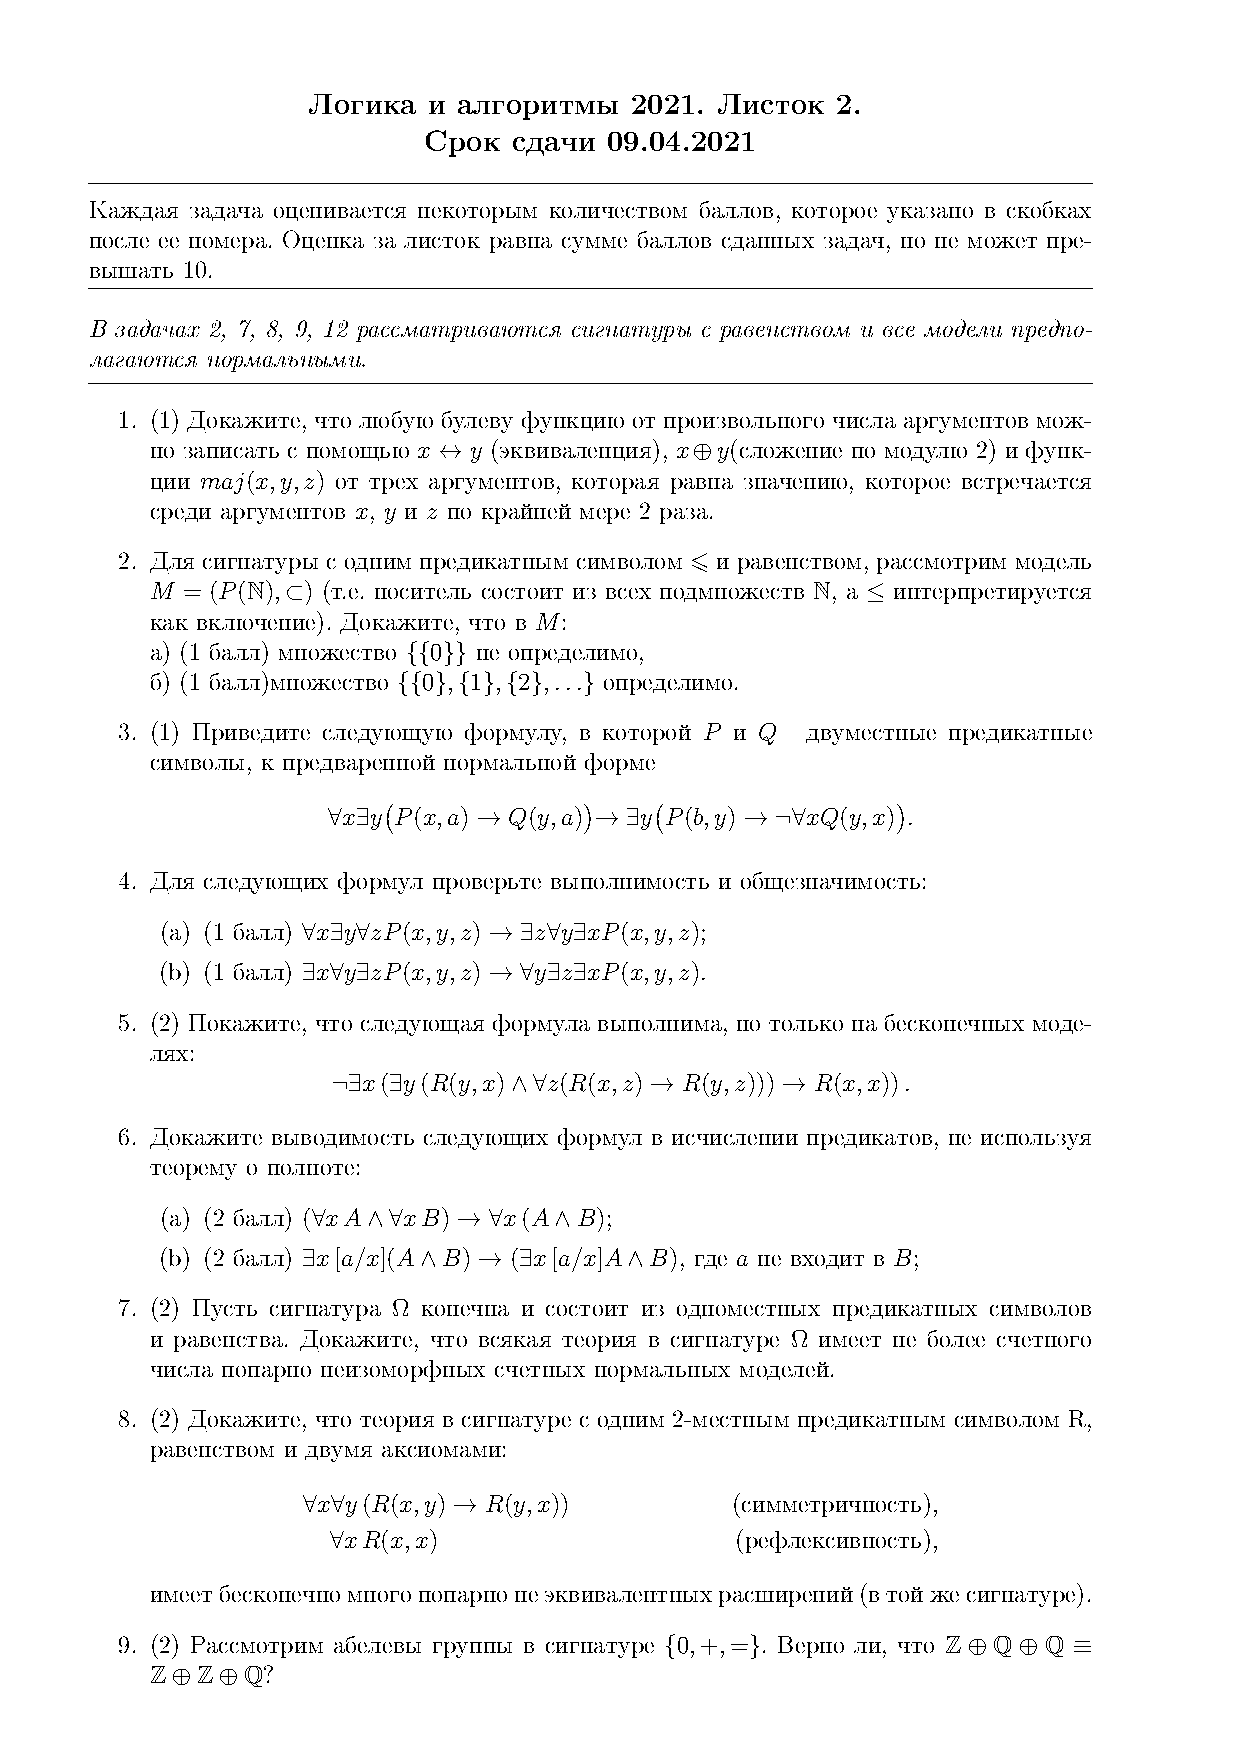
\includepdf[scale=1,pages=1-2]{Tasks/listok2}
\newpage
\section*{Решения}
\subsection*{Задача 1}
	Теорема о функциональной полноте. Для любой функции $\varphi: \mathbb{B}^n \to \mathbb{B}$ найдется такая формула $A$ от $n$ переменных, что $\varphi = \varphi_{A}$. При этом можно считать, что $A$ содержит лишь связки $\neg$ и $\vee$.\\
	Следовательно если выразить $\neg$ и $\vee$ через $x \leftrightarrow y,\ x \oplus y,\ \operatorname{maj}(x,y,z)$\\
	\begin{gather*}
	\begin{tabular}{ c c c c c c }
		x & y & x \leftrightarrow y & x \oplus y & \operatorname{maj}(x, y, x \oplus y) & x \oplus (x \leftrightarrow x)\\
		0 & 0 & 1 & 0 & 0 & 1\\
		0 & 1 & 0 & 1 & 1 & 1\\
		1 & 0 & 0 & 1 & 1 & 0\\
		1 & 1 & 1 & 0 & 1 & 0
	\end{tabular}
	\end{gather*}
	Заметим, что $\operatorname{maj}(x, y, x \oplus y)$ соответствует $x \vee y$, а $x \oplus (x \leftrightarrow x) = x \oplus 1$ соответствует $\neg x$, а следовательно любую булеву функцию можно записать, используя только данные по условию функции.

\subsection*{Задача 2}
\begin{enumerate}
\item[(a)] Рассмотрим отображение, такое что $\{0\} \leftrightarrow \{1\}$. Покажем, что это автоморфизм, то есть что если $A \subseteq B$, то $A' \subseteq B'$. Пусть $a \in A'$
	\begin{gather*}
		a \ne 0,1 \Rightarrow a \in A \Rightarrow a \in B \Rightarrow a \in B'\\
		a = 0 \Rightarrow 1 \in A \Rightarrow 1 \in B \Rightarrow 0 \in B'\\
		a = 1 \Rightarrow 0 \in A \Rightarrow 0 \in B \Rightarrow 1 \in B'
	\end{gather*}
	Итак, множество $\{\{0\}\}$ не сохранилось при рассмотренном автоморфизме, а определимые множество сохраняются при любом автоморфизме, а следовательно $\{\{0\}\}$ не явояется определимым.

\item[(b)]
	Зададим предикат, выражающий свойство одноэлементности множества, то есть всякое подмножество данного множества или пусто, или совпадает с ним самим. Выразим свойство пустоты множества ($x = \{\}$) формулой $\forall y\ x \leqslant y$, а также свойство равенства двух подмножеств ($x = y$) формулой $(x \leqslant y) \wedge (y \leqslant x)$. Через это мы можем выразить свойство одноэлементности $\forall y ((y \leqslant x) \to ((y = \{\}) \vee (y = x)))$.
\end{enumerate}
\vskip 0.4in

\subsection*{Задача 3}
	\begin{gather*}
		\forall x \exists y(P(x,a) \to Q(y,a)) \to \exists y(P(b,y) \to \neg \forall x Q(y,x))\\
		\forall x \exists y(P(x,a) \to Q(y,a)) \to \exists z(P(b,z) \to \neg \forall t Q(z,t))\\
		\forall x \exists y(\neg P(x,a) \vee Q(y,a)) \to \exists z(\neg P(b,z) \vee \neg \forall t Q(z,t))\\
		\neg \forall x \exists y(\neg P(x,a) \vee Q(y,a)) \vee \exists z(\neg P(b,z) \vee \neg \forall t Q(z,t))\\
		\neg \forall x \exists y(\neg P(x,a) \vee Q(y,a)) \vee \exists z(\neg P(b,z) \vee \exists t \neg Q(z,t))\\
		\exists x \forall y \neg (\neg P(x,a) \vee Q(y,a)) \vee \exists z(\neg P(b,z) \vee \exists t \neg Q(z,t))\\
		\exists x \forall y \exists z \exists t \neg (\neg P(x,a) \vee Q(y,a)) \vee (\neg P(b,z) \vee \neg Q(z,t))\\
		\exists x \forall y \exists z \exists t (P(x,a) \wedge \neg Q(y,a)) \vee (\neg P(b,z) \vee \neg Q(z,t))\\
		\exists x \forall y \exists z \exists t (P(x,a) \vee \neg P(b,z) \vee \neg Q(z,t)) \wedge (\neg Q(y,a) \vee \neg P(b,z) \vee \neg Q(z,t))\\
	\end{gather*}
\vskip 0.4in

\subsection*{Задача 4}
\begin{enumerate}
\item[(a)]
	\begin{gather*}
		\forall x \exists y \forall z P(x,y,z) \to \exists z \forall y \exists x P(x,y,z)
	\end{gather*}
	Рассмотрим модель целых чисел, в которой $P(x,y,z):\ y = x^2$. Тогда $\forall x \exists y \forall z (y = x^2)$ верно, а $\exists z \forall y \exists x (y = x^2)$ неверно, следовательно формула необщезначима.
\item[(b)]
	\begin{gather*}
		\exists x \forall y \exists z P(x,y,z) \to \forall y \exists z \exists x P(x,y,z)
	\end{gather*}
	Если левая часть -- истина, то существуют такие $x_0, z_0$, что $\forall y:\ P(x,y,z) \equiv 1$, тогда правая часть также истина, так как для этой же пары $x_0, z_0$ все будет выполнено, а следовательно формула истина. Если левая часть ложна, то следствие может быть любым, а следовательно формула также истина. Тогда она всегда истина, а следовательно выполнима и общезначима
\end{enumerate}
\vskip 0.4in

\subsection*{Задача 5}
	\begin{gather*}
		\neg \exists x(\exists y(R(y,x) \wedge \forall z(R(x,z) \to R(y,z))) \to R(x,x))\\
		\forall x \neg (\exists y(R(y,x) \wedge \forall z(R(x,z) \to R(y,z))) \to R(x,x))\\
		\forall x \neg (\exists y(R(y,x) \wedge \forall z(\neg R(x,z) \vee R(y,z))) \to R(x,x))\\
		\forall x \neg ( \neg \exists y(R(y,x) \wedge \forall z(\neg R(x,z) \vee R(y,z))) \vee R(x,x))\\
		\forall x (\exists y(R(y,x) \wedge \forall z(\neg R(x,z) \vee R(y,z))) \wedge \neg R(x,x))\\
		\forall x \neg R(x,x) \wedge \forall x \exists y (R(y,x) \wedge \forall z (\neg R(x,z) \vee R(y,z)))\\
		\forall x \neg R(x,x) \wedge \forall x \exists y \forall z (R(y,x) \wedge (\neg R(x,z) \vee R(y,z)))\\
		\forall x \exists y \forall z (\neg R(x,x) \wedge R(y,x) \wedge (\neg R(x,z) \vee R(y,z)))
	\end{gather*}

	\begin{comment}
		\forall x \neg R(x,x) \wedge \forall x \forall y \forall z (R(x,y) \wedge R(y,z) \to R(x,z)) \wedge \forall x\exists y R(x,y)\\
		\forall x \neg R(x,x) \wedge \forall x \forall y \forall z (\neg(R(x,y) \wedge R(y,z)) \vee R(x,z)) \wedge \forall x\exists y R(x,y)\\
		\forall x \neg R(x,x) \wedge \forall x \forall y \forall z (\neg R(x,y) \vee \neg R(y,z) \vee R(x,z)) \wedge \forall x\exists y R(x,y)
	Заметим что эта формула представляет из себя 2 аксиомы арифметики Пеано: $\forall x \exists y S(x) = y$ что то же самое что $\forall x \exists y R(x,y)$ и $\forall x \forall y S(x) = S(y) \to x = y$, что то же самое что $\forall x \forall y \forall z R(y,x) \wedge (\neg R(x,z) \vee R(y,z))$, этих аксиом достаточно для того, чтобы доказать бесконечность натуральных чисел, а следовательно данная форма выполнена только для бесконечных моделей
	\end{comment}
\vskip 0.4in

\subsection*{Задача 6}
\begin{enumerate}
\item[(a)]
	Правило Бернайса $\frac{A \to B}{A \to \forall x B[a/x]}$, следовательно нам достаточно доказать, что $(\forall x A \wedge \forall x B) \to A \wedge B$ выводимо.\\
	Применим теорему о дедукции: $\Gamma \vee \{P\} \vdash Q \Leftrightarrow \Gamma \vdash P \to Q$, то есть будем выводить $A \wedge B$ из аксиом и $(\forall x\ A \wedge \forall x\ B)$\\
	Аксиомы:\\
	$A \wedge B \to A$ (1), $A \wedge B \to B$ (2), $A \to (B \to A \wedge B)$ (3)\\
	$\forall x A[a/x] \to A[a/t]$ (4), $A[a/t] \to \exists x A[a/x]$ (5)\\
	Modus ponens: $\frac{A,\ A \to B}{B}$ (MP)
	\begin{gather*}
		\forall x A \wedge \forall x B \xrightarrow{\text{(1)}}
		\forall x A \xrightarrow{\text{(4)}}
		A \xrightarrow{\text{(*)}}
		A \wedge B
		\\
		\forall x A \wedge \forall x B \xrightarrow{\text{(2)}}
		\forall x B \xrightarrow{\text{(4)}}
		B\\
		\\
		\text{(*): } (A \to (B \to A \wedge B)) \xrightarrow{\text{(MP)}}
		(A \to A \wedge B) \xrightarrow{\text{(MP)}}
		A \wedge B
	\end{gather*}
\begin{comment}
\item[(b)]
	Правило Бернсайса: $\frac{B \to A}{\exists x\ B[a/x] \to A}$, следовательно достаточно доказать, что $A \wedge B \to \exists x [a/x]A \wedge B$ выводимо.\\
	Аналогично по теореме о дедукции выведем $\exists x [a/x] A \wedge B$ из аксиом $A \wedge B$
	\begin{gather*}
		A \wedge B\\
		A \text{ -- (1)}\\
		\exists x [a/x] A \text{ -- (5)}\\
		(B \to \exists x [a/x] A \wedge B) \text{ -- (3)}\\
		\exists x [a/x] A \text{ -- (MP)}\\
		\exists x [a/x] A \wedge B \text{ -- (MP)}
	\end{gather*}
	(в (3) в качестве $A$ выступает $\exists x [a/x] A$, в качестве $B -- B$)
	и
	\begin{gather*}
		A \wedge B\\
		B \text{ -- (2)}
	\end{gather*}
\end{comment}	
\end{enumerate}
\vskip 0.4in

\subsection*{Задача 9}
	Рассмотрим формулу
	\begin{gather*}
		\forall x (\forall s\ x \ne s + s) \to (\forall y (\forall t\ y \ne t + t) \to \exists w\ x + y = w + w)
	\end{gather*}
	Пусть $\mathbb{Z} \oplus \mathbb{Q} \oplus \mathbb{Q} = M_1,\ \mathbb{Z} \oplus \mathbb{Z} \oplus \mathbb{Q} = M_2$
	\vskip 0.1in
	Эта формула всегда верна в $M_1$:\\
	Пусть $x \ne s + s\ \forall s$, это значит, что $x = (\text{нечетное}, \text{любое}, \text{любое})$, так как га второй и третьей позиции рациональные числа, там можно любое число представить в виде $\frac{\text{число}}{2}$. Пусть $y \ne t+t$, тогда аналог $y = (\text{нечетное}, \text{любое}, \text{любое})$. Тогда $x + y = (\text{нечетное}, \text{любое}, \text{любое}) + (\text{нечетное}, \text{любое}, \text{любое}) = (\text{четное}, \text{любое}, \text{любое})$, то есть формула примет вид $1 \to (1 \to 1) = 1$\\
	Если $x \ne s + s,\ y = t + t$, то $x + y = (\text{нечетное}, \text{любое}, \text{любое})$ и формула примет вид $1 \to (0 \to 0) = 1 \to 1 = 1$\\
	Если $x = s + s,\ y \ne t + t$, то $x + y = (\text{нечетное}, \text{любое}, \text{любое})$ и формула примет вид $0 \to (1 \to 0) = 0 \to 0 = 1$\\
	Если $x = s + s,\ y = t + t$, то $x + y = (\text{четное}, \text{любое}, \text{любое})$ и формула примет вид $0 \to (0 \to 1) = 0 \to 1 = 1$
	\vskip 0.1in
	Но в $M_2$ эта формула не всегда верна, рассмотрим следующий случай:\\
	$x = (1,0,0),\ y = (0,1,0),\ x + y = (1,1,0)$. Тогда формула примет вид $1 \to (1 \to 0) = 1 \to 0 = 0$, то есть они не изоморфны и утверждение задачи неверно.
\newpage		
	\section*{Лист 3}
		\subsection*{1}
		\noindent
		Идеальный треугольник состоит из 3 вершин и 3 сторон(геодезических), а следовательно имеет ту же группу симметрий что и граф $K_3$, то есть $D_3$.
		
		\subsection*{2}
		\begin{figure}[h!]
			\begin{minipage}[h]{0.5\linewidth}
				\center{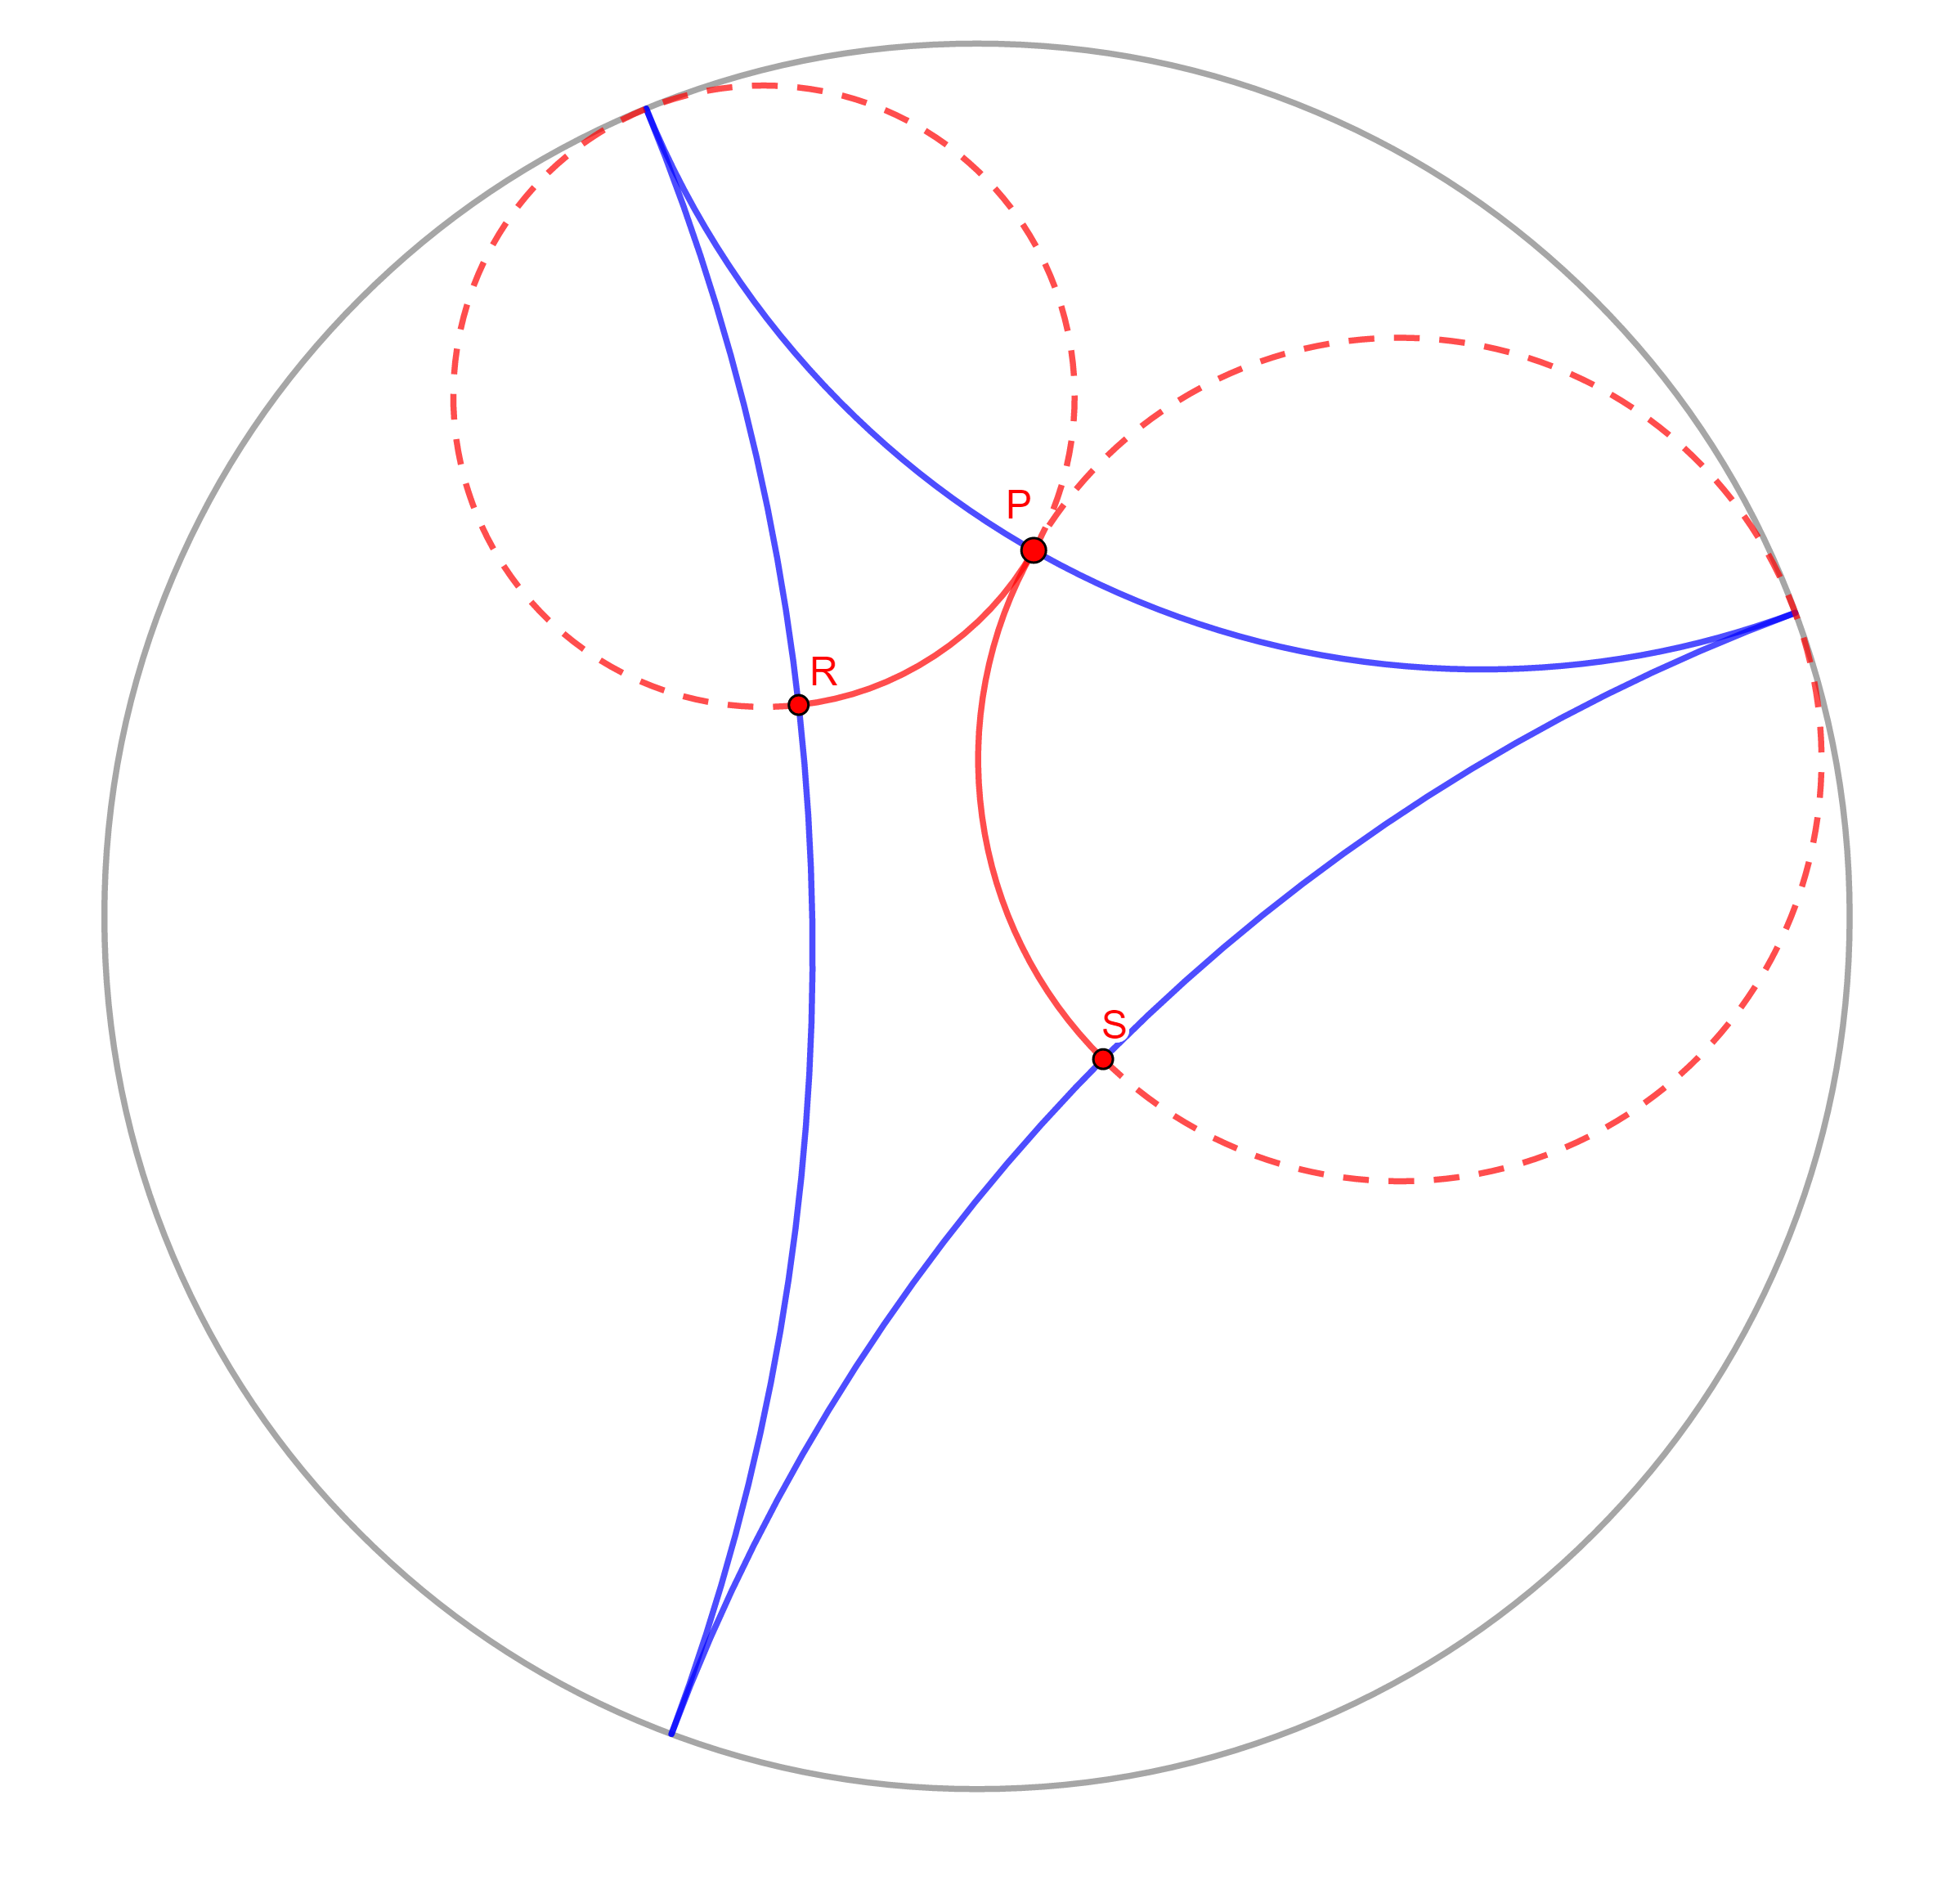
\includegraphics[width=0.7\linewidth]{pic11}}
			\end{minipage}
			\hfill
			\begin{minipage}[h]{0.5\linewidth}
				\center{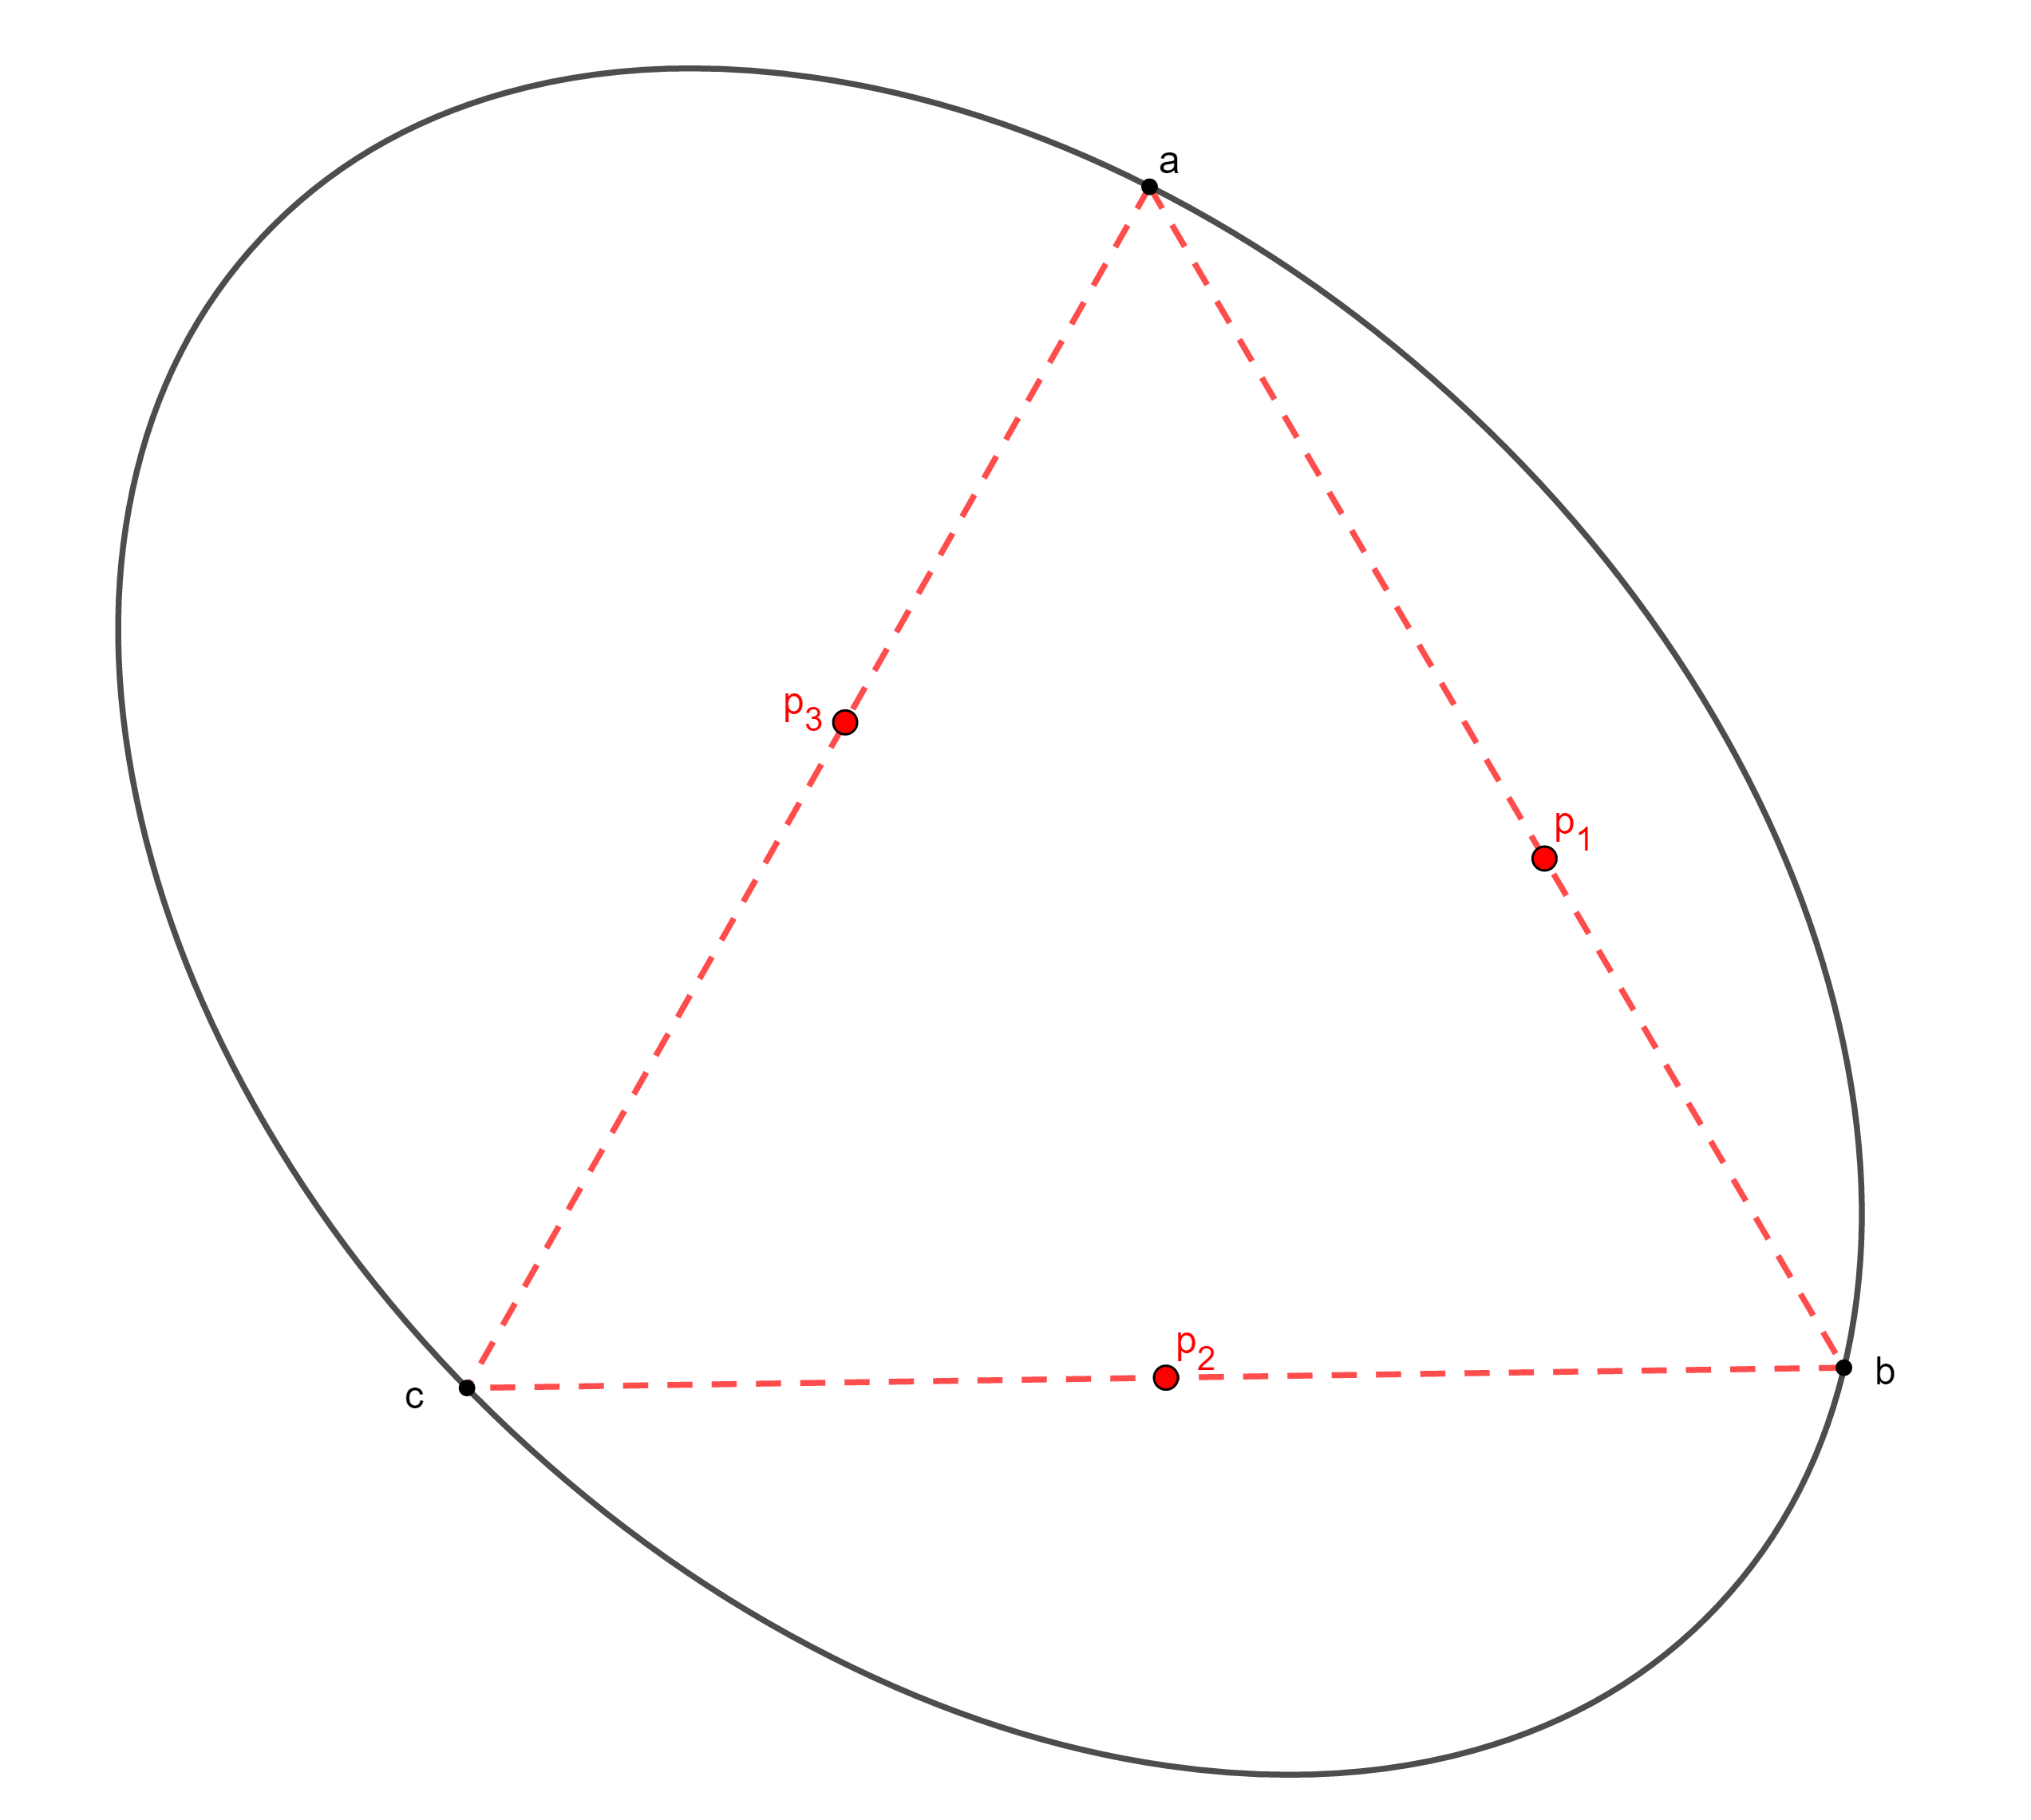
\includegraphics[width=0.8\linewidth]{pic15}}
			\end{minipage}
		\end{figure}
		\noindent
		Проведем преобразование как в одной из задач прошлого листочка -- представим наш треугольник в верхней полуплоскости с вершинами в точках $0,1,\infty$. Тогда можно заметить что $PS$ и $PR$ являются дугами орициклов. Докажем этот факт, рассмотрим картинку в верхней полуплоскости и заметим, что касательные к сторонам из точек $R,S$ совпадают с вертикальными сторонами, а следовательно центры окружностей (геодезических или орициклов), на которой лежат дуги $PS$ и $PR$, лежат на этих сторонах, а так как касательная проходящая через $P$ пересекает вертикальные стороны не в вершине, то $PS$ и $PR$ лежат на орициклах. Следовательно $\angle RPS$ это угол между орициклами, отмеченными на картинках красным. Тогда остается заметить, что эти орициклы касаются, а следовательно $\angle RPS = 0$.
		
		\subsection*{3}
		\noindent
		Заметим, что так как $\Gamma_i = e^{\frac{1}{2}a_i}$ то установив биекцию между треугольниками и тройками $(a_i,a_j,a_k)$ мы также установим биекцию между треугольниками и $(\Gamma_i, \Gamma_j,\Gamma_k)$, так как $\Gamma_i = e^{\frac{1}{2}a_i}$ задает биекцию между $(a_i,a_j,a_k)$ и $(\Gamma_i, \Gamma_j,\Gamma_k)$.
		\begin{figure}[h!]
			\center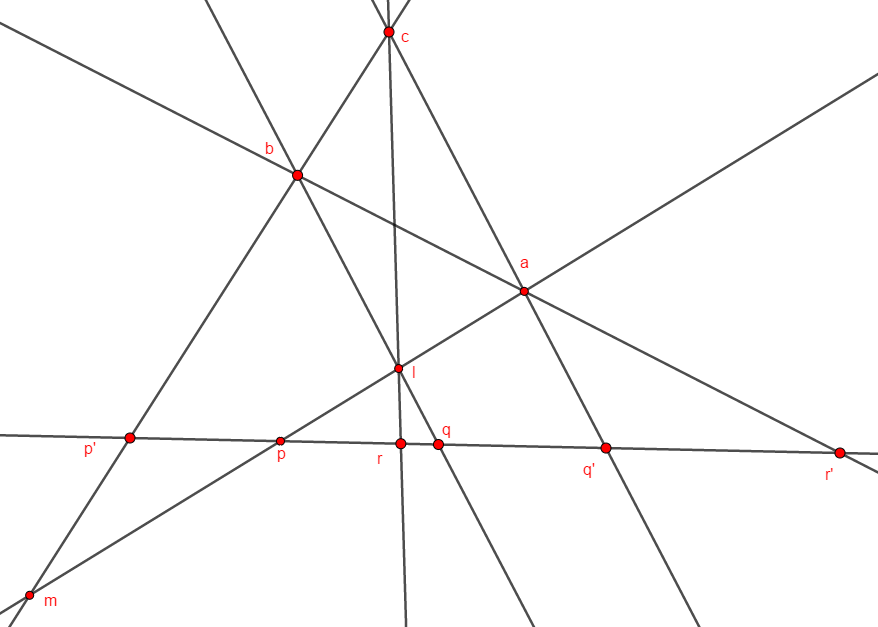
\includegraphics[width=0.5\linewidth]{pic9}
		\end{figure}\\
		Рассмотрим картинку, где красным отмечены орициклы $O_1, O_2, O_3$. Тогда заметим что участки геодезических отмеченные одним цветом(зеленым, оранжевым или фиолетовым) имеют равную длину и их длины мы можем вывести из $a_1, a_2, a_3$ (так как мы можем составить систему из 3 уравнений с 3 неизвестными). Также заметим, что по задаче 4 мы знаем $c_1, c_2, c_3$. Остается заметить, что из этого мы можем вывести длину цветных (зеленых, фиолетовых или рыжих) при любом размере красных орициклов, а следовательно и в случае нулевого радиуса, тогда мы получим длину 3 сторон, по которым однозначно восстанавливается идеальный треугольник.\\
		
		\subsection*{4}
		\begin{gather*}
			c_k = \frac{\Lambda_k}{\Lambda_i \Lambda_j} = \frac{e^{\frac{1}{2}a_{k}}}{e^{\frac{1}{2}a_{i}} e^{\frac{1}{2}a_{j}}} = e^{\frac{1}{2}a_{k}} \cdot e^{-\frac{1}{2}a_{i}} \cdot e^{-\frac{1}{2}a_{j}} = e^{\frac{1}{2}(a_{k} - a_{i} - a_{j})}
		\end{gather*}
		
		\subsection*{5*}
		\noindent
		Рассмотрим синий орицикл
		\begin{figure}[h]
			\center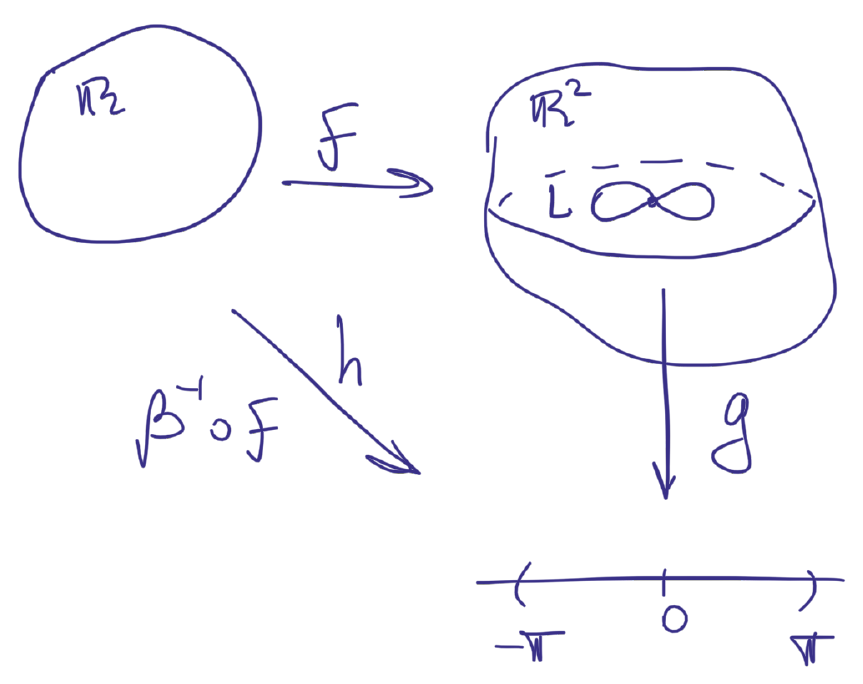
\includegraphics[width=0.65\linewidth]{pic10}
		\end{figure}\\
		Заметим что для дуги отмеченной красным выполнено:
		\begin{gather*}
			c_{13} = c_{12} + c_{23}\\
			\\
			\frac{\Lambda_{13}}{\Lambda_{14}\Lambda_{34}} = \frac{\Lambda_{12}}{\Lambda_{14}\Lambda_{24}} + \frac{\Lambda_{23}}{\Lambda_{24}\Lambda_{34}}
		\end{gather*}
		Домножим на $\Lambda_{14}\Lambda_{24}\Lambda_{34}$
		\begin{gather*}
			\Lambda_{13}\Lambda_{24} = \Lambda_{12}\Lambda_{34} + \Lambda_{23}\Lambda_{14}
		\end{gather*}
		
		\begin{comment}
		\subsection*{6*}
		\noindent
		Заметим что для всех треугольников данной фигуры должно быть выполнено неравенство треугольника 
		\begin{gather*}
		\end{gather*}
		\end{comment}
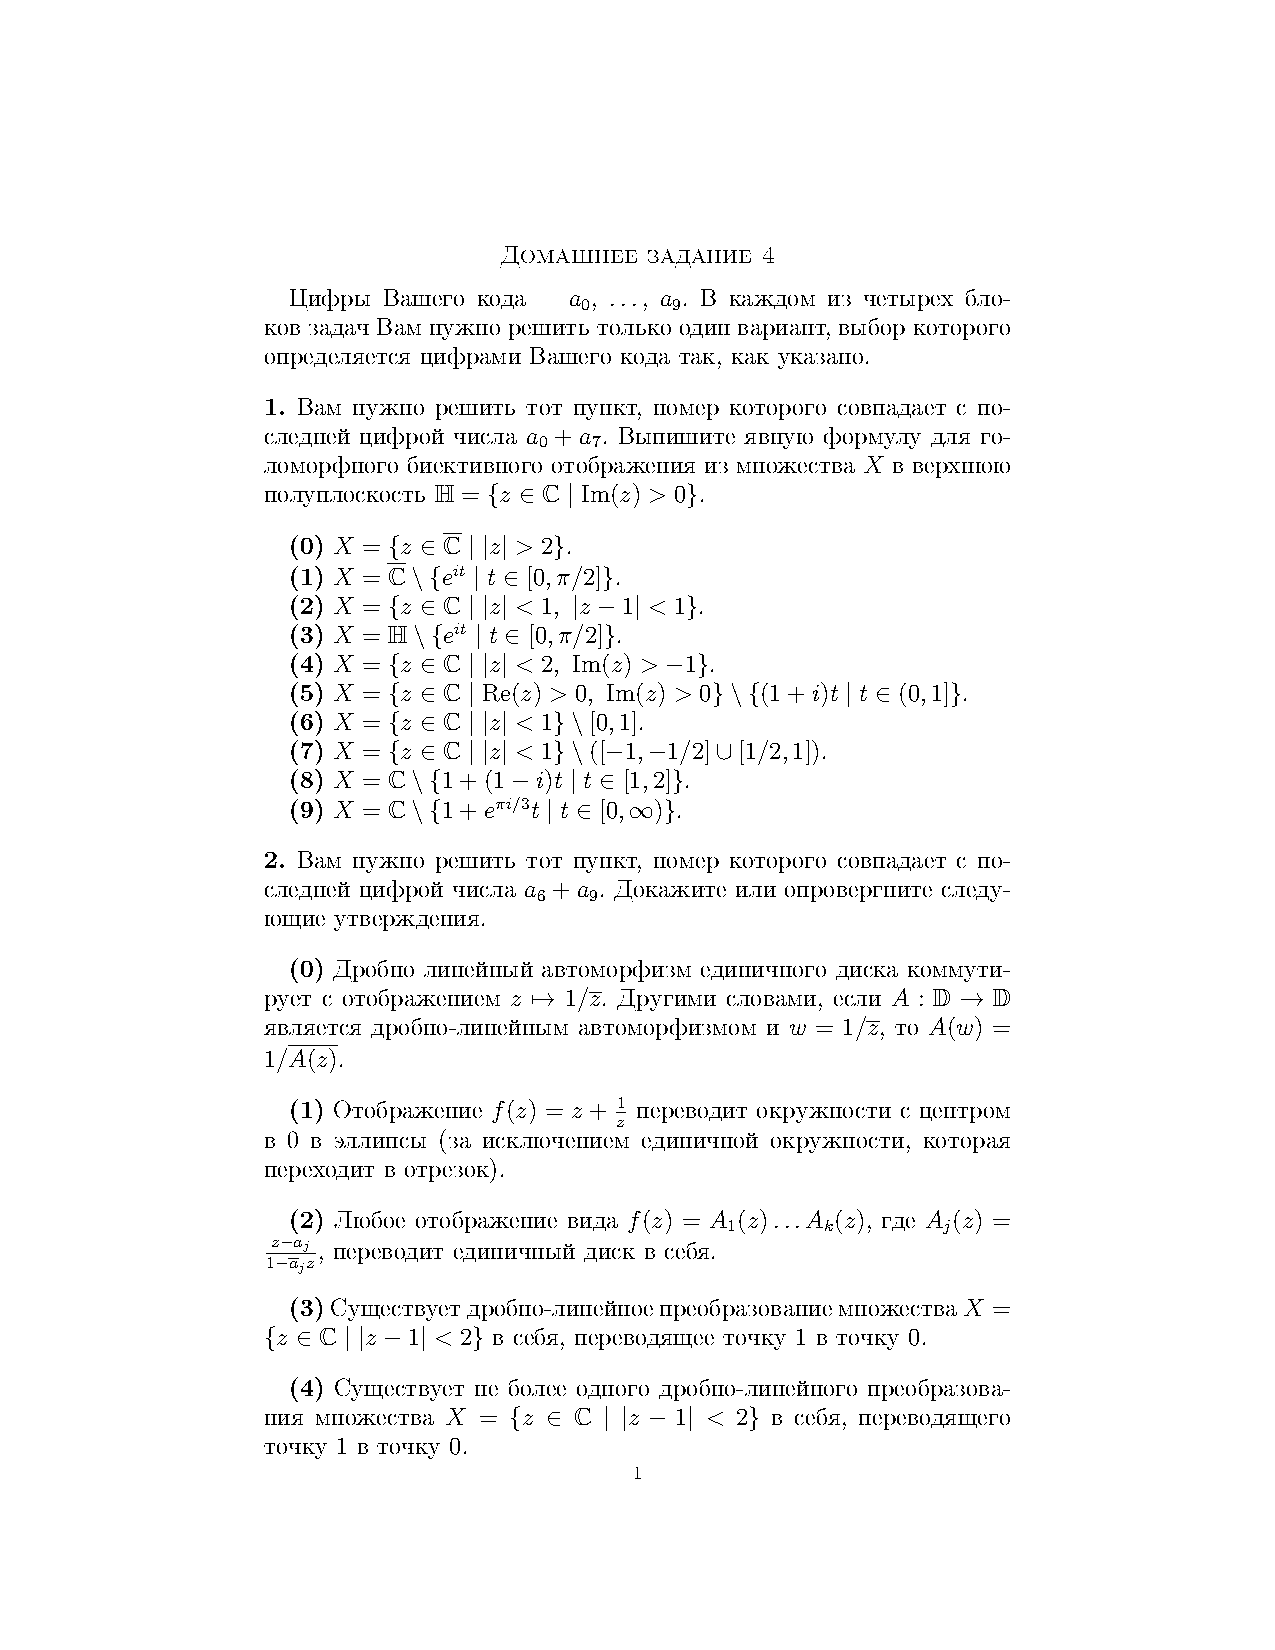
\includepdf[scale=1,pages=1-4]{Tasks/hw4}
\newpage
\section*{Решения}
\subsection*{Задача 1}
	Необходимо решить задачу $a_0 + a_7 = 1 + 3 = 4 \mod 10$
	\begin{gather*}
		X = \{z \in \mathbb{C}|\ |z| < 2,\ \Im(z) > -1\}\qquad
		\mathbb{H} = \{z \in \mathbb{C}|\ \Im(z) > 0\}
	\end{gather*}
	Заметим, что у $X$ есть 2 угла $\frac{2\pi}{3}$, тогда переведем один из них (пусть это будет точка $\sqrt{3}-i$) на бесконечность, а второй ($-\sqrt{3}-i$) в 0. И тогда, чтобы угол $\frac{2\pi}{3}$ стал равным $\pi$, необходимо возвести итоговое отображение в степень $\frac{3}{2}$.
	\begin{gather*}
		f(z) = \frac{az + b}{cz + d}\\
		\begin{cases}
			f(\sqrt{3}-i) = \frac{a(\sqrt{3}-i) + b}{c(\sqrt{3}-i) + d} = \infty\qquad
			c(\sqrt{3}-i) + d = 0\\
			f(-\sqrt{3}-i) = \frac{a(-\sqrt{3}-i) + b}{c(-\sqrt{3}-i) + d} = 0\qquad
			a(-\sqrt{3}-i) + b = 0
		\end{cases}\\
		f(z) = \frac{az + (\sqrt{3}+i)a}{cz + (i - \sqrt{3})c}
		= \frac{a}{c}\cdot\frac{z + i + \sqrt{3}}{z + i - \sqrt{3}}\\
		f_1(z) = f(z)^{\frac{3}{2}}
		= \left(\frac{a}{c}\cdot\frac{z + i + \sqrt{3}}{z + i - \sqrt{3}}\right)^{\frac{3}{2}}
	\end{gather*}
	Осталось заметить, что данное преобразование дает нам полуплоскость $\{\Re(z) < 0\}$, это можно проверить, посмотрев куда переходит центр окружности $\frac{0 + i + \sqrt{3}}{0 + i - \sqrt{3}}^{\frac{3}{2}} = -1$, тогда для получения отображения необходимо повернуть все на $\frac{\pi}{2}$ против часовой стрелки, то есть домножить на $-i$, откуда
	\begin{gather*}
		F(z) = -i \cdot \left(\frac{a}{c}\cdot\frac{z + i + \sqrt{3}}{z + i - \sqrt{3}}\right)^{\frac{3}{2}},\quad \frac{a}{c} \in \mathbb{R}
	\end{gather*}
\vskip 0.4in

\subsection*{Задача 2}
	Необходимо решить задачу $a_6 + a_9 = 9 + 6 = 5 \mod 10$\\
	Мы можем задать окружность 3 точками, поэтому будем рассматривать автоморфизм $(x_1, x_2, x_3) \mapsto (y_1, y_2, y_3)$, обозначим его как $\Phi$ и $\Phi(x_i) = y_i$. Заметим, что $\operatorname{PSL}(2, \mathbb{R})$ -- автоморфизмы верхней полуплоскости и
	\begin{gather*}
		z \to \frac{az + b}{cz + d}\\
		ad - bc = 1\\
		(a,b,c,d) \sim (\alpha a, \alpha b,\alpha c,\alpha d)
	\end{gather*}
	То есть эти матрицы задаются 3 параметрами (так как 4 получается из $ad - bc = 1$). Тогда заметим, что у нас есть система из 4 уравнений с 4 неизвестными:
	\begin{gather*}
		\frac{ax_1 + b}{cx_1 + d} = y_1\qquad
		\frac{ax_2 + b}{cx_2 + d} = y_2\qquad
		\frac{ax_3 + b}{cx_3 + d} = y_3\qquad
		ad-bc = 1
	\end{gather*}
	У это системы есть хотя бы одно решение, а следовательно есть и автоморфизм, переводящий одну окружность в другую.
	\begin{comment}
	Заметим, что можно построить биекцию из любого круга в любую полуплоскость, для определенности, $\mathbb{H} = \{\Im(z) > 0\}$, тогда если есть 2 круга $O_1, O_2$, то можно построить две биекции $f_1: O_1 \to \mathbb{H},\ f_2: \mathbb{H} \to O_2$ и $f_1 \circ f_2$ будет биекцией $O_1 \to O_2$, при это граница биективно отобразилась в границу, что и требовалось. 
	\end{comment}
\vskip 0.4in

\subsection*{Задача 3}
	Необходимо решить задачу $a_3 + a_9 = 9 + 6 = 5 \mod 10$
	\begin{gather*}
		U = \{x > y > 0\},\ (a,b) = (2, 1)
	\end{gather*}
	Переведем нашу область в полуплоскость, получим отображение
	$f_1(z) = z^4$ и $(2,1)$ перейдет в $(-7, 24)$.\\
	Теперь переведем полуплоскость $\mathbb{H}$ в окружность, но сперва переведем $(-7,24)$ в $(0,1)$
	\begin{gather*}
		f_2(z) = \frac{z+7}{24}\\
		f_3(z) = \frac{z-i}{z+i}\\
		f(z) = f_1 \circ f_2 \circ f_3
		= \frac{\frac{z^4+7}{24} - i}{\frac{z^4+7}{24} + i}
		= \frac{z^4 + 7 - 24i}{z^4 + 7 - 24i} 
	\end{gather*}
	Возьмем логарифм от $f(z)$, он перведет центр окружности в бексонечность, а края в 0, что и трбовалось
	\begin{gather*}
		F(z) = \log(f(z))
		= \log\left( \frac{z^4 + 7 - 24i}{z^4 + 7 - 24i} \right)
	\end{gather*}

\vskip 0.4in
\subsection*{Задача 4}
	Необходимо решить задачу $3a_7 = 3 \cdot 3 = 9 \mod 10$
	\begin{gather*}
		X = \{z = x + iy|\ 0<x<\frac{\pi}{2}\},\quad f(z) = \sin(z)\\
		\sin(z)
		= \sin(x + iy)
		= \sin(x)\cos(iy) + i\cos(x)\sin(iy)
		= \sin(x)\cosh(y) + i\cos(x)\sinh(y)\\
		\Re(\sin(z)) = \sin(x)\cosh(y),\quad \Im(\sin(z)) = \cos(x)\sinh(y)
	\end{gather*}
	Заметим что есть период $2\pi$, а следовательно достаточно рассмотреть $x \in (-\pi, \pi)$. Заметим, что
	\begin{gather*}
		u \left(\frac{\pi}{2} - x, y \right) = u\left( \frac{\pi}{2}+x, -y \right)\\
		v \left(\frac{\pi}{2}-x, y \right) = v \left( \frac{\pi}{2}+x, -y\right)
	\end{gather*}
	Тогда
	\begin{figure}[h]
	\begin{minipage}[h]{0.5\linewidth}
		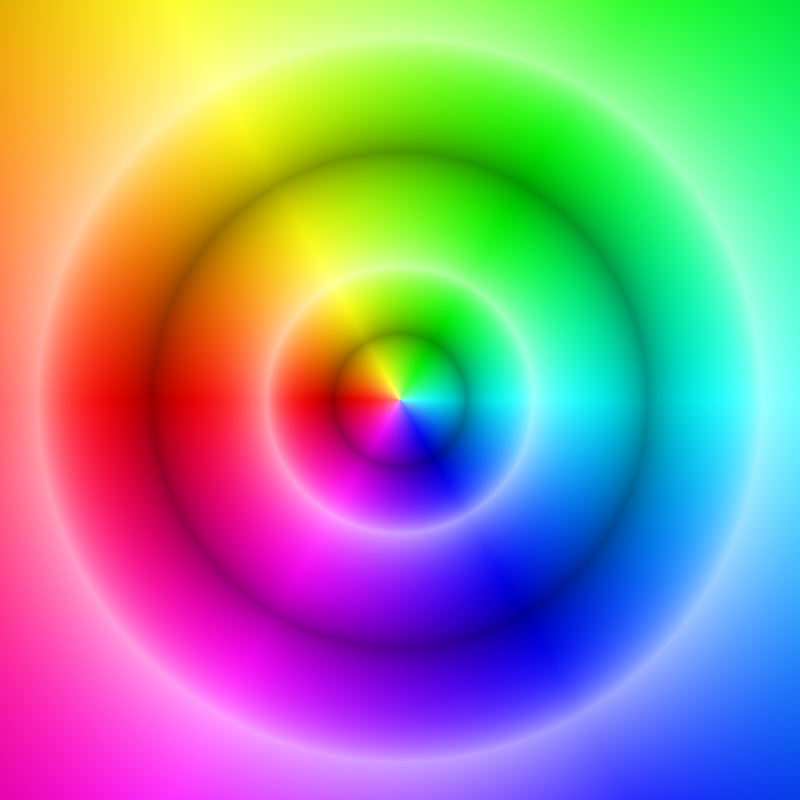
\includegraphics[width=0.95\linewidth]{Pic3}
		\caption{Комплексная плоскость}
	\end{minipage}
	\hfill
	\begin{minipage}[h]{0.5\linewidth}
		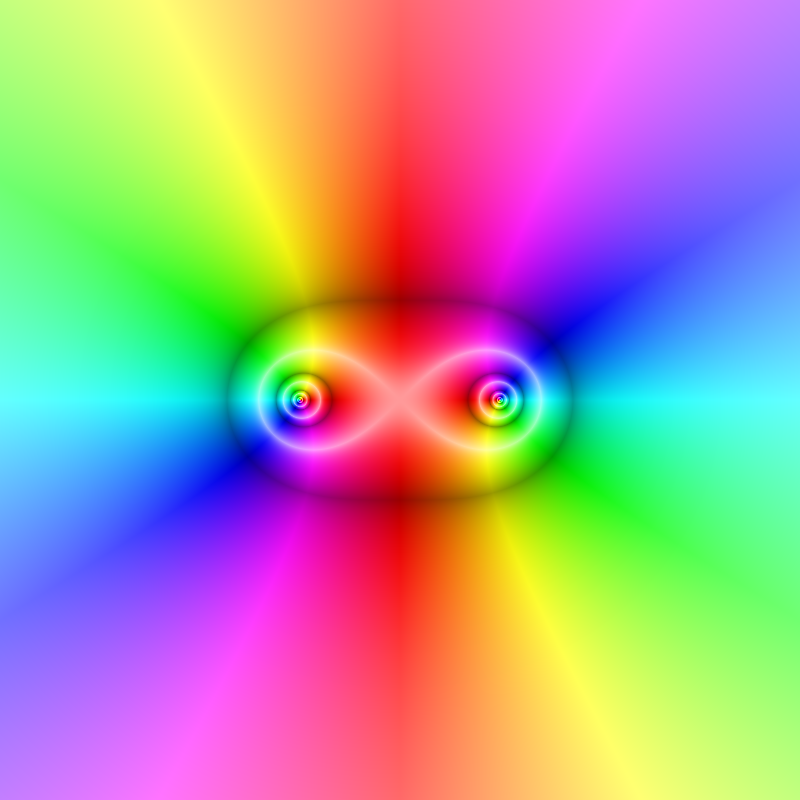
\includegraphics[width=0.95\linewidth]{Pic4}
		\caption{Плоскость после преобразования $\sin z$ на $X$}
	\end{minipage}
	\end{figure}
\vskip 0.4in

\begin{comment}
\subsection*{Задача 5}
	Необходимо решить задачу $a_1 + a_8 = 7 + 8 = 5 \mod 10$
\end{comment}
\newpage
	{\large \hspace{3cm} \begin{center} Домашнее задание 18 $\bullet$ Мозговой Владислав \end{center} }
	\vspace{-1.5ex}
	\hrulefill
	
	\fontsize{12pt}{4.5mm}\selectfont
	\vspace{-3ex}
	\hrulefill
	\newline

	\section{}
		\subsection*{\textbf{Задача 1}}
		Пусть $G$ -- факторгруппа свободной абелевой группы $\mathbb{Z}^{4}$ по подгруппе порождённой строками матрицы
		\begin{gather*}
			\begin{bmatrix}
				{-130} & {245} & {0} & {120} \\
				{-10} & {5} & {0} & {0} \\
				{60} & {-80} & {20} & {-60} \\
				{-60} & {120} & {0} & {60}
			\end{bmatrix}
		\end{gather*}
		\subsubsection*{\textbf{А}}
		\textbf{Условие}\\
		Разложите G в прямую сумму циклических\\
		\\
		\textbf{Решение}\\
		$A = \langle a_1, a_2, a_3, a_4 \rangle$
		\begin{gather*}
			\begin{bmatrix}
				{-130} & {245} & {0} & {120} \\
				{-10} & {5} & {0} & {0} \\
				{60} & {-80} & {20} & {-60} \\
				{-60} & {120} & {0} & {60}
			\end{bmatrix}
			=
			\begin{bmatrix}
				{-130} & {245} & {0} & {120} \\
				{-10} & {5} & {0} & {0} \\
				{0} & {0} & {20} & {0} \\
				{-60} & {120} & {0} & {60}
			\end{bmatrix}
			=
			\begin{bmatrix}
				{-10} & {5} & {0} & {120} \\
				{-10} & {5} & {0} & {0} \\
				{0} & {0} & {20} & {0} \\
				{0} & {0} & {0} & {60}
			\end{bmatrix}
			=\\
			\begin{bmatrix}
				{-5} & {5} & {0} & {0} \\
				{-5} & {5} & {0} & {0} \\
				{0} & {0} & {20} & {0} \\
				{0} & {0} & {0} & {60}
			\end{bmatrix}
			=
			\begin{bmatrix}
				{-5} & {0} & {0} & {0} \\
				{-5} & {0} & {0} & {0} \\
				{0} & {0} & {20} & {0} \\
				{0} & {0} & {0} & {60}
			\end{bmatrix}
			=
			\begin{bmatrix}
				{5} & {0} & {0} & {0} \\
				{0} & {0} & {20} & {0} \\
				{0} & {0} & {0} & {60}
			\end{bmatrix}
		\end{gather*}
		$A \simeq \mathbb{Z}_5 \oplus \mathbb{Z}_20 \oplus \mathbb{Z}_60 \oplus \mathbb{Z}$\\
		
		\subsubsection*{\textbf{Б}}
		\textbf{Условие}\\
		Разложите G в прямую сумму примарных циклически\\
		\\
		\textbf{Решение}\\
		$A \simeq \mathbb{Z}_{2^4} \oplus \mathbb{Z}_{3} \oplus \mathbb{Z}_{5^3}$\\
		
		\subsubsection*{\textbf{В}}
		\textbf{Условие}\\
		Чему равен максимальный возможный порядок её элементов\\
		\\
		\textbf{Решение}\\
		Рассмотрим элементы вида $[\alpha, \beta, \gamma, 0]$\\
		Пусть $A^{\prime} = \mathbb{Z}_5 \oplus \mathbb{Z}_20 \oplus \mathbb{Z}_60$\\
		Тогда порядок элемента $[\alpha, \beta, \gamma, 0]$ в $A$ равен порядку элемента $[\alpha, \beta, \gamma]$ в $A^{\prime}$\\
		$[\alpha, \beta, \gamma]$ -- НОК порядков $\alpha$ в $\mathbb{Z}_{5}$, $\beta$ в $\mathbb{Z}_{20}$, $\gamma$ в $\mathbb{Z}_{60}$, откуда максимальный порядок элемента это 60, такой порядок достигается у $[1,1,1]$\\
		
		\subsubsection*{\textbf{Г}}
		\textbf{Условие}\\
		Вычислите порядок элемента $\begin{bmatrix} {-132} & {248} & {1} & {120} \end{bmatrix}$ в группе $G$\\
		\\
		\textbf{Решение}\\
		\begin{gather*}
			\begin{bmatrix}
				{-5} & {0} & {0} & {0} \\
				{0} & {0} & {20} & {0} \\
				{0} & {0} & {0} & {60} \\
				{-132} & {248} & {1} & {120}
			\end{bmatrix}
			=
			\begin{bmatrix}
				{-5} & {5} & {0} & {0} \\
				{0} & {0} & {20} & {0} \\
				{0} & {0} & {0} & {60} \\
				{2} & {248} & {1} & {0}
			\end{bmatrix}
		\end{gather*}
		Порядок $\begin{bmatrix} {-132} & {248} & {1} & {120} \end{bmatrix}$: $\#(2)$ в $\mathbb{Z}_5$, $\#(1)$ в $\mathbb{Z}_{20}$, $\#(0)$ в $\mathbb{Z}_{60}$, откуда: 
		
		
		\subsection*{\textbf{Задача 3}}
		\textbf{Теория}\\
		Напомним, что цепным комплексом абелевых групп называется набор абелевых групп $C_n$ и отображений $d_n:\ C_n \to C_{n-1}$, таких что композиция $d_n \circ d_{n+1} = 0$ для любого $n$. Для удобства комплекс обозначают $(C\bullet , d\bullet)$ или записывают в виде цепочки отображений:
		\begin{gather*}
			\ldots \rightarrow C_{n+1} \stackrel{d_{n}+1}{\rightarrow} C_{n} \stackrel{d_{n}}{\rightarrow} C_{n-1} \stackrel{d_{n-1}}{\rightarrow} \ldots
		\end{gather*}
		$n$-мерной группой гомологий $H_n$ называется фактор-группа $\text{ker}(d_n)/\text{Im}(d_{n+1})$. Гомологиями комплекса $(C\bullet , d\bullet)$ называется набор всех групп гомологий $(H\bullet )$.
		\\
		\textbf{Условие}\\
		Вычислите гомологии комплекса
		\begin{gather*}
			0 \rightarrow \mathbb{Z}^{3} \stackrel{d}{\rightarrow} \mathbb{Z}^{4} \rightarrow 0
		\end{gather*}
		где отображение $d$ задано матрицей
		\begin{gather*}
			\begin{bmatrix}
				{14} & {-14} & {0} \\
				{14} & {126} & {140} \\
				{28} & {-308} & {-266} \\
				{0} & {-140} & {-98}
			\end{bmatrix}
		\end{gather*}
		\\
		\textbf{Решение}\\
		\begin{gather*}
			d = 
			\begin{bmatrix}
				{14} & {-14} & {0} \\
				{14} & {126} & {140} \\
				{28} & {-308} & {-266} \\
				{0} & {-140} & {-98}
			\end{bmatrix}
			\to
			\begin{bmatrix}
				{14} & {-14} & {14} \\
				{14} & {126} & {14} \\
				{28} & {-308} & {42} \\
				{0} & {-140} & {42}
			\end{bmatrix}
			\to
			\begin{bmatrix}
				{14} & {-14} & {14} \\
				{0} & {140} & {0} \\
				{0} & {-336} & {14} \\
				{0} & {-140} & {42}
			\end{bmatrix}
			\to
			\begin{bmatrix}
				{14} & {0} & {0} \\
				{0} & {140} & {0} \\
				{0} & {-336} & {14} \\
				{0} & {-140} & {42}
			\end{bmatrix}
			\to\\
			\begin{bmatrix}
				{14} & {0} & {0} \\
				{0} & {140} & {0} \\
				{0} & {-56} & {14} \\
				{0} & {0} & {42}
			\end{bmatrix}
			\to
			\begin{bmatrix}
				{14} & {0} & {0} \\
				{0} & {140} & {0} \\
				{0} & {-56} & {14} \\
				{0} & {-168} & {0}
			\end{bmatrix}
			\to
			\begin{bmatrix}
				{14} & {0} & {0} \\
				{0} & {140} & {0} \\
				{0} & {-56} & {14} \\
				{0} & {-28} & {0}
			\end{bmatrix}
			\to
			\begin{bmatrix}
				{14} & {0} & {0} \\
				{0} & {28} & {0} \\
				{0} & {0} & {14}
			\end{bmatrix}\\
			\\
			\text{ker}\: d \cong 14\mathbb{Z} \oplus 28\mathbb{Z} \oplus 14\mathbb{Z}\\
			\text{im}\: d \cong \mathbb{Z}^3\slash_{\text{ker}\: d} = 14\mathbb{Z} \oplus 14\mathbb{Z} \oplus 28\mathbb{Z}\\
			\text{ker}\: d_0 = \mathbb{Z}^4,\quad \text{im}\: d_1 = \mathbb{Z}^3
		\end{gather*}
		Ответ:
		\begin{gather*}
			H_0 = \text{ker}\: d_0 \slash \text{im}\: d = \mathbb{Z}^4 \slash \Big( \mathbb{Z}_{14} \oplus \mathbb{Z}_{14} \oplus \mathbb{Z}_{28} \Big)\\
			H_1 = \text{ker}\: d \slash \text{im}\: d_1 = \Big(14\mathbb{Z} \oplus 14\mathbb{Z} \oplus 28\mathbb{Z}\Big)\slash \mathbb{Z}^3
		\end{gather*}
\newpage
	{\large \hspace{3cm} \begin{center} Домашнее задание 19 $\bullet$ Мозговой Владислав \end{center} }
	\vspace{-1.5ex}
	\hrulefill
	
	\fontsize{12pt}{4.5mm}\selectfont
	\vspace{-3ex}
	\hrulefill
	\newline

	\section{}
		\subsection*{\textbf{Задача 1}}
		\textbf{Условие}\\
		Найдите наибольший общий делитель следующих многочленов с
		коэффициентами в поле $\mathbb{F}^2$: $f(x) = x^6+x^5+x^4+x$ и $g(x) = x^7+x^6+x^2+x+1$\\
		\textbf{Решение}\\
		По алгоритму евклида:
		\begin{gather*}
			\text{gcd}(x^7+x^6+x^2+x+1, x^6+x^5+x^4+x) = 
			\text{gcd}(x^6+x^5+x^4+x, x^5 + x + 1) = \\
			\text{gcd}(x^5 + x + 1, x^4 + x^2 + x + 1) = 
			\text{gcd}(x^4 + x^2 + x + 1, x^3 + x^2 + 1) = x^3 + x^2 + 1\\
			g(x) = (x^3 + x^2 + 1)(x^4 + x + 1)\\
			f(x) = (x^3 + x^2 + 1)(x^3 + x)
		\end{gather*}
		\\
		
		\subsection*{\textbf{Задача 2}}
		\textbf{Условие}\\
		Разложите пространство $V := \mathbb{F}_2[x]\slash(f(x))$ в прямую сумму двух $3-x$ мерных подпространств, инвариантных относительно умножения на $x$\\
		\textbf{Решение}\\
		\begin{gather*}
			V = \mathbb{F}_2[x]\slash_{f(x)} = \mathbb{F}_2[x]\slash_{x^3 + x} \oplus \mathbb{F}_2[x]\slash_{x^3 + x^2 + 1}
		\end{gather*}
		Элементы $\mathbb{F}_2[x]\slash_{x^3+x^2+1}:\ 0, 1, x, x+1, x^2, x^2+1, x^2+x, x^2+x+1$\\
		$\phi(\alpha) = x\alpha$\\
		$x(x^2+1) \equiv x^2 + x + 1\ \text{mod}(x^3+x^2+1)$\\
		$x(x^2+x+1) \equiv x + 1\ \text{mod}(x^3+x^2+1)$\\
		аналогично элементы $\mathbb{F}_2[x]\slash_{x^3+x}:\ 0, 1,\ldots$\\
		$\phi(\beta) = x\beta$\\
		Пространство инвариантно\\
		\\
		
		\subsection*{\textbf{Задача 3}}
		\textbf{Условие}\\
		Вычислите матрицу и характеристический многочлен в каждом из этих 3-мерных подпространств, выбрав подходящий базис в $V$, такой что первые 3 базисных вектора порождают первое подпространство, а последние 3 -- второе. Укажите этот базис явно\\
		\textbf{Решение}\\
		Базис в $\mathbb{F}_2[x]\slash_{x^3+x^2+1}:$
		\begin{gather*}
			a_1 = x^3 + x^2 + 1\\
			a_2 = x(x^3 + x^2 + 1)\\
			a_3 = x^2(x^3 + x^2 + 1)
		\end{gather*}
		Так как $x(e_1) = x^6 + x^5 + x^3 = x^5 + x^4 + x^2 = e_3$\\
		Базис в $\mathbb{F}_2[x]\slash_{x^3+x}:$
		\begin{gather*}
		a_1 = x^3 + x\\
		a_2 = x(x^3 + x)\\
		a_3 = x^2(x^3 + x)
		\end{gather*}
		Так как $x(e_1) = x^6 + x^4 = x^5 + x^3 = e_3$\\
		\\
		Тогда получается матрица
		\begin{gather*}
			\begin{bmatrix}
				0 & 0 & 1 & 0 & 0 & 0\\
				1 & 0 & 0 & 0 & 0 & 0\\
				0 & 1 & 0 & 0 & 0 & 0\\
				0 & 0 & 0 & 0 & 0 & 1\\
				0 & 0 & 0 & 1 & 0 & 0\\
				0 & 0 & 0 & 0 & 1 & 1
			\end{bmatrix}
		\end{gather*}
		Многочлены для $\mathbb{F}_2[x]\slash_{x^3+x}:$
		\begin{gather*}
			\begin{bmatrix}
				-\lambda & 0 & 1\\
				1 & -\lambda & 0\\
				0 & 1 & -\lambda
			\end{bmatrix}
			= -\lambda^3 + 1
		\end{gather*}
		Многочлены для $\mathbb{F}_2[x]\slash_{x^3+x^2+1}:$
		\begin{gather*}
			\begin{bmatrix}
				-\lambda & 0 & 1\\
				1 & -\lambda & 0\\
				0 & 1 & 1-\lambda
			\end{bmatrix}
			= \lambda^2(1-\lambda) + 1 = -\lambda^3 + \lambda^2 + 1
		\end{gather*}
		
		
		\subsection*{\textbf{Задача 4}}
		\textbf{Условие}\\
		Вычислите количество подпространств в $\mathbb{F}_2[x]\slash(g(x))$ инвариантных относительно умножения на $x$. Нульмерное подпространство и всё пространство также считаются подпространствами\\
		\textbf{Решение}\\
		$|\mathbb{F}_2\slash_{g(x)}| = \det(A) \cdot \det(B) = (-\lambda^3 + \lambda^2 + 1)$\\
		$\lambda = $, других вещественных корней нет $\Rightarrow$ существет  инвариантное пространство\\
		\\
		
		\subsection*{\textbf{Задача 5}}
		\textbf{Условие}\\
		Тот же вопрос о количестве $x$-инвариантных подпространств в пространстве $\mathbb{F}_2[x]/(f(x))$\\
		\textbf{Решение}\\
		Количество инвариантных подпространств равно количеству собственных значений матрицы оператора\\
		$|\mathbb{F}_2\slash_{f(x)}| = \det(A) \cdot \det(B) = (-\lambda^3 + 1)(-\lambda^3 + \lambda^2 + 1)$\\
		$\lambda = 1$, других вещественных корней нет $\Rightarrow$ существет $1+2 = 3$ инвариантных пространства\\
		\\
		
		\subsection*{\textbf{Задача 6}}
		\textbf{Условие}\\
		Тот же вопрос о количестве $x$-инвариантных подпространств в пространстве $\mathbb{F}_2[x]/(f(x)) \oplus \mathbb{F}_2[x]/(g(x))$\\
		\textbf{Решение}\\
		$|\mathbb{F}_2\slash_{f(x)}| \cdot |\mathbb{F}_2\slash_{g(x)}| = $\\
		$\lambda = $, других вещественных корней нет $\Rightarrow$ существет  инвариантное пространство\\
		\\
\section{HW 7}

\begin{prob}
Пусть $X$ схема, $f \in \mathcal{O}_X(X), X_f$ подмножество точек $X$, где $f$ не обращается в нуль (т е образ $f$ не лежит в максимальном идеале соответствующего локального кольца). Предположим, что $X$ нетерова, или же отделима и квазикомпактна. Покажите, что $X_f$ открыто и гомоморфизм ограничения индуцирует изоморфизм $\mathcal{O}_X(X)_f$ и $\mathcal{O}_X\left(X_f\right)$.
\end{prob}
\begin{proof}
$O_X$ - квазикомпактный пучок $\Rightarrow$ $\exists U_i = \operatorname{Spec} A_i$
\begin{gather*}
    O_X(U_i) = \tilde{A_i}\quad
    \bigcup_{i = 1}^{N} U_i = X \text{ $X$ - нетерово или квазикоспактное}\\
    V_{ii} = U_i \cap X_f = D(f_I) \text{, где $f_i$ ограничение $f$ на $U_i$}
    \text{так как} (f_i)_p = f_p \Rightarrow V_i \text{ - открытое}\\
    x_f = \bigcup V_i \Rightarrow X_f \text{ - открытое}\\
    O_X(V_i) \simeq O_X(U_i)_f = (A_i)_f\\
    O_X \text{ - пучок} \Rightarrow \exists \text{s.e.s}\\
    0 \to O_X(X) \to \oplus O_X(U_i) \to \oplus O_X(U_i \cap U_j)
\end{gather*}
% https://tikzcd.yichuanshen.de/#N4Igdg9gJgpgziAXAbVABwnAlgFyxMJZABgBpiBdUkANwEMAbAVxiRGJAF9T1Nd9CKMgEYqtRizYduvbHgJFh5MfWatEIAPIB9ABoAKXQEptAMy48QGOQMWlR1VZI06Dus0Yuz+ClACZlRwl1EAAdUIg0ZjgAAld9AFVtLBNzGSs+eUFkAIdxNTZwyOi4vX0ANWTPdOsfbIBmQPznMIioplj4pKwY8IBjOjQYpIArVK8Mm19kRrynEKL2zrLKnv7BmMqxrjEYKABzeCJQUwAnCABbJDIQHAgkP3Szy6QlW-vEeqfzq8QA96QABYggUNPsJs9fsCAYgAGwgloACwhPyQjRhAFYESF9gByFEvRBYmEAdmxbER+O+hP+dzR5I04UYaERdAJUOodKJDNaACMYDg2dQGFgwCE4BARVAQNRETA6NLEGAmAwGJy6FgGGxIGL2Uh4aSeeF9nQLhc2ZwKJwgA
\begin{tikzcd}
0 \arrow{r} & O_X(X)_f \arrow{r}{g} \arrow{d}{\alpha} & \oplus O_X(U_i)_f \arrow{r}{h} \arrow{d}{\beta} & \oplus O_X(U_i \cap U_j)_f \arrow{d}{\gamma} \\
0 \arrow{r} & O_X(X_f) \arrow{r}{g'} & \oplus O_X(V_i) \arrow{r}{h'} & \oplus O_X(V_i \cap V_j)
\end{tikzcd}
$\beta$ - ихоморфизм, $\alpha$ - инъекция, так как $g, \beta, g'$ - инъекции\\
\noindent
так как $U_i \cap U_j$ - афф, если $X$ - отделима или покрыта конечным числом афф., если $X$ - нетерова $\Rightarrow$ либо $\gamma$ - изоморфизм, либо $\gamma$ - инъекция по той же причине, что и $\alpha$ $\Rightarrow$ $\gamma$ как минимум инъекция $\Rightarrow$ по лемме о гомоморфизме $\alpha$ - сюръекция, а следовательно изомофизм
\end{proof}
\vskip 0.6in





\begin{prob}
Пусть $X$ схема и $f_1, \ldots, f_k$ порождают $\mathcal{O}_X(X)$. Предположим, что $X_{f_i}$ аффинны, докажите, что $X$ тоже аффинно.
\end{prob}
\begin{proof}
\begin{gather*}
    \varphi: X \to \operatorname{Spec}(\Gamma (X, O_X))\\
    \varphi_{f_i}: X_{f_i} \to \operatorname{Spec}(\Gamma(X, O_X)_{f_i}) \simeq \operatorname{Spec}(\Gamma(X_{f_i}, O_X))
    \quad\text{так как}
    \quad X_{f_i} - \operatorname{aff}
    \Rightarrow \varphi \text{ - изоморфизм}\\
    O_X = \langle f_1, \ldots, f_k \rangle
    \Rightarrow X = \bigcup X_{f_i}\\
    \operatorname{Spec}(\Gamma(X, O_X)) = \bigcup \operatorname{Spec}(\Gamma(X, O_X)_{f_i})
\end{gather*}
то есть $\varphi$ - изоморфизм на базе $\Rightarrow$ $\varphi$ - изоморфизм
\end{proof}
\vskip 0.6in





\begin{prob}
Выведите отсюда, что аффинность морфизма $f: X \rightarrow Y$ можно проверять на покрытии, то есть следующие условия равносильны:
\begin{itemize}
\item[(a)] $f$ аффинный, то есть прообраз любого аффинного открытого подмножества тоже аффинный
\item[(b)] существует открытое аффинное покрытие $U_i$ схемы $Y$, такое, что все $f^{-1}\left(U_i\right)$ аффинны.
\end{itemize}
\end{prob}
\begin{proof}
\begin{itemize}
\item[]
\item[$(a) \Rightarrow (b)$] -- очевидно 
\item[$(b) \Rightarrow (a)$]
    \begin{gather*}
        U \subset Y - \text{aff}\qquad
        U = \operatorname{Spec} A
        \quad Y = \bigcup U_i = \bigcup \operatorname{Spec} A_i\\
        U \cap U_i = \bigcup U_{i,j}\\
        \Rightarrow U_{i,j} = (\operatorname{Spec} A_i)_{g_j} = (\operatorname{Spec} A)_{h_{i,j}}\\
        f^{-1}(U_i) = V_i = \operatorname{Spec} B_i\\
        f^{-1}(U_{i,j}) = (\operatorname{Spec} B_i)_{f^{\#}(g_j)}\\
        (f^{-1}(U))_{f^{\#}(h_{i,j})} = (\operatorname{Spec} B_i)_{f^{\#}(g_j)}\\
        O_X(f^{-1}(U)) = \langle f^{\#}(h_{i,j}) \rangle\\
        \Rightarrow f^{-1}(U) \text{ -- aff (по 2)} 
    \end{gather*}
\end{itemize}
\end{proof}
\vskip 0.6in





\begin{prob}
Докажите, что конечность морфизма можно проверять на покрытии.
\end{prob}
\begin{proof}
Тут также $(a) \Rightarrow (b)$ -- очев, $(b) \Rightarrow (a)$ по прошлой задаче: $f^{-1}(U)$ -- aff. Факт из коммутативной алгебры, если $R = \langle f_1, \ldots, f_n \rangle$, (*) $g: R \to S$, $R_{f_i} \to S_{g(f_i)}$ - конечно $\Rightarrow$ $g$ - конечно; $O_y(U)_{h_{i,j}} \to O_X(f^{-1}(U))_{f^{\#}(h_{i,j})}$ - конечно $\Rightarrow$ $f^{-1}(U) \to U$ - конечно
\vskip 0.2in \noindent
(*): $g: R \to S$ - конечно $\Rightleftarrow$ $g$ - целый морфизм и $S$ - $R$-алгебра кон. типа\\
Зафиксируем $s \in S\quad I \subset R[x]\quad \forall p \in T\quad p(s) = 0$\\
$J \subset R$ - коэфф. при старших степенях у элем. $I$
\begin{gather*}
    s \in S
    \Rightarrow \frac{s}{1} \in S_{f_i}
    \Rightarrow \exists p_i \in R_{f_i}[x]:\ p_i(\frac{s}{1}) = 0\\
    \exists n_i: (f_i^{n_i} p_i) \in R[x]
    \Rightarrow f_i^{n_i} p_i \in I
\end{gather*}
так как $1 = \sum a_i f_i$ то $\exists N$ - достаточно большой что: $1 = 1^N = (\sum a_i f_i)^N \in J$ $\Rightarrow$ $g$-целый\\
\begin{gather*}
    S_{f_i} = \langle s_{i1}, \ldots, s_{in} \rangle \text{ - как } R_{f_i} \text{ - алг}\\
    \Rightarrow \frac{s}{1} = \sum_{i = 1}^{n} a_{ij} s_{ij}
    \Rightarrow \exists n_i: \frac{f_i^{n_i} s}{1} = \sum_{i=1}^{n} f_i^{n_i} a_{ij} s_{ij} \in S\\
    \Rightarrow s = 1 \cdot s
    = 1^{N} \cdot s
    = (\sum b_i f_i)^N s
    = (\sum b_i f_i)^N \sum a_{ij} s_{ij} \in S
\end{gather*}
\end{proof}
\vskip 0.6in





\begin{prob}
Пусть $X$ схема и $\mathcal{F}$ пучок $\mathcal{O}_X$-модулей. Докажите что $\mathcal{F}$ квазикогерентный тогда и только тогда, когда у любой точки есть окрестность $U$ и точная последовательность пучков $\mathcal{O}_X$-модулей
$$
\mathcal{O}_U^{\oplus I} \rightarrow \mathcal{O}_U^{\oplus J} \rightarrow \mathcal{F}\big|_U \rightarrow 0 .
$$
Здесь $I, J$ - некоторые множества индексов.
\end{prob}
\begin{proof}
\begin{itemize}
\item[]
\item[($\Rightarrow$)]
\begin{gather*}
    \mathcal{F}\big|_{U_i} = \tilde{M}_i\qquad
    O_x \big|_{U_i} = U_{U_i} = \tilde{A_i}\\
    X = \cup U_i = \cup \operatorname{Spec} A_i\\
    M_i \text{ - модуль над } A_i \Rightarrow
    \exists \text{точная последовательность}\\
    A_i^{\oplus J} \to A_i^{\oplus I} \to M \to 0
    \text{, где } |I| \text{ - количество порождающих у } M\\ \text{ и } |J| \text{ - количество соотношений на эти порождающие}\\
    \Rightarrow \forall q \in U_i = \operatorname{A_i}\\
    (A_i^{\oplus J})_q \simeq (A_i)^{\oplus J}_q \to (A_i^{\oplus I})_q \to M_q \to 0 \text{ - точная последовательность}\\
    \Rightarrow (\tilde{A}_i)^{\oplus J}_q \simeq  (O_{U_i})^{\oplus J}_q \to (\tilde{A}_i)^{\oplus I}_q \simeq (O_{U_i})^{\oplus I}_q \to \tilde{M}_q \simeq (\mathcal{F}\big|_{U_i})_q \to 0\\
    \text{точная последовательноть } \forall U_i\\
    \Rightarrow O_{U_i}^{\oplus J} \to O_{U_i}^{\oplus I} \to \mathcal{F}\big|_{U_i} \to 0 \text{ - точная последовательность}
\end{gather*}
\item[($\Leftarrow$)]
\begin{gather*}
    \text{зафиксируем} x \in X
    \quad \exists U^x \ni x
    \quad O^J_U \to O^I_U \to \mathcal{F}\big|_U \to 0\\
    \exists U^x_i:\ U^x = \cup U_i^x = \cup \operatorname{Spec} A_i\quad \text{без ограничения общности} x \in U^x_1\\
    O^J_{U^x_1} \to O^I_{U^x_1} \to \mathcal{F}\big|+{U^x_1} \to 0\quad \text{точная}\\
    M = \operatorname{coker} f_{U^x_1} = \frac{A^I_1}{f(A^J_1)}\quad \forall p \in U^x_1\\
    M_p = \left(\frac{A^I_1}{f(A^J_1)}\right)_p
    = \frac{(A^I_1)_p}{f(A^J_1)_p}
    = \frac{(A_1)^I_p}{f((A_1)^J_p)}
    = \operatorname{coker} f_p = \mathcal{F}_p\\
    \Rightarrow \mathcal{F}\big|_{U^x_1} \simeq \tilde{M}
\end{gather*}
этот процесс не зависит от выбора $x$ $\Rightarrow$ у них есть аффинное покрытие $X = \cup U^x_1$ и $\mathcal{F}$ огранич. на $\forall U^x_1 = \operatorname{Spec} A^x_1$ - это модуль над $A^x_1$
\end{itemize}
\end{proof}
\vskip 0.6in





\begin{prob}
Пусть $f: X \rightarrow Y$ аффинный морфизм, проверьте, что для квазикогерентного $\mathcal{F}$ на $X$ и $\mathcal{G}$ на $Y$ верно $f_*\left(\mathcal{F} \otimes f^* \mathcal{G}\right)=f_* \mathcal{F} \otimes \mathcal{G}$.
\end{prob}
\begin{proof}

\end{proof}

\newpage		
	\section{Линейные отображения евклидовых пространств}
	\subsection*{ГЛ10 1}
		 %+
%	\subsection*{ГЛ9 2}
a) по задаче 6\\
б)\\
\\
в)
	\subsection*{ГЛ14 3}
\begin{enumerate}
	\item[(а)] 
	Вспомним задачу ГЛ$13\ 10$ про поиск ГМТ точек из которых эллипс виден под углом $90^{\circ}$. Там было доказано что длины диагонали описанного вокруг эллипса прямоугольника постоянна, а также был описан director circle данного эллипса, что является решением данной задачи при $n = 2$. Заметим что если выбрать какой-то базис и рассмотреть проекции диагонали на плоскости $x = 0,\ y = 0,\ z = 0$, то проекции будут иметь постоянную длину(так как проекция эллипсойда -- эллипс), а следовательно и длина самой диагонали тоже сохранится.
	\item[(б*)] 
\end{enumerate}
		 %+
	\subsection*{ГЛ13 4}
\begin{figure}[h!]
	\center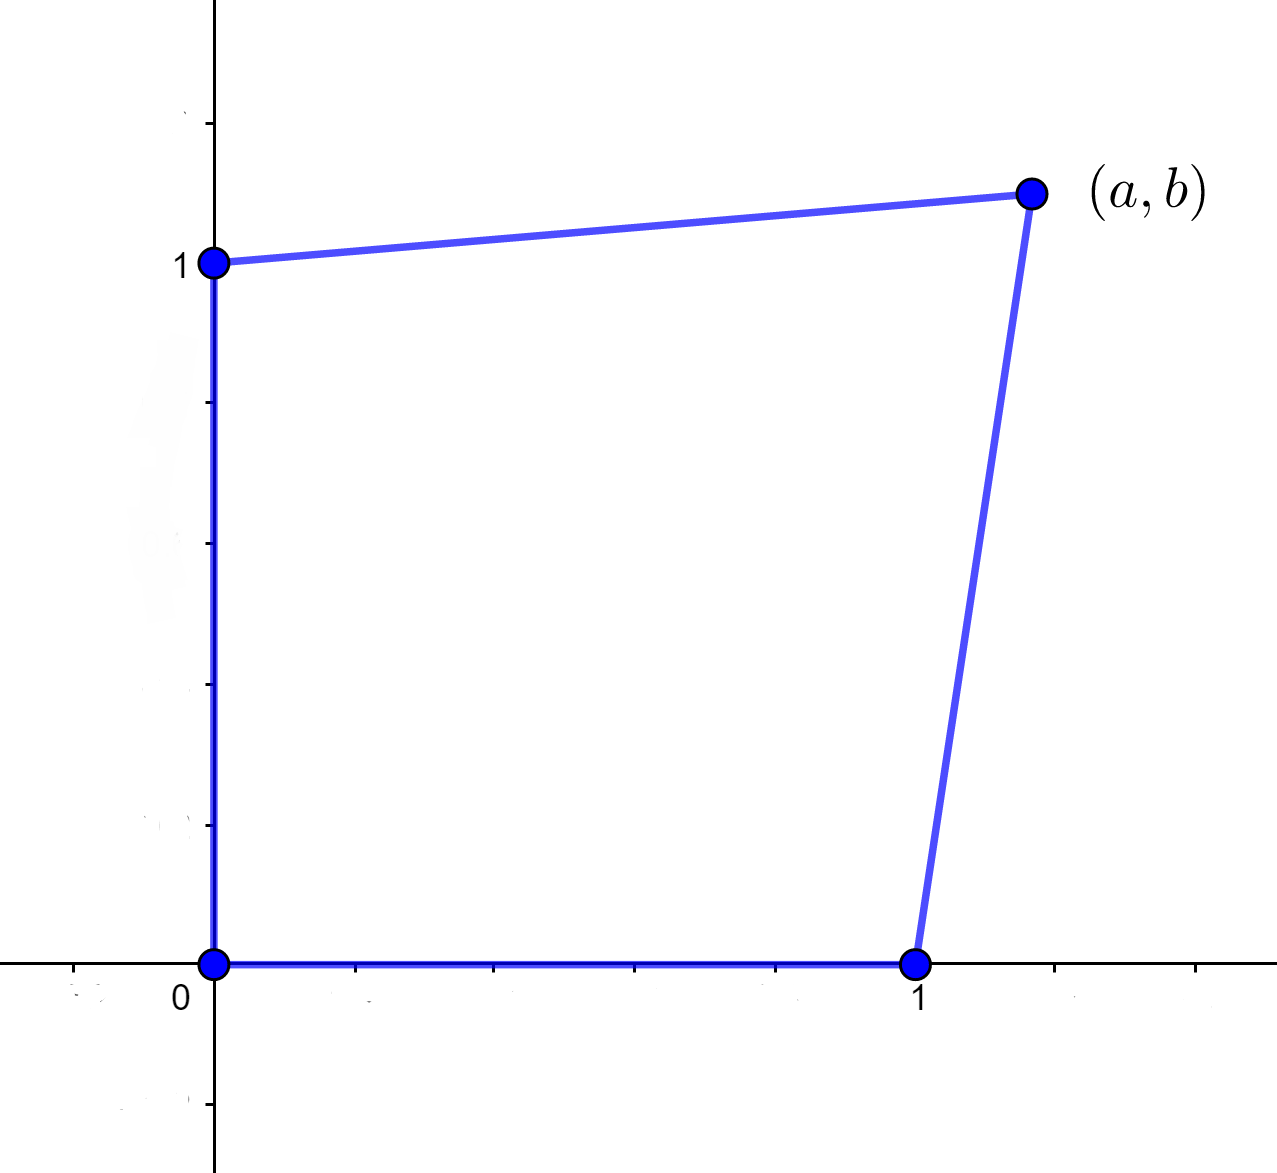
\includegraphics[width=0.35\linewidth]{pic22}
\end{figure}
\noindent
Рассмотрим пучок коник через точки $A_1 = (0,0),\ A_2 = (1,0),\ A_3 = (0,1),\ A_4 = (a,b)$, где $a,b > 0,\ a+b > 1$\\
\begin{gather*}
	C_1: x(x-a) = f(x,y)\\
	C_2: y(y-b) = g(x,y)
\end{gather*}
Пусть пятая точка имеет координаты $A_5 = (c,d)$\\
\begin{gather*}
	C_{A_5} f(A_5) g(A) - g(A_5) f(A) = x(x-a) d(d-b) - y(y-b) c(c-a)
\end{gather*}
Будем считать, что это было в карте $Z = 1$
\begin{gather*}
	\begin{pmatrix}
		0 & \ldots & \ldots\\
		\vdots & d(d-b) & 0\\
		\vdots & 0 & -c(c-a)
	\end{pmatrix}\\
	\\
	\text{det}
	\begin{pmatrix}
	d(d-b) & 0\\
	0 & -c(c-a)
	\end{pmatrix}
	=
	-d(d-b)c(c-a) = A
\end{gather*}
$A > 0$, если $d(d-b)c(c-a) < 0$, в этом случае коника -- эллипс
\begin{figure}[h!]
	\center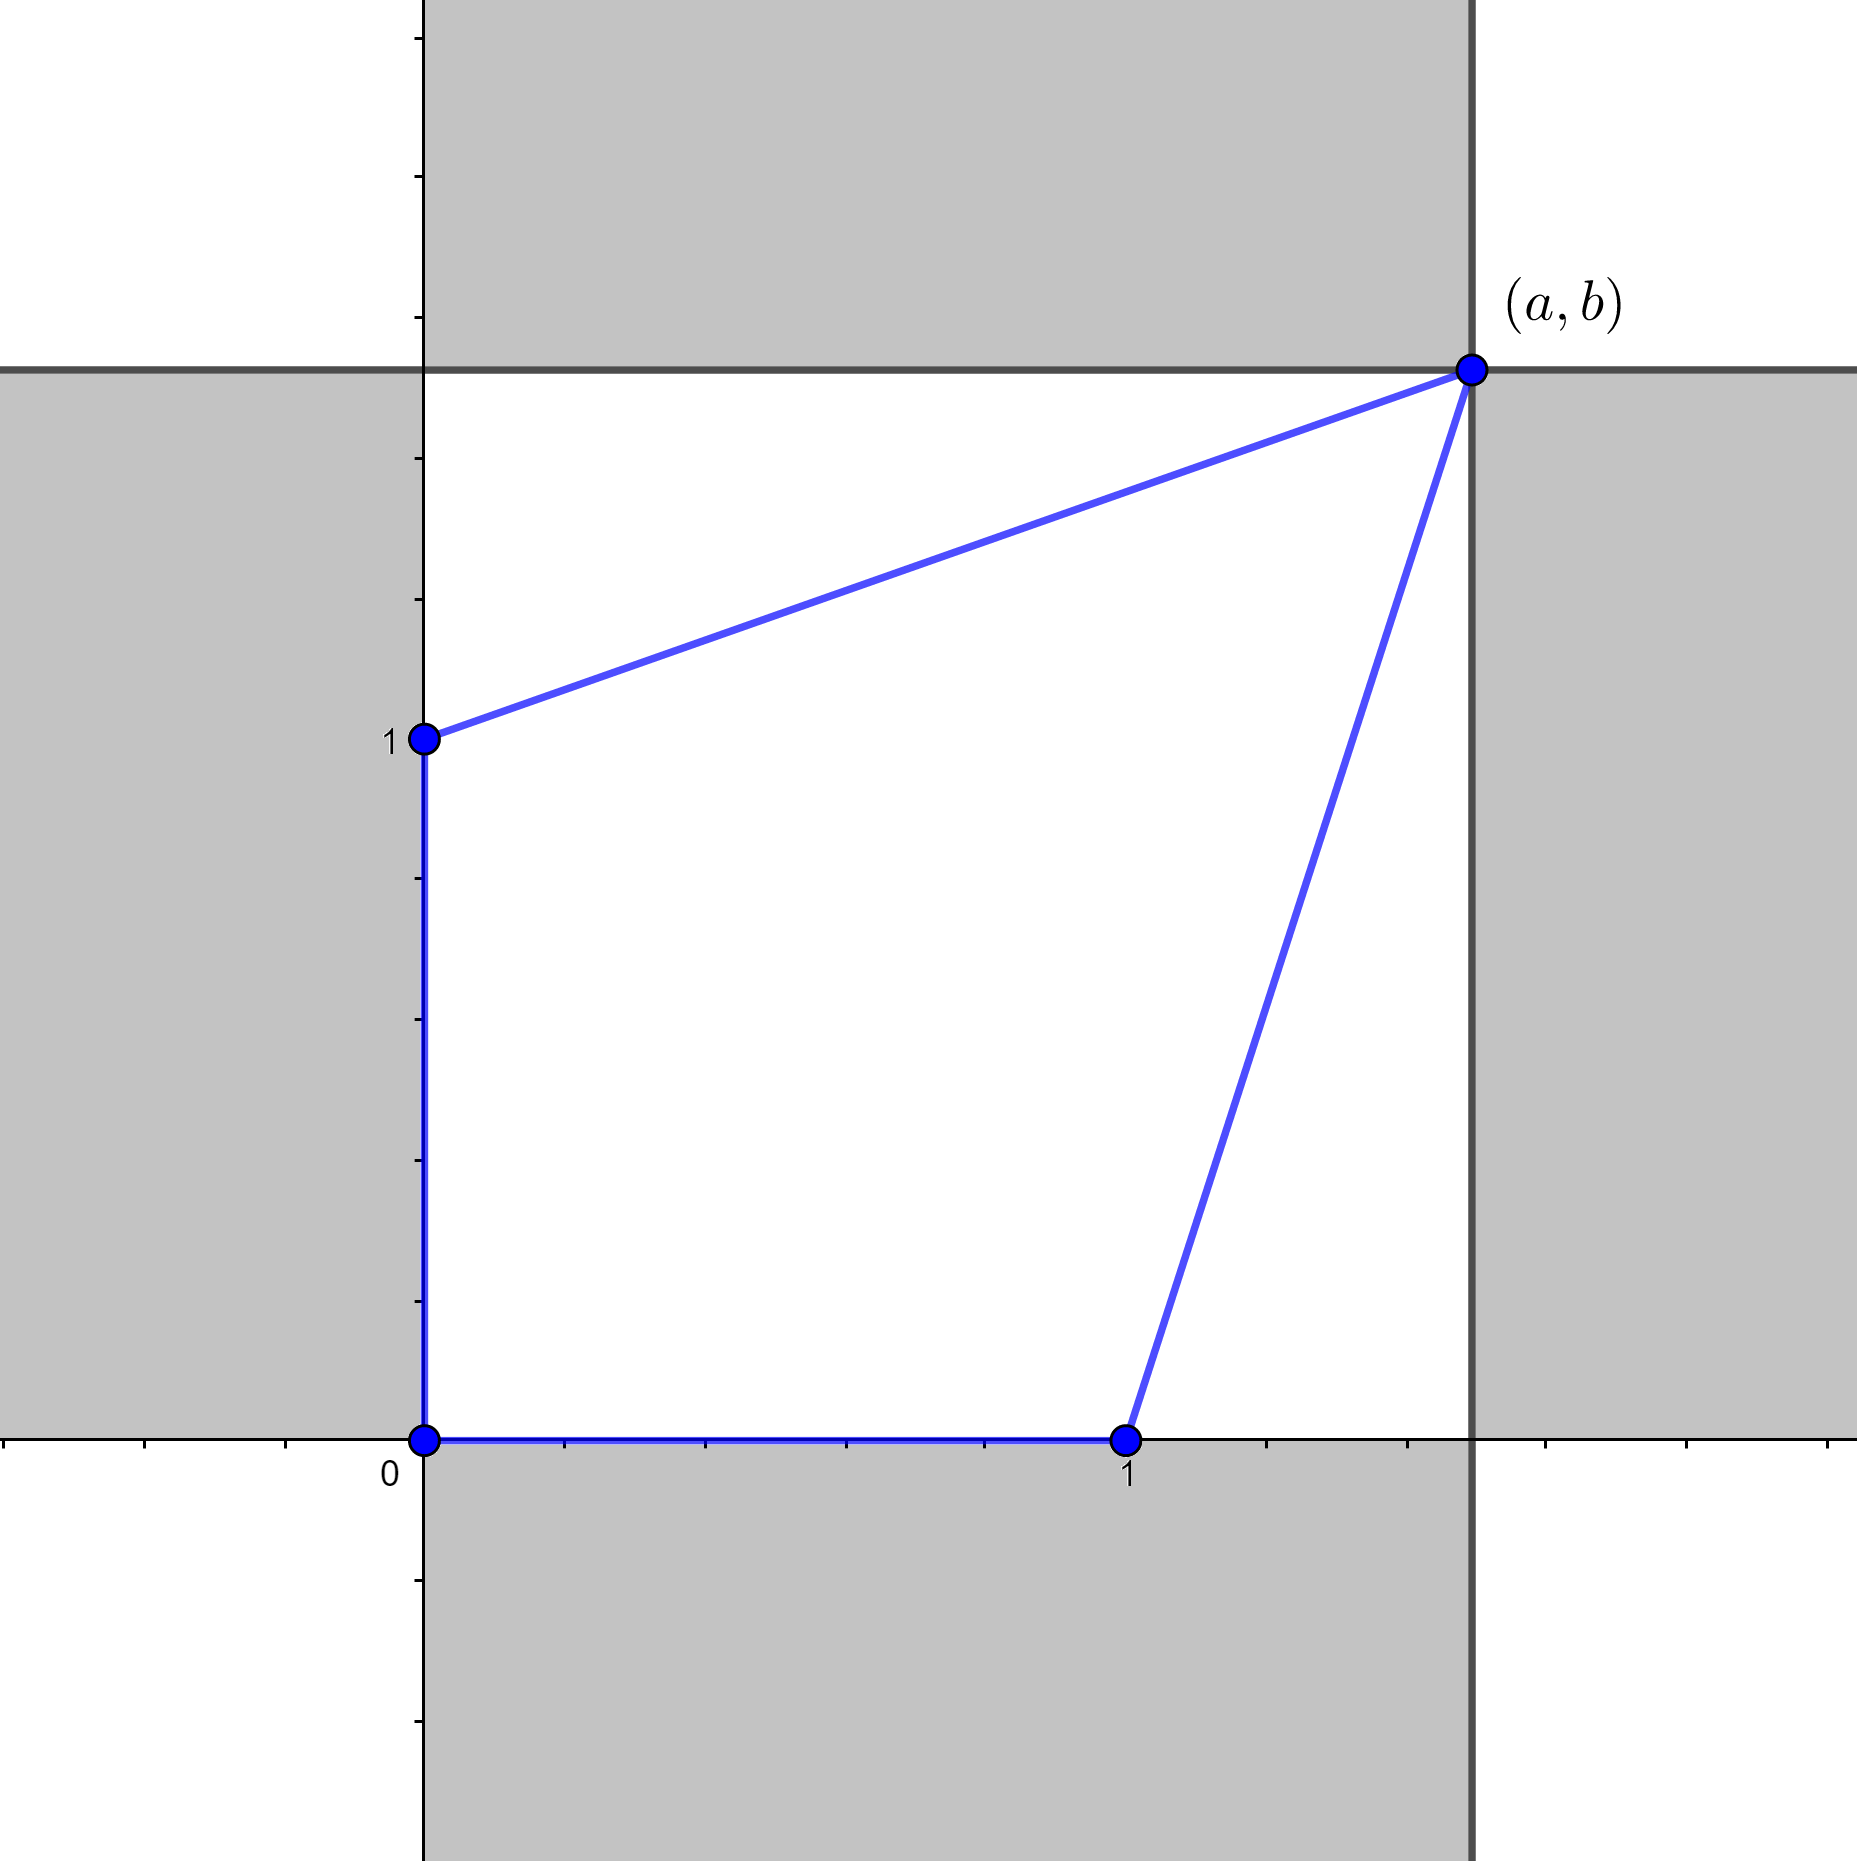
\includegraphics[width=0.35\linewidth]{pic23}
\end{figure} %+
	\subsection*{ГЛ7 5*}
Рассмотрим октаплекс $\{3,4,3\}$\\
\begin{enumerate}
\item[А] Известно, что $N_0 - N_1 + N_2 - N_3 = 0$\\
	У октаплекса 24 вершины (), ребер $\frac{24 \cdot 8}{2} = 96$ 
	\begin{gather*}
		\begin{matrix}
			\text{размерность} & \text{тип грани и ее количество}\\
			0 & 24\\
			1 & 96\\
			2 & 96\\
			3 & 24\\
			4 & 1
		\end{matrix}
	\end{gather*}
\item[Б] 
\item[В] Правильные октаэдры $\{3,4\}$
\item[Г] Правильные треугольники $\{3\}$

\end{enumerate}
		 %+
	\subsection*{ГЛ10 6}
$\text{sgn}(\text{tr}A^2)$
\begin{enumerate}
\item 
	разберем случай $\text{Mat}_2(\mathbb{R})$\\
	\begin{gather*}
		\text{tr}
		\begin{pmatrix}
			a_{11} & a_{12}\\
			a_{21} & a_{22}
		\end{pmatrix}^2 = a_{11}^2 + 2a_{12}a_{21} + a^2_{22}\\
		q = 
		\begin{pmatrix}
			1 & 0 & 0 & 0\\
			0 & 0 & 2 & 0\\
			0 & 2 & 0 & 0\\
			0 & 0 & 0 & 1						
		\end{pmatrix}
		\quad
		\begin{matrix}
			\Delta_1 > 0\\
			\Delta_2 = 0\\
			\Delta_3 < 0\\
			\Delta_4 < 0
		\end{matrix}
	\end{gather*}
\item 
	$\text{Mat}_{n}(\mathbb{R})$\\
	Всего $n^2$ элементов
	\begin{gather*}
		\text{tr}A^2 = \sum\limits^{n}_{i=1}a^2_{ii} + 2\sum\limits^{n}_{\substack{i<j \\ i = 1}}a_{ij}a_{ji}
	\end{gather*}
	Запишем матрицу грама, упорядочив столбцы по возрастанию суммы индексов:\\
	$a_{11},\ a_{12},\ a_{21},\ a_{22},\ a_{13},\ a_{31},\ a_{23},\ a_{32},\ a_{33},\ldots$\\
	Тогда матрица грама состоит из блоков 
	$\begin{pmatrix}
		0 & 2\\
		2 & 0
	\end{pmatrix} \simeq H^2$
	на диагонали и $1$ при $a_{ii}$\\
	Так как между $a_{k^2k^2}$ и $a_{(k+1)^2(k+1)^2}$ ровно $k$ гиперболических пространств, то $(p_{(k+1)^2-1}, m_{(k+1)^2-1}) = (p_{k^2}+k, m_{k^2}+k)$\\
	Так как знак $\Delta_{(k+1)^2}$ определяется суммой всех $H^2\ ((-1)^{\sum H^2})$, и $\Delta_{(k+1)^2} \cdot \Delta_{(k+1)^2-1} > 0$, следовательно $\text{sgn} = (p_{k^2}+k+1, m_{k^2}+k)$, откуда по индукции получаем:
	\begin{gather*}
		\Delta_{1} > 0\quad (1,0)\\
		\Delta_{2} = 0\\
		\Delta_{3} < 0\\
		\Delta_{4} < 0\quad (3,1)\\
		\Delta_{5} = 0\\
		\Delta_{6} > 0\\
		\Delta_{7} = 0\\
		\Delta_{8} < 0\\
		\Delta_{9} < 0\quad (6,3)\\
		\Delta_{10} = 0\\
		\Delta_{11} > 0\\
		\Delta_{12} = 0\\
		\Delta_{13} < 0\\
		\Delta_{14} = 0\\
		\Delta_{15} > 0\\
		\Delta_{16} > 0\quad (10,6)\\
	\end{gather*}
	Откуда: $\text{sgn}(1+2+\ldots+n, 1+2+\ldots+(n-1)) = \text{sgn}(\frac{1+n}{2}\cdot n, \frac{n}{2}(n-1))$
\end{enumerate}
		 %+
%	\subsection*{ГЛ14 7*}
Докажем задачу методом индукции.\\
Заметим, что при $n=2$ можно дополнить матрицу $D$ строкой единиц сверху, столбцом единиц слева и $0$ в верхнем левом углу и тогда определитель полученной матрицы будет эквивалентен формуле Герона.
\begin{gather*}
	\begin{vmatrix}
		0 & 1 & 1 & 1\\
		1 & 0 & d_{12}^2 & d_{13}^2\\
		1 & d_{12}^2 & 0 & d_{23}^2\\
		1 & d_{13}^2 & d_{23}^2 & 0
	\end{vmatrix}
	= d_{12}^4 + d_{13}^4 + d_{23}^4 + 2(d_{12}^2 d_{13}^2 + d_{12}^2 d_{23}^2 + d_{13}^2 d_{23}^2) =\\
	\\
	(-1)^{3}(d_{12}+d_{13}+d_{23})(d_{12}+d_{13}-d_{23})(d_{12}-d_{13}+d_{23})(-d_{12}+d_{13}+d_{23})\\
\end{gather*}
Откуда следует что он неотрицателен в случае когда треугольник с данными сторонами существует (в случае вырожденного треугольника определитель равен 0).\\
Тогда предположим что утверждение о существовании симплекса доказано для $n = 1, \ldots, k$, докажем тогда что утверждение выполнено и для $n = k+1$\\
Рассмотрим матрицу $D$ размера $(k+1) \times (k+1)$, тогда, по предположению индукции, мы знаем, что существуют $k$ мерные симплексы с вершинами $p_0, \ldots, p_{i-1}, p_{i+1}, \ldots, p_{k+1}$, так как для них выполнено утверждение. 
		
\newpage
{\large \hspace{3cm} \begin{center} Домашнее задание 23 $\bullet$ Мозговой Владислав \end{center} }
\vspace{-1.5ex}
\hrulefill
	
\fontsize{12pt}{4.5mm}\selectfont
\vspace{-3ex}
\hrulefill
\newline

\section*{}
	\subsection*{\textbf{Задача 1}}
	\textbf{Условие}\\
	Дана операция
	$
	A:=
	\begin{bmatrix}
		0 & -1 & 0 & 0 & 0 \\
		1 & -1 & 0 & 0 & 0 \\
		0 & 0 & 0 & 0 & -1 \\
		0 & 0 & 1 & 0 & 2 \\
		0 & 0 & 0 & 1 & 0
	\end{bmatrix}
	$
	Найдите $\text{tr}(A^{-2})$\\
	\\
	\textbf{Решение}
	\begin{gather*}
		\begin{bmatrix}
			0 & -1 & 0 & 0 & 0 \\
			1 & -1 & 0 & 0 & 0 \\
			0 & 0 & 0 & 0 & -1 \\
			0 & 0 & 1 & 0 & 2 \\
			0 & 0 & 0 & 1 & 0
		\end{bmatrix}
		^{-1}
		=
		\frac{1}{\text{det}(A)} A^{T}_{+}
		=
		-1 \cdot A^{T}_{+}
		=
		-A^{T}_{+}
		=
		\begin{bmatrix}
			-1 & 1 & 0 & 0 & 0 \\
			-1 & 0 & 0 & 0 & 0 \\
			0 & 0 & 2 & 1 & 0 \\
			0 & 0 & 0 & 0 & 1 \\
			0 & 0 & -1 & 0 & 0
		\end{bmatrix}
		\\
		\\
		\begin{bmatrix}
			0 & -1 & 0 & 0 & 0 \\
			1 & -1 & 0 & 0 & 0 \\
			0 & 0 & 0 & 0 & -1 \\
			0 & 0 & 1 & 0 & 2 \\
			0 & 0 & 0 & 1 & 0
		\end{bmatrix}
		^{-2}
		=
		\begin{bmatrix}
			-1 & 1 & 0 & 0 & 0 \\
			-1 & 0 & 0 & 0 & 0 \\
			0 & 0 & 2 & 1 & 0 \\
			0 & 0 & 0 & 0 & 1 \\
			0 & 0 & -1 & 0 & 0
		\end{bmatrix}
		^{2}
		=
		\begin{bmatrix}
			0 & -1 & 0 & 0 & 0 \\
			1 & -1 & 0 & 0 & 0 \\
			0 & 0 & 4 & 2 & 1 \\
			0 & 0 & -1 & 0 & 0 \\
			0 & 0 & -2 & -1 & 0
		\end{bmatrix}
		\\
		\\
		\text{tr}(A^{-2}) = (-1)^{2} + 4^{2} = 1 + 16 = 17
	\end{gather*}
	
	\newpage
	\subsection*{\textbf{Задача 2}}
	Известно, что суммы $i$-тых степеней корней многочлена $f(x)$ третьей степени $3,3$ и $3$ для $i = 1,2,4$ соответственно
	\subsubsection*{\textbf{А}}
	\textbf{Условие}\\
	Найдите $f(x)$\\
	\\
	\textbf{Решение}\\
	\begin{gather*}
		f(x) = (x - x_1)(x - x_2)(x - x_3)\\
		x_1 + x_2 + x_3 = 3\\
		x_1^{2} + x_2^{2} + x_3^{2} = (x_1 + x_2 + x_3)^2 - 2(x_1 x_2 + x_1 x_3 + x_2 x_3) = 3\\
		x_1^{4} + x_2^{4} + x_3^{4} = (x_1 + x_2 + x_3)^4 - 6(x_1 x_2 + x_1 x_3 + x_2 x_3)^{2}\\
		- 4(x_1 x_2 + x_1 x_3 + x_2 x_3)(x_1^2 + x_2^2 + x_2^3) + 4(x_1 + x_2 + x_3)x_1x_2x_3 = 3\\
		\\
		3^2 - 2(x_1 x_2 + x_1 x_3 + x_2 x_3) = 3\\
		x_1 x_2 + x_1 x_3 + x_2 x_3 = 3\\
		\\
		(x_1 + x_2 + x_3)^4 - 6(x_1 x_2 + x_1 x_3 + x_2 x_3)^{2}\\
		- 4(x_1 x_2 + x_1 x_3 + x_2 x_3)(x_1^2 + x_2^2 + x_2^3) + 4(x_1 + x_2 + x_3)x_1x_2x_3 = 3\\
		(x_1 + x_2 + x_3)^4 - 6(x_1 x_2 + x_1 x_3 + x_2 x_3)^{2}\\
		- 4(x_1 x_2 + x_1 x_3 + x_2 x_3)((x_1 + x_2 + x_3)^2 - 2(x_1 x_2 + x_1 x_3 + x_2 x_3)) + 4(x_1 + x_2 + x_3)x_1x_2x_3 = 3\\
		3^4 - 6 \cdot 3^{2} - 4 \cdot 3 \cdot 3 + 4 \cdot 3  \cdot x_1x_2x_3 = 3\\
		81 - 54 - 36 + 12 x_1x_2x_3 = 3\\
		12 x_1x_2x_3 = 12\\
		x_1x_2x_3 = 1\\
		\\
		f(x) = x^3 - 3x^2 + 3x - 1 = (x-1)^{3}
	\end{gather*}
	
	\subsubsection*{\textbf{Б}}
	\textbf{Условие}\\
	Найдите суммы 5-ых степеней корней многочлена $f(x)$\\
	\\
	\textbf{Решение}\\
	\begin{gather*}
		f(x) = x^3 - 3x^2 + 3x - 1 = (x-1)^{3}\\
		x_1^5 + x_2^5 + x_3^5 = (x_1 + x_2 + x_3)^5 - 5(x_1^3 + x_2^3 + x_3^3)(x_1x_2 + x_1x_3 + x_2x_3)\\
		- 20x_1x_2x_3(x_1x_2 + x_1x_3 + x_2x_3) - 15(x_1^2 + x_2^2 + x_3^2)x_1x_2x_3 -10(x_1 + x_2 + x_3)(x_1^2 x_2^2 + x_1^2 x_3^2 + x_2^2 x_3^2)\\
		\\
		x_1^5 + x_2^5 + x_3^5 =\\
		(x_1 + x_2 + x_3)^5 - 5((x_1 + x_2 + x_3)^3 - 3(x_1+x_2+x_3)(x_1x_2+x_1x_3+x_2x_3) + 3x_1x_2x_3) \cdot \\
		(x_1x_2 + x_1x_3 + x_2x_3) - 20x_1x_2x_3(x_1x_2 + x_1x_3 + x_2x_3)\\
		- 15((x_1 + x_2 + x_3)^2 - 2(x_1 x_2 + x_1 x_3 + x_2 x_3))x_1x_2x_3\\
		- 10(x_1 + x_2 + x_3)((x_1x_2 + x_1x_3 + x_2x_3)^2 - 2x_1x_2x_3(x_1+x_2+x_3))\\
		\\
		1^5 + 1^5 + 1^5 = 3
	\end{gather*}
	
	\newpage
	\subsection*{\textbf{Задача 3}}
	\subsubsection*{\textbf{А}}
	\textbf{Условие}\\
	Пусть многочлены $A(x), B(x)$ -- многочлены с коэффициентами в поле, со страшим коэффициентом 1, и пусть $Q(x)$ -- остаток от деления $B(x)$ на $A(X)$. Покажите что результанты многочленов $A(x)$ и $B(x)$ и многочленов $A(x)$ и $Q(x)$ совпадают.\\
	\\
	\textbf{Решение}\\
	\begin{gather*}
		A(x) = x^{n} + a_{n-1}x^{n-1} + \ldots + a_1\\
		B(x) = x^{m} + b_{m-1}x^{m-1} + \ldots + b_1\\
		Q(x) = x^{k} + q_{k-1}x^{k-1} + \ldots + q_1\\
		B = AS + Q\quad S \text{ -- какой-то многочлен}\\
		S(x) = x^{l} + s_{l-1}x^{l-1} + \ldots + a_1\\
		\\
		AS = S_0A + S_1xA + \ldots + x^{l} A
	\end{gather*}
	При умножении $A$ на $x_i$ коэффициенты будут смещаться на $i$ так как
	\begin{gather*}
		x^{i} A = x^{n+i} + a_{n-1+i} x^{n-1+i} + \ldots + a_{0 + i} x^{i}
	\end{gather*}
	Следовательно домножение $A$ на $x^{i}$ происходит элементарное преобразование строк, а следовательно дискриминант не изменяется.\\
	Откуда следует, что так как $-SA + B$ -- результат элементарных преобразований, то
	\begin{gather*}
		R(A,B) = R(-SA+B, B) = R(Q,B)
	\end{gather*}
	
	\newpage
	\subsubsection*{\textbf{Б}}
	\textbf{Условие}\\
	Вычислите дискриминант многочлена $x^8 + ax + b$ и выясните при каких $a,b \in \mathbb{F}_{7}$ многочлен $x^{8} + ax + b$ делится на квадрат неприводимого многочлена над $\mathbb{F}_{7}$?\\
	\\
	\textbf{Решение}
	\begin{gather*}
		f'(x) = 8x^7 + a\\
		D = a_{0}^{2n-2} \prod_{i<j}(a_i - a_j)^{2}\\
		R(f,f')= (-1)^{\frac{n(n-1)}{2}}a_{0}D\\
		\\
		R(f,f') = 
		\left|
		\begin{array}{ccccccccccccccc}
			1 & 0 & 0 & 0 & 0 & 0 & 0 & a & b & 0 & 0 & 0 & 0 & 0 & 0 \\
			0 & 1 & 0 & 0 & 0 & 0 & 0 & 0 & a & b & 0 & 0 & 0 & 0 & 0 \\
			0 & 0 & 1 & 0 & 0 & 0 & 0 & 0 & 0 & a & b & 0 & 0 & 0 & 0 \\
			0 & 0 & 0 & 1 & 0 & 0 & 0 & 0 & 0 & 0 & a & b & 0 & 0 & 0 \\
			0 & 0 & 0 & 0 & 1 & 0 & 0 & 0 & 0 & 0 & 0 & a & b & 0 & 0 \\
			0 & 0 & 0 & 0 & 0 & 1 & 0 & 0 & 0 & 0 & 0 & 0 & a & b & 0 \\
			0 & 0 & 0 & 0 & 0 & 0 & 1 & 0 & 0 & 0 & 0 & 0 & 0 & a & b \\
			8 & 0 & 0 & 0 & 0 & 0 & 0 & a & 0 & 0 & 0 & 0 & 0 & 0 & 0 \\
			0 & 8 & 0 & 0 & 0 & 0 & 0 & 0 & a & 0 & 0 & 0 & 0 & 0 & 0 \\
			0 & 0 & 8 & 0 & 0 & 0 & 0 & 0 & 0 & a & 0 & 0 & 0 & 0 & 0 \\
			0 & 0 & 0 & 8 & 0 & 0 & 0 & 0 & 0 & 0 & a & 0 & 0 & 0 & 0 \\
			0 & 0 & 0 & 0 & 8 & 0 & 0 & 0 & 0 & 0 & 0 & a & 0 & 0 & 0 \\
			0 & 0 & 0 & 0 & 0 & 8 & 0 & 0 & 0 & 0 & 0 & 0 & a & 0 & 0 \\
			0 & 0 & 0 & 0 & 0 & 0 & 8 & 0 & 0 & 0 & 0 & 0 & 0 & a & 0 \\
			0 & 0 & 0 & 0 & 0 & 0 & 0 & 8 & 0 & 0 & 0 & 0 & 0 & 0 & a
		\end{array}
		\right|
		=
		8^{8}b^7 - 7^{7} a^8\\
		\\
		D = \frac{R(f,f')}{(-1)^{\frac{n(n-1)}{2}} a_0} = \frac{8^{8}b^7 - 7^{7} a^8}{(-1)^{\frac{8(8-1)}{2}} \cdot 1} = 8^{8}b^7 - 7^{7} a^8
	\end{gather*}
	Рассмотрим неприводимый многочлен $A = x^n + a_{n-1} x^n + \ldots + a_{0},\ \forall i:\ a_i \in \mathbb{F}_7$. По основной теореме алгебры он имеет минимум один корень над $\mathbb{C}$, тогда $A = \prod_{i = 1} (x - x_i)^{k_i},\ A^2 = \prod_{i = 1} (x - x_i)^{2k_i}$, то есть имеет кратные корни. Следовательно если $x^8 + ax + b$ делится на $A^2$, то $D(A) = 0$.
	$D(A) = 8^8b^7 - 7^7a^8 \equiv 6b^7 = 0$, а следовательно $b = 0$, $a$ -- любое.\\

	
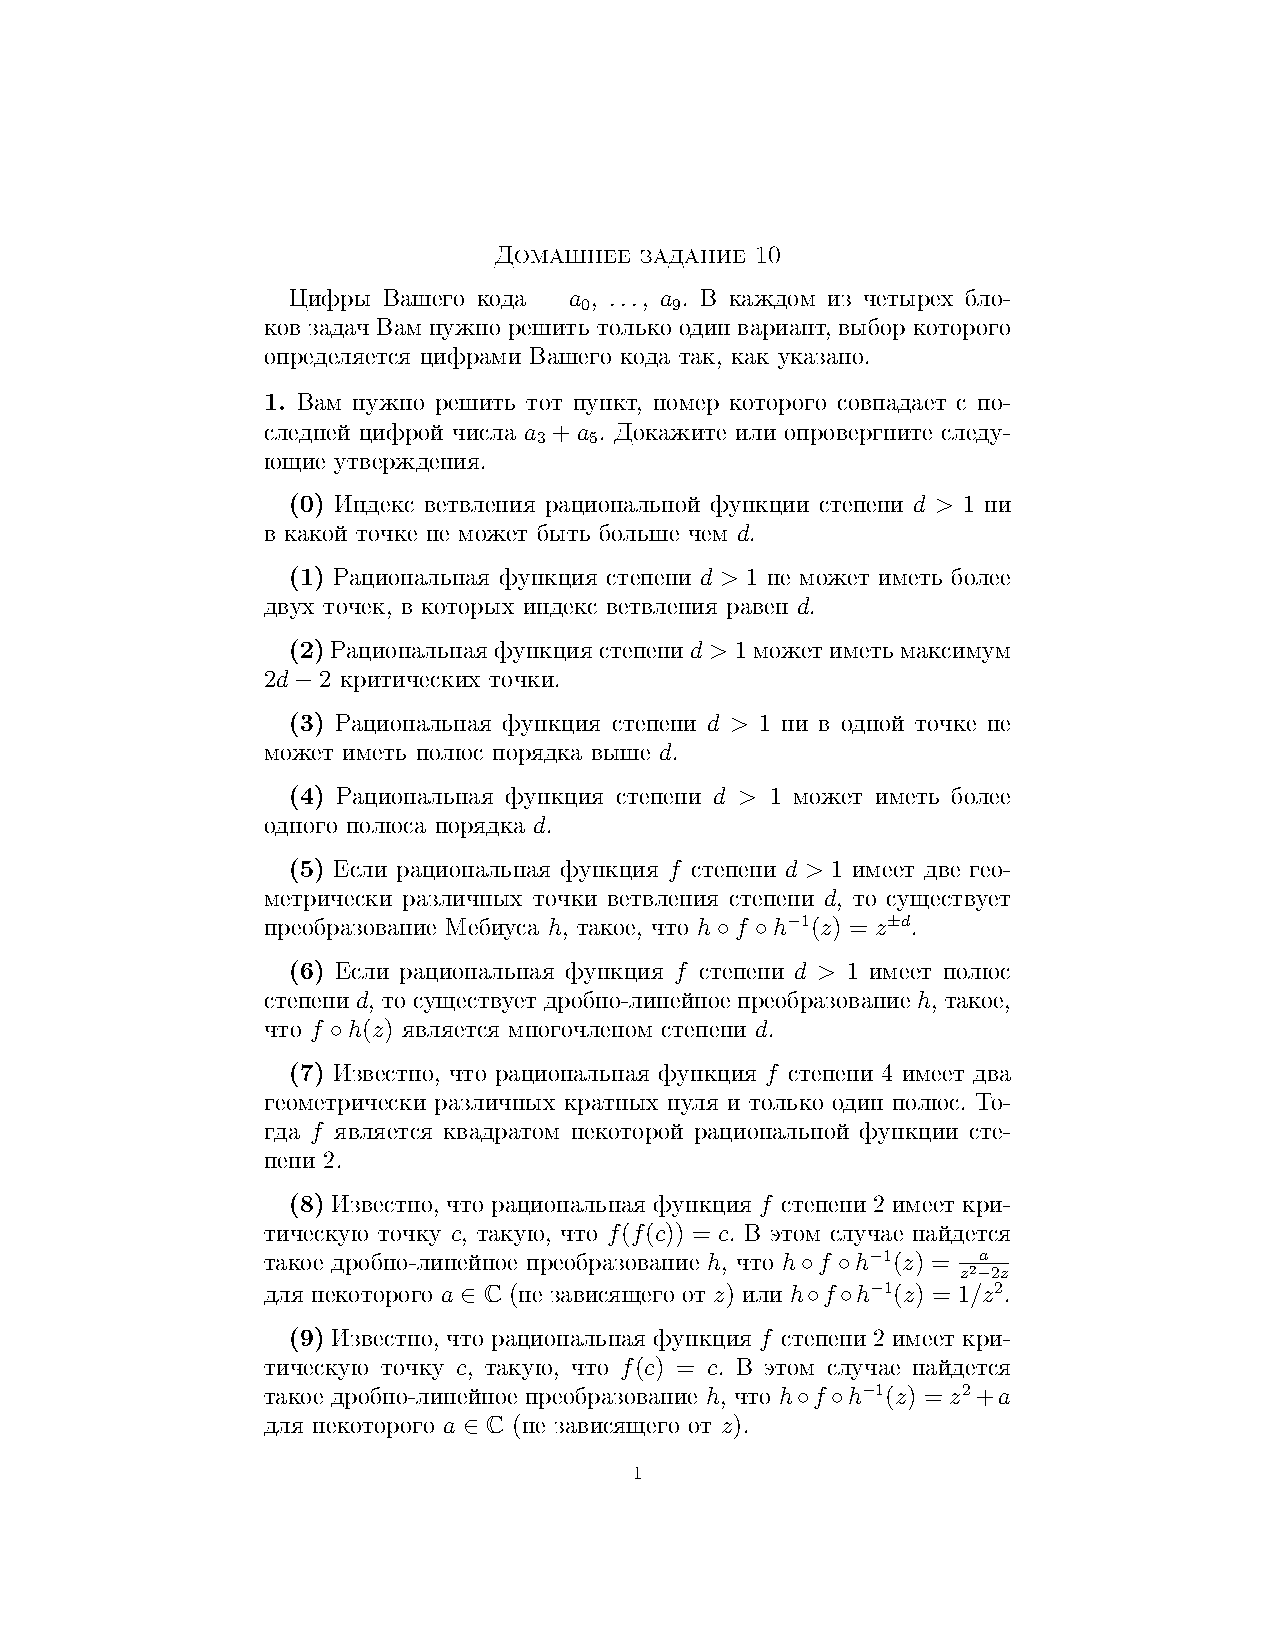
\includepdf[scale=1,pages=1-4]{Tasks/hw10}
\newpage
\section*{Решения}
\subsection*{Задача 1}
	Необходимо решить задачу $a_3 + a_5 = 9 + 6 = 5 \mod 10$\\
	5 задача оказалась сложной, поэтому я записал 4\\
	Заметим что рациональную функцию можно представить в виде $\frac{p(z)}{q(z)}$, допустим что у рассматриваемой функции есть хотя бы 2 полюса степени $d$, назовем их $z_1,\ z_2$. Тогда функцию можно представить как $\frac{p(z)}{(z - z_1)^d (z - z_2)^d q_1(z)}$, $(z - z_1)^d (z - z_2)^d q_1(z) = q(z)$, тогда $\deg((z - z_1)^d (z - z_2)^d q_1(z)) \geqslant 2d$, но $\deg(q(z)) \leqslant d$, противоречие.
\vskip 0.4in

\subsection*{Задача 2}
	Необходимо решить задачу $a_4 + a_6 = 7 + 9 = 6 \mod 10$\\
	\begin{gather*}
		a:\ z \mapsto \frac{z|z|}{1+|z|}\\
		P:\ z \mapsto z^2\\
		b:\ \text{id}\\
		a \circ P \circ b = \frac{z^2|z|^2}{1+|z|^2}
	\end{gather*}
\vskip 0.4in

\subsection*{Задача 3}
	Необходимо решить задачу $a_1 + a_5 = 7 + 6 = 3 \mod 10$\\
	Заметим что $f$ голоморфна, а следовательно аналитична, откуда следует что так как $\mathbb{D} \subset \mathbb{C}$ открыто, то $f(\mathbb{D})$ либо открыта в $\mathbb{C}$, либо константа, рассмотрим $f(z) = C$, $\Re(f(\mathbb{D})) = \Re(C) = \Re(a + bi) = a$, а точка не является открытым множеством
\vskip 0.4in

\subsection*{Задача 4}
	Необходимо решить задачу $a_0 + a_7 = 1 + 3 = 4 \mod 10$\\
	Заметим что функция $\sinh (ax)$ симметрична относительна начала координат
	\begin{gather*}
		\int_{\gamma_{R}} \frac{\sinh (a z) e^{i t z}}{\sinh (b z)} d z=2 \pi i \sum_{1 \leq n \leq R b / \pi} \operatorname{Res}\left(\frac{\sinh (a z) e^{i t z}}{\sinh (b z)}, \frac{\pi i n}{b}\right)\\
	\end{gather*}
	Где $\gamma_{R}$ -- замкнутый контур, состоящий из полуокружности радиуса $R$ и интервала $[-R,R]$, рассмотрев $R \to +\infty$ получим:
	\begin{gather*}
		\int_{-\infty}^{+\infty} \frac{\sinh (a x)}{\sinh (b x)} e^{i t x} d x
		= 2 \pi i \sum_{n=1}^{\infty} \operatorname{Res}\left(\frac{\sinh (a z) e^{i t z}}{\sinh (b z)}, \frac{\pi i n}{b}\right) \\
		= \frac{2 \pi i}{b} \sum_{n=1}^{\infty} \frac{\sinh (a \pi i n / b) e^{-\pi n t / b}}{\cosh (\pi i n)}
		= -\frac{2 \pi}{b} \sum_{n=1}^{\infty}(-1)^{n} \sin (a \pi n / b) e^{-\pi n t / b} \\
		= -\frac{2 \pi}{b} \operatorname{Im}\left(\sum_{n=1}^{\infty}(-1)^{n} e^{\pi n(-t+i a) / b}\right)
		= -\frac{2 \pi}{b} \operatorname{Im}\left(\frac{1}{1+e^{\pi(i a+t) / b}}\right)
	\end{gather*}
	Тогда рассмотрим $t \to 0^{+}$
	\begin{gather*}
		\int_{0}^{\infty} \frac{\sinh(ax)}{\sinh(bx)}dx = \frac{\pi}{2b} \cdot \frac{\sin(a\pi / b)}{\cos(a\pi /b) + 1}
	\end{gather*}
	Откуда при $b = \pi$ получаем
	\begin{gather*}
		\frac{\pi}{2b} \cdot \frac{\sin(a\pi / b)}{\cos(a\pi /b) + 1}
		= \frac{1}{2} \cdot \frac{\sin(a)}{\cos(a) + 1}
		= \frac{1}{2}\tan \frac{a}{2}
	\end{gather*}
\newpage		
	\section{Проективная геометрия}
	\subsection*{ГЛ10 1}
		 %+
	\subsection*{ГЛ9 2}
a) по задаче 6\\
б)\\
\\
в) %+
	\subsection*{ГЛ14 3}
\begin{enumerate}
	\item[(а)] 
	Вспомним задачу ГЛ$13\ 10$ про поиск ГМТ точек из которых эллипс виден под углом $90^{\circ}$. Там было доказано что длины диагонали описанного вокруг эллипса прямоугольника постоянна, а также был описан director circle данного эллипса, что является решением данной задачи при $n = 2$. Заметим что если выбрать какой-то базис и рассмотреть проекции диагонали на плоскости $x = 0,\ y = 0,\ z = 0$, то проекции будут иметь постоянную длину(так как проекция эллипсойда -- эллипс), а следовательно и длина самой диагонали тоже сохранится.
	\item[(б*)] 
\end{enumerate}
		 %+
%	\subsection*{ГЛ13 4}
\begin{figure}[h!]
	\center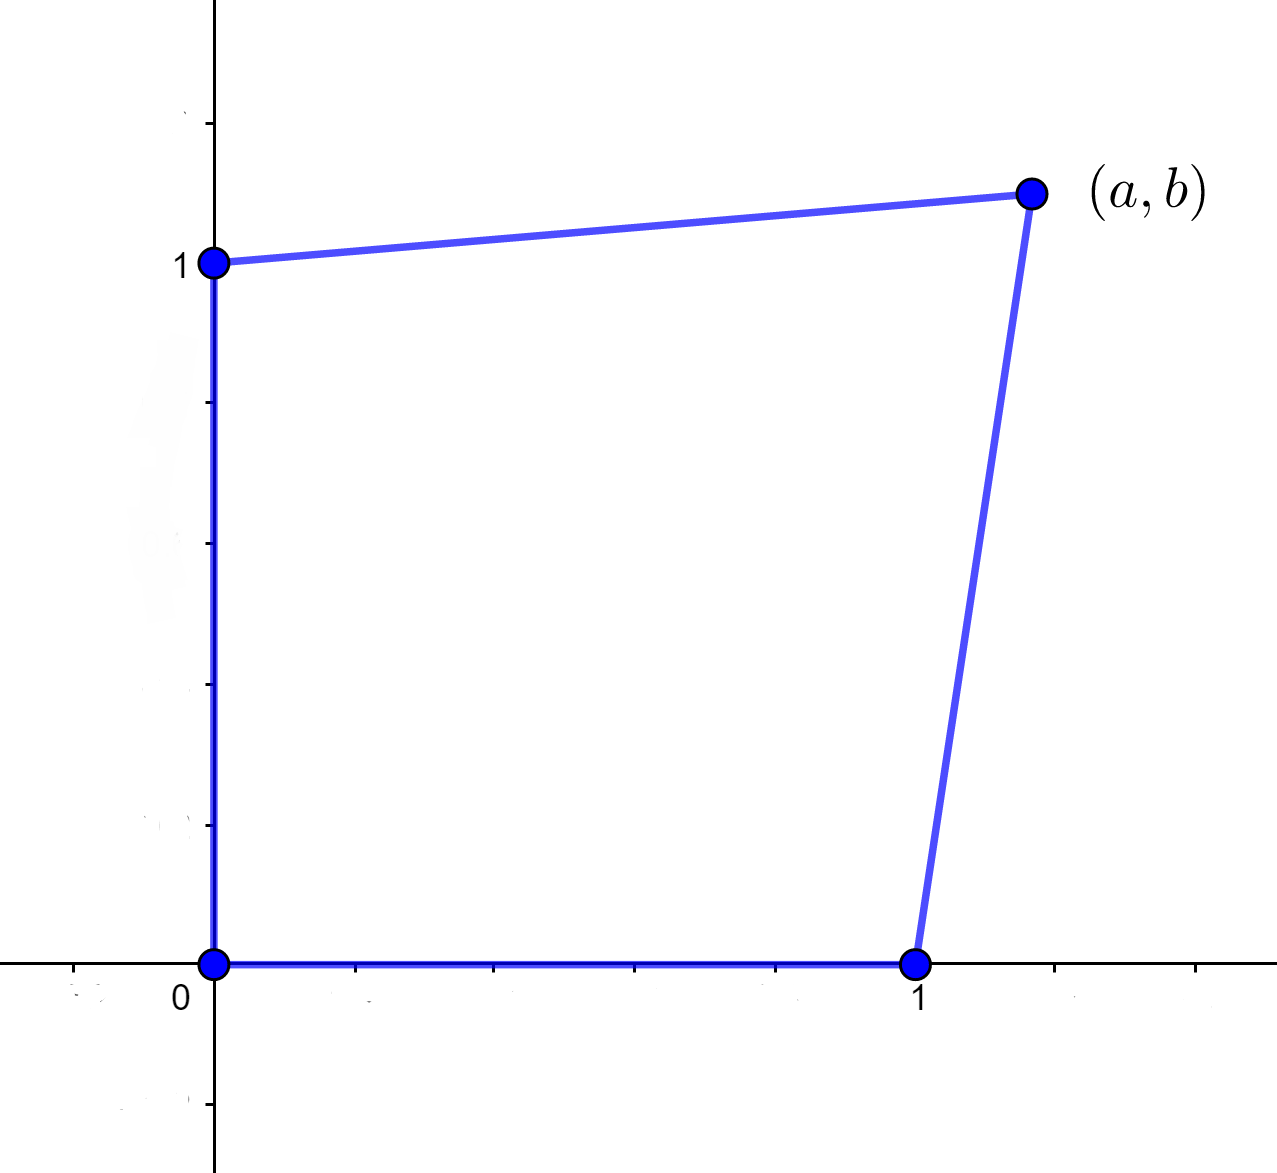
\includegraphics[width=0.35\linewidth]{pic22}
\end{figure}
\noindent
Рассмотрим пучок коник через точки $A_1 = (0,0),\ A_2 = (1,0),\ A_3 = (0,1),\ A_4 = (a,b)$, где $a,b > 0,\ a+b > 1$\\
\begin{gather*}
	C_1: x(x-a) = f(x,y)\\
	C_2: y(y-b) = g(x,y)
\end{gather*}
Пусть пятая точка имеет координаты $A_5 = (c,d)$\\
\begin{gather*}
	C_{A_5} f(A_5) g(A) - g(A_5) f(A) = x(x-a) d(d-b) - y(y-b) c(c-a)
\end{gather*}
Будем считать, что это было в карте $Z = 1$
\begin{gather*}
	\begin{pmatrix}
		0 & \ldots & \ldots\\
		\vdots & d(d-b) & 0\\
		\vdots & 0 & -c(c-a)
	\end{pmatrix}\\
	\\
	\text{det}
	\begin{pmatrix}
	d(d-b) & 0\\
	0 & -c(c-a)
	\end{pmatrix}
	=
	-d(d-b)c(c-a) = A
\end{gather*}
$A > 0$, если $d(d-b)c(c-a) < 0$, в этом случае коника -- эллипс
\begin{figure}[h!]
	\center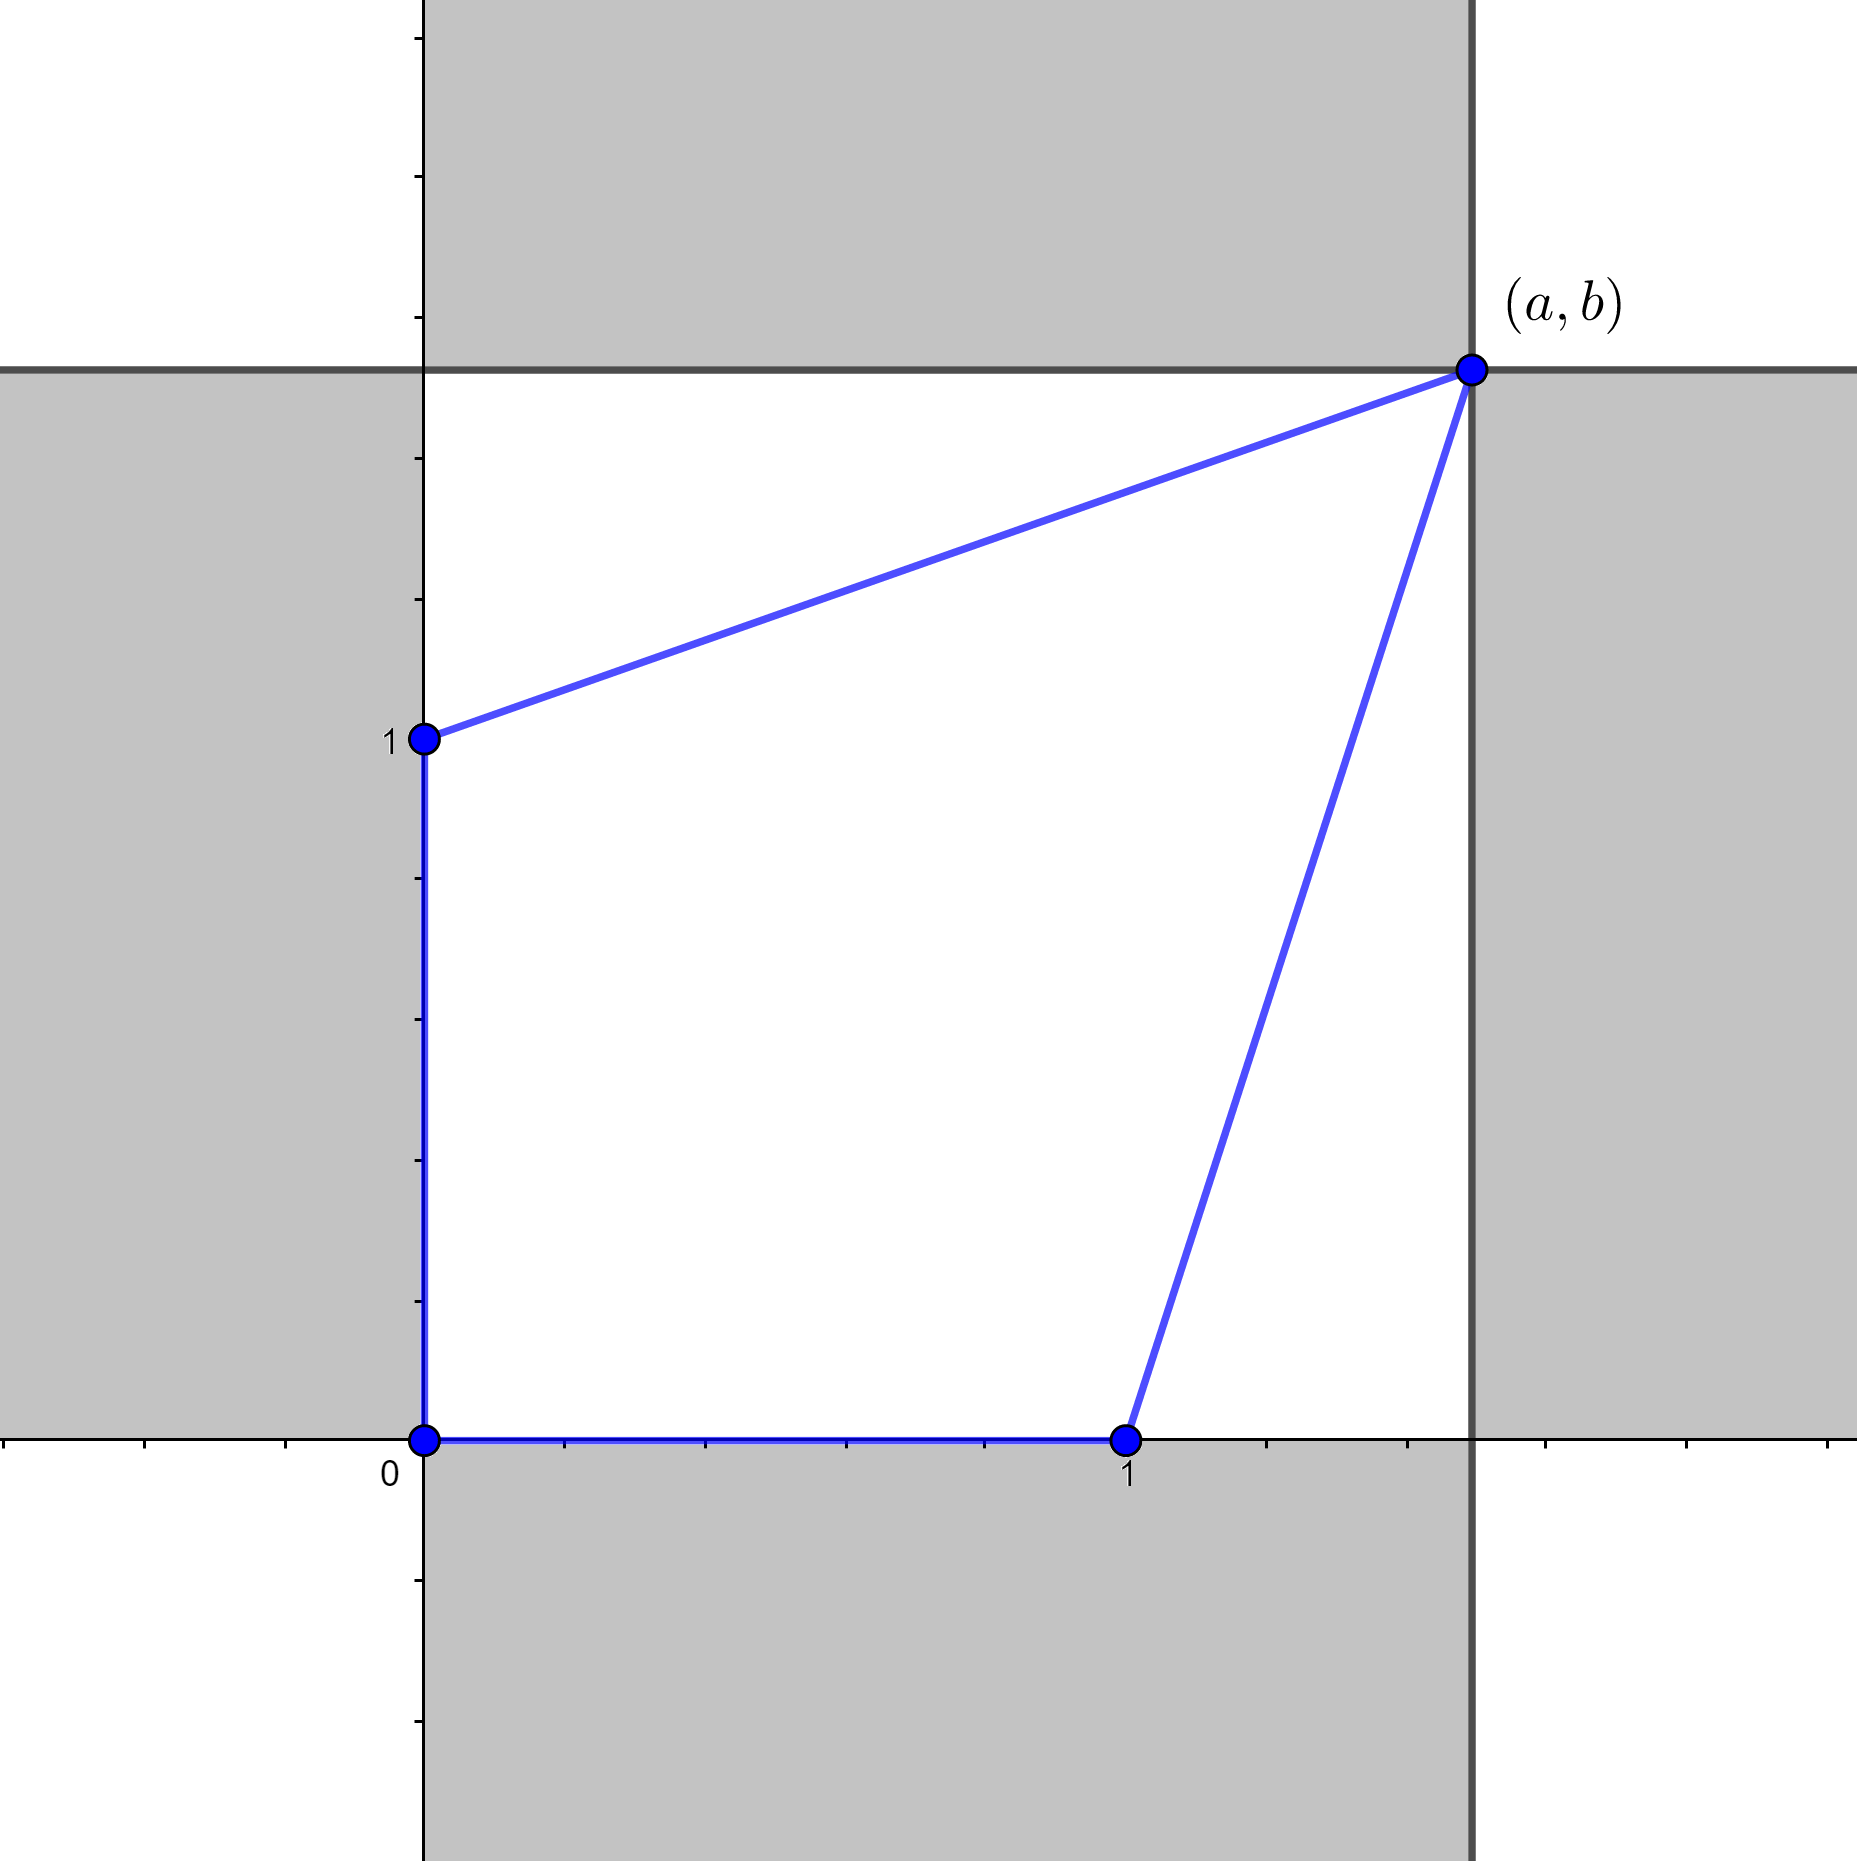
\includegraphics[width=0.35\linewidth]{pic23}
\end{figure}
	\subsection*{ГЛ7 5*}
Рассмотрим октаплекс $\{3,4,3\}$\\
\begin{enumerate}
\item[А] Известно, что $N_0 - N_1 + N_2 - N_3 = 0$\\
	У октаплекса 24 вершины (), ребер $\frac{24 \cdot 8}{2} = 96$ 
	\begin{gather*}
		\begin{matrix}
			\text{размерность} & \text{тип грани и ее количество}\\
			0 & 24\\
			1 & 96\\
			2 & 96\\
			3 & 24\\
			4 & 1
		\end{matrix}
	\end{gather*}
\item[Б] 
\item[В] Правильные октаэдры $\{3,4\}$
\item[Г] Правильные треугольники $\{3\}$

\end{enumerate}
		 %+
	\subsection*{ГЛ10 6}
$\text{sgn}(\text{tr}A^2)$
\begin{enumerate}
\item 
	разберем случай $\text{Mat}_2(\mathbb{R})$\\
	\begin{gather*}
		\text{tr}
		\begin{pmatrix}
			a_{11} & a_{12}\\
			a_{21} & a_{22}
		\end{pmatrix}^2 = a_{11}^2 + 2a_{12}a_{21} + a^2_{22}\\
		q = 
		\begin{pmatrix}
			1 & 0 & 0 & 0\\
			0 & 0 & 2 & 0\\
			0 & 2 & 0 & 0\\
			0 & 0 & 0 & 1						
		\end{pmatrix}
		\quad
		\begin{matrix}
			\Delta_1 > 0\\
			\Delta_2 = 0\\
			\Delta_3 < 0\\
			\Delta_4 < 0
		\end{matrix}
	\end{gather*}
\item 
	$\text{Mat}_{n}(\mathbb{R})$\\
	Всего $n^2$ элементов
	\begin{gather*}
		\text{tr}A^2 = \sum\limits^{n}_{i=1}a^2_{ii} + 2\sum\limits^{n}_{\substack{i<j \\ i = 1}}a_{ij}a_{ji}
	\end{gather*}
	Запишем матрицу грама, упорядочив столбцы по возрастанию суммы индексов:\\
	$a_{11},\ a_{12},\ a_{21},\ a_{22},\ a_{13},\ a_{31},\ a_{23},\ a_{32},\ a_{33},\ldots$\\
	Тогда матрица грама состоит из блоков 
	$\begin{pmatrix}
		0 & 2\\
		2 & 0
	\end{pmatrix} \simeq H^2$
	на диагонали и $1$ при $a_{ii}$\\
	Так как между $a_{k^2k^2}$ и $a_{(k+1)^2(k+1)^2}$ ровно $k$ гиперболических пространств, то $(p_{(k+1)^2-1}, m_{(k+1)^2-1}) = (p_{k^2}+k, m_{k^2}+k)$\\
	Так как знак $\Delta_{(k+1)^2}$ определяется суммой всех $H^2\ ((-1)^{\sum H^2})$, и $\Delta_{(k+1)^2} \cdot \Delta_{(k+1)^2-1} > 0$, следовательно $\text{sgn} = (p_{k^2}+k+1, m_{k^2}+k)$, откуда по индукции получаем:
	\begin{gather*}
		\Delta_{1} > 0\quad (1,0)\\
		\Delta_{2} = 0\\
		\Delta_{3} < 0\\
		\Delta_{4} < 0\quad (3,1)\\
		\Delta_{5} = 0\\
		\Delta_{6} > 0\\
		\Delta_{7} = 0\\
		\Delta_{8} < 0\\
		\Delta_{9} < 0\quad (6,3)\\
		\Delta_{10} = 0\\
		\Delta_{11} > 0\\
		\Delta_{12} = 0\\
		\Delta_{13} < 0\\
		\Delta_{14} = 0\\
		\Delta_{15} > 0\\
		\Delta_{16} > 0\quad (10,6)\\
	\end{gather*}
	Откуда: $\text{sgn}(1+2+\ldots+n, 1+2+\ldots+(n-1)) = \text{sgn}(\frac{1+n}{2}\cdot n, \frac{n}{2}(n-1))$
\end{enumerate}
		 %+
	\subsection*{ГЛ14 7*}
Докажем задачу методом индукции.\\
Заметим, что при $n=2$ можно дополнить матрицу $D$ строкой единиц сверху, столбцом единиц слева и $0$ в верхнем левом углу и тогда определитель полученной матрицы будет эквивалентен формуле Герона.
\begin{gather*}
	\begin{vmatrix}
		0 & 1 & 1 & 1\\
		1 & 0 & d_{12}^2 & d_{13}^2\\
		1 & d_{12}^2 & 0 & d_{23}^2\\
		1 & d_{13}^2 & d_{23}^2 & 0
	\end{vmatrix}
	= d_{12}^4 + d_{13}^4 + d_{23}^4 + 2(d_{12}^2 d_{13}^2 + d_{12}^2 d_{23}^2 + d_{13}^2 d_{23}^2) =\\
	\\
	(-1)^{3}(d_{12}+d_{13}+d_{23})(d_{12}+d_{13}-d_{23})(d_{12}-d_{13}+d_{23})(-d_{12}+d_{13}+d_{23})\\
\end{gather*}
Откуда следует что он неотрицателен в случае когда треугольник с данными сторонами существует (в случае вырожденного треугольника определитель равен 0).\\
Тогда предположим что утверждение о существовании симплекса доказано для $n = 1, \ldots, k$, докажем тогда что утверждение выполнено и для $n = k+1$\\
Рассмотрим матрицу $D$ размера $(k+1) \times (k+1)$, тогда, по предположению индукции, мы знаем, что существуют $k$ мерные симплексы с вершинами $p_0, \ldots, p_{i-1}, p_{i+1}, \ldots, p_{k+1}$, так как для них выполнено утверждение.  %+
	\subsection*{ГЛ10 8}
$f: \Omega_{2n} \simeq \Omega_{2n}$\\
Симплек. группа $\text{Sp}(\Omega_{2n})$
\begin{gather*}
	\text{Sp}_{2n}(k) = \{F \in \text{Mat}_{2n}(k)\ |\ F^t IF = I\}\quad I = 
	\begin{pmatrix}
		0 & E\\
		-E & 0
	\end{pmatrix}
\end{gather*}
Изотропные подпространства:\\
Каждое изотропное подпространство $U_1 \subset \Omega_{2n}$\\
$U_1 \subset L_1$ по определению и $\Omega_{2n} = L_1 \oplus L_1^{\prime}$ (по теореме: $\forall\ L_1\ \exists\ L_1^{\prime}\ |\ V = L_1 \oplus L_1^{\prime}$. Так как каждое изотропное содержится в симплексе $W,\ \text{dim}(W) = 2\text{dim}(U)$)
\begin{gather*}
	\forall U_2 \subset \Omega_{2n}\ \exists L_2\ |\ U_2 \subset L_2
\end{gather*}
и
\begin{gather*}
	\Omega_{2n} = L_2 \oplus L_2^{\prime}
\end{gather*}
Следовательнос существует изометрич. изоморфизм $f: \Omega_{2n} \simeq \Omega_{2n}\quad U_1 \to U_2$\\
\\
Симплектические прдпространства:\\
пусть $W_1 \simeq \Omega_{2k},\ W_2 \simeq \Omega_{2k}$ -- изометрич. изоморфизм\\
$W_1^{\perp}, W_2^{\perp} \simeq \Omega_{2(n-k)}$\\
$W_1 \oplus W_1^{\perp} \simeq \Omega_{2k} + \Omega_{2(n-k)} \simeq W_2 \oplus W_2^{\perp}$\\
Композиция изморфизмов = изоморфизм\\
Базис в\\
$U = L_1 \oplus L_1^{\prime}\quad \langle u \rangle, \langle u^{\prime} \rangle$\\
$V = L_2 \oplus L_2^{\prime}\quad \langle v \rangle, \langle v^{\prime} \rangle$
\begin{gather*}
	\begin{pmatrix}
		u_1 & \ldots & u_n & u_1^{\prime} & \ldots & u_n^{\prime}\\
		0 & \ldots & 0 & 1 & 0 & 0\\
		\vdots & \ddots & \vdots & 0 & \ddots & 0\\
		0 & \ldots & 0 & 0 & \ldots & 1\\
		-1 & 0 & 0 & 0 & \ldots & 0\\
		0 & \ddots & 0 & \vdots & \ddots & \vdots \\
		0 & 0 & -1 & 0 & \ldots & 0\\
	\end{pmatrix}\\
	f(u_i) = V_i\\
	f(u_i^{\prime}) = V_i^{\prime}\\
	\Rightarrow\\
	f \in \text{Sp}(V)\\
	f \mid_{L_1} L_1 \simeq L_2 \Rightarrow \text{Sp}(V) \curvearrowright \{L \subset V\} \text{ транзитивно}
\end{gather*}
 %+
	\subsection*{ГЛ9 9} %+
	\subsection*{ГЛ9 10}
Минимальная по включению грань -- это пересечение опорных гиперплоскостей. Заметим, что пересечение аффинных подпространств тоже аффинно. 
\vskip 0.2in
\noindent
Теперь покажем, что $\forall \, v \in \sigma \cap(-\sigma), \ v$ также лежит в этом аффинном подпространстве. Действительно, если $v \in \sigma \cap(-\sigma)$, то вся прямая, натянутая на $v$, лежит в $\sigma$. Она параллельна каждому опорному подпространству (так как иначе она бы пересекла его и не содержалась бы в $\sigma$). Следовательно $v$ лежит в аффинном подпространстве.
		 %+
%	\subsection*{ГЛ13 11*}
		
		
%	\subsection*{ГЛ9 12}
Заметим, что если $\forall v_{1}, v_{2} \in \sigma\ v_{1}+v_{2} \in \eta \Rightarrow v_{1}, v_{2} \in \eta$, то мы можем брать в качестве $v_1$ и $v_2$: $v_1$ и $k \cdot v_1$ откуда следует, что $a_1v_1 + a_2v_2 \in \eta\ \forall a_1, a_2, v_1, v_2$\\
В другую сторону
		
%	\subsection*{ГЛ9 12}
Заметим, что если $\forall v_{1}, v_{2} \in \sigma\ v_{1}+v_{2} \in \eta \Rightarrow v_{1}, v_{2} \in \eta$, то мы можем брать в качестве $v_1$ и $v_2$: $v_1$ и $k \cdot v_1$ откуда следует, что $a_1v_1 + a_2v_2 \in \eta\ \forall a_1, a_2, v_1, v_2$\\
В другую сторону
		
		
\newpage		
	\section{Проективные квадрики}
	\subsection*{ГЛ10 1}
		 %+
	\subsection*{ГЛ9 2}
a) по задаче 6\\
б)\\
\\
в) %+
	\subsection*{ГЛ14 3}
\begin{enumerate}
	\item[(а)] 
	Вспомним задачу ГЛ$13\ 10$ про поиск ГМТ точек из которых эллипс виден под углом $90^{\circ}$. Там было доказано что длины диагонали описанного вокруг эллипса прямоугольника постоянна, а также был описан director circle данного эллипса, что является решением данной задачи при $n = 2$. Заметим что если выбрать какой-то базис и рассмотреть проекции диагонали на плоскости $x = 0,\ y = 0,\ z = 0$, то проекции будут иметь постоянную длину(так как проекция эллипсойда -- эллипс), а следовательно и длина самой диагонали тоже сохранится.
	\item[(б*)] 
\end{enumerate}
		 %+
	\subsection*{ГЛ13 4}
\begin{figure}[h!]
	\center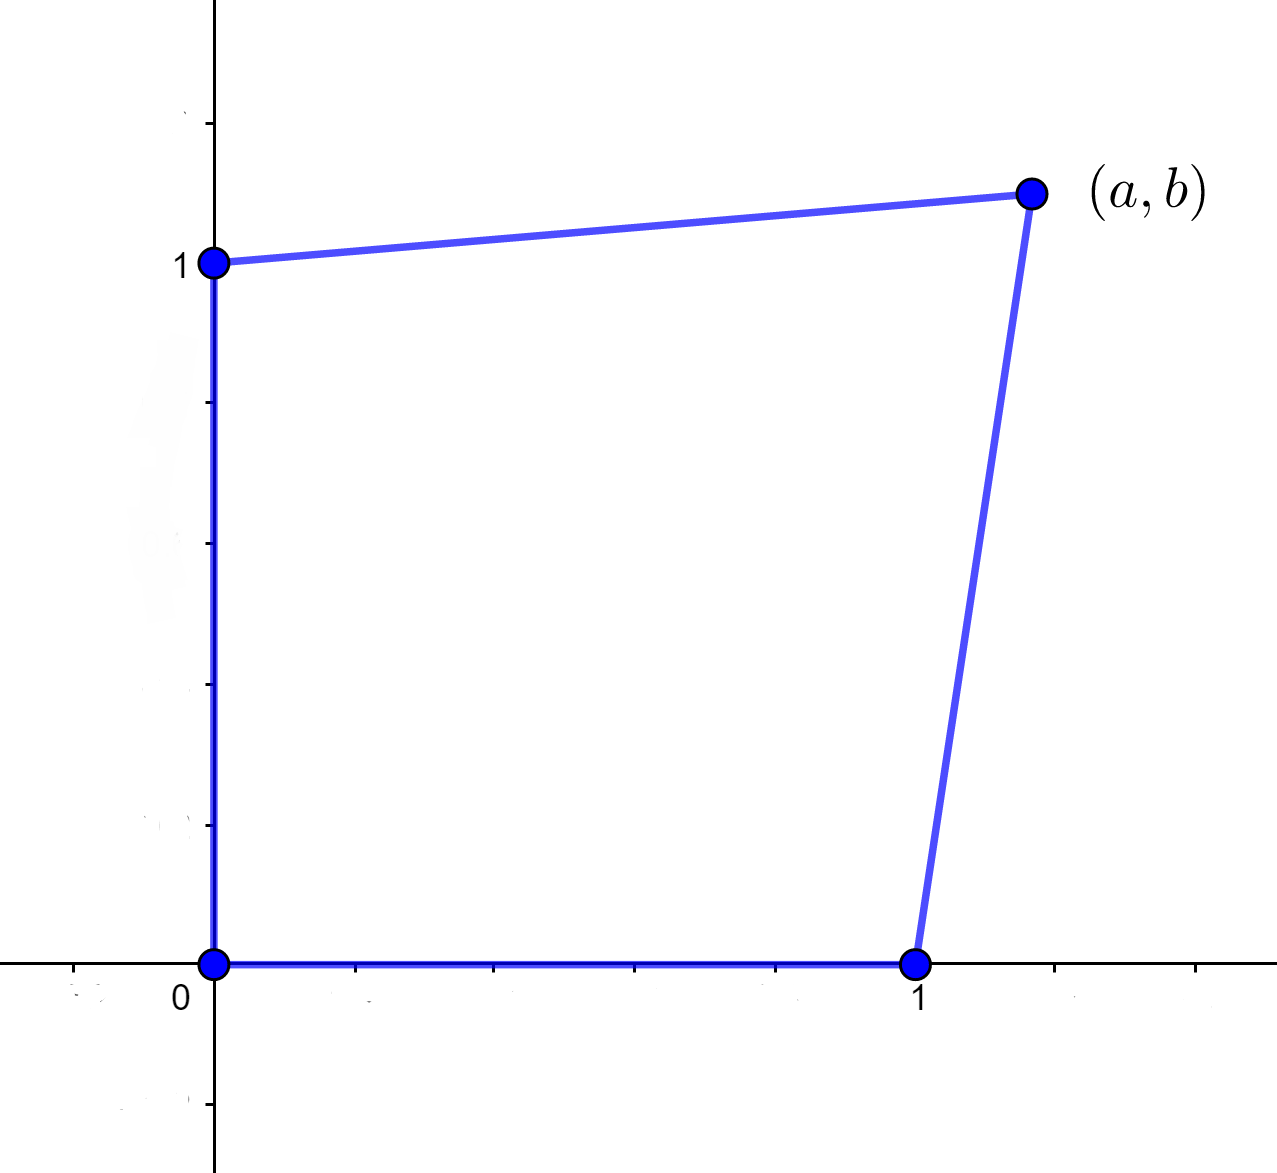
\includegraphics[width=0.35\linewidth]{pic22}
\end{figure}
\noindent
Рассмотрим пучок коник через точки $A_1 = (0,0),\ A_2 = (1,0),\ A_3 = (0,1),\ A_4 = (a,b)$, где $a,b > 0,\ a+b > 1$\\
\begin{gather*}
	C_1: x(x-a) = f(x,y)\\
	C_2: y(y-b) = g(x,y)
\end{gather*}
Пусть пятая точка имеет координаты $A_5 = (c,d)$\\
\begin{gather*}
	C_{A_5} f(A_5) g(A) - g(A_5) f(A) = x(x-a) d(d-b) - y(y-b) c(c-a)
\end{gather*}
Будем считать, что это было в карте $Z = 1$
\begin{gather*}
	\begin{pmatrix}
		0 & \ldots & \ldots\\
		\vdots & d(d-b) & 0\\
		\vdots & 0 & -c(c-a)
	\end{pmatrix}\\
	\\
	\text{det}
	\begin{pmatrix}
	d(d-b) & 0\\
	0 & -c(c-a)
	\end{pmatrix}
	=
	-d(d-b)c(c-a) = A
\end{gather*}
$A > 0$, если $d(d-b)c(c-a) < 0$, в этом случае коника -- эллипс
\begin{figure}[h!]
	\center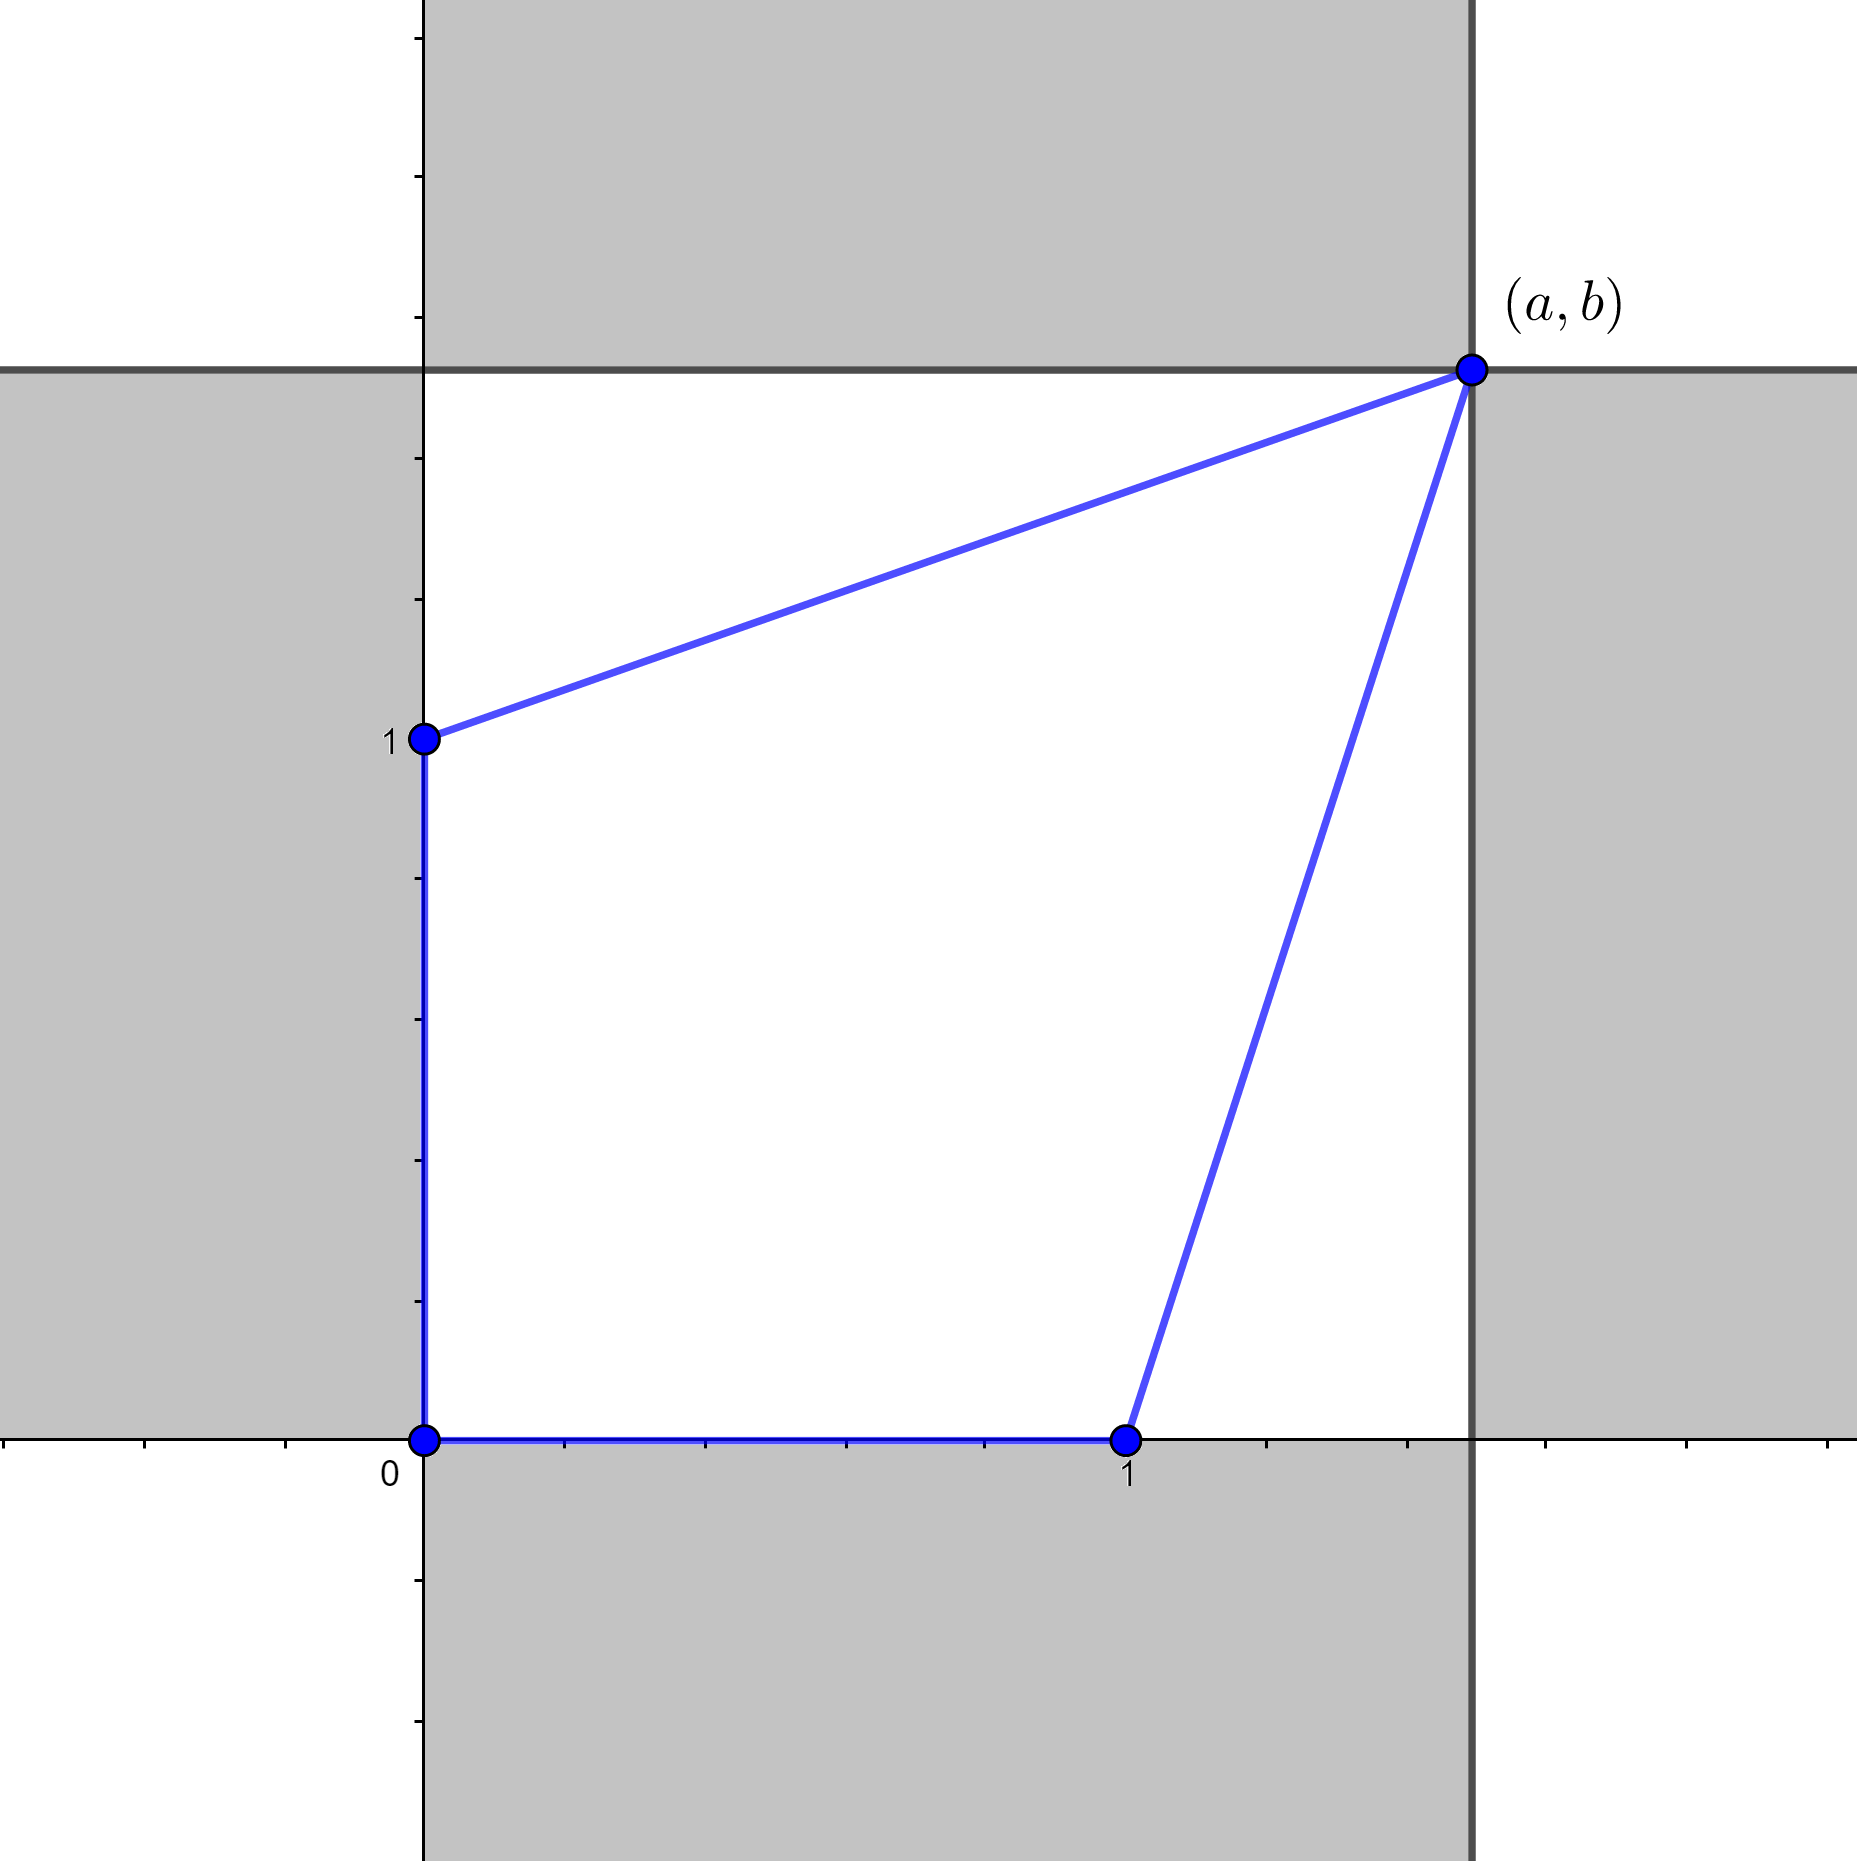
\includegraphics[width=0.35\linewidth]{pic23}
\end{figure} %+
%	\subsection*{ГЛ7 5*}
Рассмотрим октаплекс $\{3,4,3\}$\\
\begin{enumerate}
\item[А] Известно, что $N_0 - N_1 + N_2 - N_3 = 0$\\
	У октаплекса 24 вершины (), ребер $\frac{24 \cdot 8}{2} = 96$ 
	\begin{gather*}
		\begin{matrix}
			\text{размерность} & \text{тип грани и ее количество}\\
			0 & 24\\
			1 & 96\\
			2 & 96\\
			3 & 24\\
			4 & 1
		\end{matrix}
	\end{gather*}
\item[Б] 
\item[В] Правильные октаэдры $\{3,4\}$
\item[Г] Правильные треугольники $\{3\}$

\end{enumerate}
		
	\subsection*{ГЛ10 6}
$\text{sgn}(\text{tr}A^2)$
\begin{enumerate}
\item 
	разберем случай $\text{Mat}_2(\mathbb{R})$\\
	\begin{gather*}
		\text{tr}
		\begin{pmatrix}
			a_{11} & a_{12}\\
			a_{21} & a_{22}
		\end{pmatrix}^2 = a_{11}^2 + 2a_{12}a_{21} + a^2_{22}\\
		q = 
		\begin{pmatrix}
			1 & 0 & 0 & 0\\
			0 & 0 & 2 & 0\\
			0 & 2 & 0 & 0\\
			0 & 0 & 0 & 1						
		\end{pmatrix}
		\quad
		\begin{matrix}
			\Delta_1 > 0\\
			\Delta_2 = 0\\
			\Delta_3 < 0\\
			\Delta_4 < 0
		\end{matrix}
	\end{gather*}
\item 
	$\text{Mat}_{n}(\mathbb{R})$\\
	Всего $n^2$ элементов
	\begin{gather*}
		\text{tr}A^2 = \sum\limits^{n}_{i=1}a^2_{ii} + 2\sum\limits^{n}_{\substack{i<j \\ i = 1}}a_{ij}a_{ji}
	\end{gather*}
	Запишем матрицу грама, упорядочив столбцы по возрастанию суммы индексов:\\
	$a_{11},\ a_{12},\ a_{21},\ a_{22},\ a_{13},\ a_{31},\ a_{23},\ a_{32},\ a_{33},\ldots$\\
	Тогда матрица грама состоит из блоков 
	$\begin{pmatrix}
		0 & 2\\
		2 & 0
	\end{pmatrix} \simeq H^2$
	на диагонали и $1$ при $a_{ii}$\\
	Так как между $a_{k^2k^2}$ и $a_{(k+1)^2(k+1)^2}$ ровно $k$ гиперболических пространств, то $(p_{(k+1)^2-1}, m_{(k+1)^2-1}) = (p_{k^2}+k, m_{k^2}+k)$\\
	Так как знак $\Delta_{(k+1)^2}$ определяется суммой всех $H^2\ ((-1)^{\sum H^2})$, и $\Delta_{(k+1)^2} \cdot \Delta_{(k+1)^2-1} > 0$, следовательно $\text{sgn} = (p_{k^2}+k+1, m_{k^2}+k)$, откуда по индукции получаем:
	\begin{gather*}
		\Delta_{1} > 0\quad (1,0)\\
		\Delta_{2} = 0\\
		\Delta_{3} < 0\\
		\Delta_{4} < 0\quad (3,1)\\
		\Delta_{5} = 0\\
		\Delta_{6} > 0\\
		\Delta_{7} = 0\\
		\Delta_{8} < 0\\
		\Delta_{9} < 0\quad (6,3)\\
		\Delta_{10} = 0\\
		\Delta_{11} > 0\\
		\Delta_{12} = 0\\
		\Delta_{13} < 0\\
		\Delta_{14} = 0\\
		\Delta_{15} > 0\\
		\Delta_{16} > 0\quad (10,6)\\
	\end{gather*}
	Откуда: $\text{sgn}(1+2+\ldots+n, 1+2+\ldots+(n-1)) = \text{sgn}(\frac{1+n}{2}\cdot n, \frac{n}{2}(n-1))$
\end{enumerate}
		 %+
%	\subsection*{ГЛ14 7*}
Докажем задачу методом индукции.\\
Заметим, что при $n=2$ можно дополнить матрицу $D$ строкой единиц сверху, столбцом единиц слева и $0$ в верхнем левом углу и тогда определитель полученной матрицы будет эквивалентен формуле Герона.
\begin{gather*}
	\begin{vmatrix}
		0 & 1 & 1 & 1\\
		1 & 0 & d_{12}^2 & d_{13}^2\\
		1 & d_{12}^2 & 0 & d_{23}^2\\
		1 & d_{13}^2 & d_{23}^2 & 0
	\end{vmatrix}
	= d_{12}^4 + d_{13}^4 + d_{23}^4 + 2(d_{12}^2 d_{13}^2 + d_{12}^2 d_{23}^2 + d_{13}^2 d_{23}^2) =\\
	\\
	(-1)^{3}(d_{12}+d_{13}+d_{23})(d_{12}+d_{13}-d_{23})(d_{12}-d_{13}+d_{23})(-d_{12}+d_{13}+d_{23})\\
\end{gather*}
Откуда следует что он неотрицателен в случае когда треугольник с данными сторонами существует (в случае вырожденного треугольника определитель равен 0).\\
Тогда предположим что утверждение о существовании симплекса доказано для $n = 1, \ldots, k$, докажем тогда что утверждение выполнено и для $n = k+1$\\
Рассмотрим матрицу $D$ размера $(k+1) \times (k+1)$, тогда, по предположению индукции, мы знаем, что существуют $k$ мерные симплексы с вершинами $p_0, \ldots, p_{i-1}, p_{i+1}, \ldots, p_{k+1}$, так как для них выполнено утверждение. 
%	\subsection*{ГЛ10 8}
$f: \Omega_{2n} \simeq \Omega_{2n}$\\
Симплек. группа $\text{Sp}(\Omega_{2n})$
\begin{gather*}
	\text{Sp}_{2n}(k) = \{F \in \text{Mat}_{2n}(k)\ |\ F^t IF = I\}\quad I = 
	\begin{pmatrix}
		0 & E\\
		-E & 0
	\end{pmatrix}
\end{gather*}
Изотропные подпространства:\\
Каждое изотропное подпространство $U_1 \subset \Omega_{2n}$\\
$U_1 \subset L_1$ по определению и $\Omega_{2n} = L_1 \oplus L_1^{\prime}$ (по теореме: $\forall\ L_1\ \exists\ L_1^{\prime}\ |\ V = L_1 \oplus L_1^{\prime}$. Так как каждое изотропное содержится в симплексе $W,\ \text{dim}(W) = 2\text{dim}(U)$)
\begin{gather*}
	\forall U_2 \subset \Omega_{2n}\ \exists L_2\ |\ U_2 \subset L_2
\end{gather*}
и
\begin{gather*}
	\Omega_{2n} = L_2 \oplus L_2^{\prime}
\end{gather*}
Следовательнос существует изометрич. изоморфизм $f: \Omega_{2n} \simeq \Omega_{2n}\quad U_1 \to U_2$\\
\\
Симплектические прдпространства:\\
пусть $W_1 \simeq \Omega_{2k},\ W_2 \simeq \Omega_{2k}$ -- изометрич. изоморфизм\\
$W_1^{\perp}, W_2^{\perp} \simeq \Omega_{2(n-k)}$\\
$W_1 \oplus W_1^{\perp} \simeq \Omega_{2k} + \Omega_{2(n-k)} \simeq W_2 \oplus W_2^{\perp}$\\
Композиция изморфизмов = изоморфизм\\
Базис в\\
$U = L_1 \oplus L_1^{\prime}\quad \langle u \rangle, \langle u^{\prime} \rangle$\\
$V = L_2 \oplus L_2^{\prime}\quad \langle v \rangle, \langle v^{\prime} \rangle$
\begin{gather*}
	\begin{pmatrix}
		u_1 & \ldots & u_n & u_1^{\prime} & \ldots & u_n^{\prime}\\
		0 & \ldots & 0 & 1 & 0 & 0\\
		\vdots & \ddots & \vdots & 0 & \ddots & 0\\
		0 & \ldots & 0 & 0 & \ldots & 1\\
		-1 & 0 & 0 & 0 & \ldots & 0\\
		0 & \ddots & 0 & \vdots & \ddots & \vdots \\
		0 & 0 & -1 & 0 & \ldots & 0\\
	\end{pmatrix}\\
	f(u_i) = V_i\\
	f(u_i^{\prime}) = V_i^{\prime}\\
	\Rightarrow\\
	f \in \text{Sp}(V)\\
	f \mid_{L_1} L_1 \simeq L_2 \Rightarrow \text{Sp}(V) \curvearrowright \{L \subset V\} \text{ транзитивно}
\end{gather*}

%	\subsection*{ГЛ9 9}
%	\subsection*{ГЛ9 10}
Минимальная по включению грань -- это пересечение опорных гиперплоскостей. Заметим, что пересечение аффинных подпространств тоже аффинно. 
\vskip 0.2in
\noindent
Теперь покажем, что $\forall \, v \in \sigma \cap(-\sigma), \ v$ также лежит в этом аффинном подпространстве. Действительно, если $v \in \sigma \cap(-\sigma)$, то вся прямая, натянутая на $v$, лежит в $\sigma$. Она параллельна каждому опорному подпространству (так как иначе она бы пересекла его и не содержалась бы в $\sigma$). Следовательно $v$ лежит в аффинном подпространстве.
		
%	\subsection*{ГЛ13 11*}
		
		
		
		

		
\end{document}